%%% -*-LaTeX-*-

\chapter{Adaptive Sampling with Topology}
\label{ch:adaptiveSampling}

In Section~\ref{sec:adaptiveSampling}, we reviewed the major advances in adaptive sampling.
%
In this chapter, we build upon the concepts presented previously and offer a new perspective by which to select candidates in the adaptive sampling process.
%
Namely, we present methods that seek to exploit areas of high topological significance under different settings.
%
First, we explore new candidate scoring functions in the context of global response accuracy~\cite{MaljovecWangKupresanin2013}.
%
Then, we address selecting batches of candidates in both the global and limit surface cases~\cite{MaljovecWangMoeller2014}.
%
We then conclude this chapter by performing adaptive sampling exclusively in the limit surface case on nuclear power plant safety simulation data~\cite{MaljovecWangMandelli2013b}.

\section{Adaptive Sampling With Topological Scores}
\label{paper:ijuq2013}
In this first work, we look at the problem of desiging experiments in order to globally fit a surrogate model to data that is assumed to be represented by a smooth function.
%
The specific emphasis here is on adaptively sampling the input space based on the response of the surrogate model used.
%
To this end, we explored various combinations of surrogate models, candidate selection criteria, and test functions of varying dimensionality.

\subsection{Methodology}

Two main families of prediction models can be used in uncertainty quantification (UQ): regression models such as MARS and stochastic models such as Gaussian processes.
%
Our general pipeline as illustrated in Figure~\ref{fig:asCycle} is applicable to both families.

We begin by selecting some initial training data, running the simulation and obtaining a collection of true responses at these data points.
%
Second, we fit a prediction model, e.g., a Gaussian process model (GPM), from the initial set of training data.
%
Third, a large set of candidate points is chosen in the parameter space using Latin hypercube sampling (LHS), and the prediciton model is evaluated at these points.
%
The prediction model is used to approximate values at these candidate points and is considered to be a much less expensive surrogate of the ground-truth phenomenon under study.
%
Therefore, we can evaluate a large pool of candidate points relatively quickly and cheaply.
%
Fourth, each candidate point is assigned a score denoting our need to sample it.
%
Finally, the candidate with the highest score is selected and added to the set of training data.
%
This new training data point will be evaluated using the ground-truth and the information discovered will be used to update the prediction model, and the cycle may repeat until an appropriate convergence criterion is met.

Traditional scoring functions are based on either point density, where candidate points that are further away from the existing training data receive higher scores, or on prediction confidence, where candidates with higher prediction uncertainty receive higher scores.
%
In the setting where the underlying data is smooth with little to no noise, the density-based and uncertainty-based strategies will both similarly favor low-density regions because the prediction uncertainty of most prediction models tends to be smallest near the training data.
%
However, such ground-truth models with smooth, uniform behavior are better tackled with space-filling sampling designs that seek to more uniformly cover the input space.
%
Adaptive sampling is better suited for understanding phenomena where the frequency of \emph{toplogical features} is variable, and thus we can focus more samples on higher frequency areas, and reduce sampling where the function is flat or gradually changing.
%
Under these settings, the uncertainty of the predicting model can be quite high near training points if nearby training points are of dramatically different values.
%
For this reason, we propose a third class of scoring functions that more directly targets this topological
information, where candidate points in the area of larger topological changes are assigned higher scores.

\subsubsection{Traditional Scoring Functions}
\label{sec:classic}

We first review several traditional scoring functions that are used as a baseline comparison for our own topological scoring functions.
%
There are three main scoring functions, Delta, ALM and EI, as detailed below.
%
Each funciton is further augmented with a distance penalization factor, creating three additional scoring functions.

Let $\Tcal = \{\z\}_{i=1}^{n}$ be the set of $n$ training points in dimension $d$.
%
The true response at a point $\z \in \Tcal$ is denoted as $y(\z)$.
%
Let $\Scal = \{\x\}_{i=1}^{m}$ be the set of $m$ candidate points in dimension $d$.
%
The predicted response at a point $\x \in \Scal$ is denoted as $\hat{y}(\x)$.

\subsubsubsection{Delta} This criterion can be seen as a way to evenly sample the range space of the function.
%
It is defined as the absolute value of the difference between the predicted response at a candidate point and the response at the nearest training point.
%
Points are chosen wherever the response model predicts a large gap in function value.
%
Although the delta criterion is intuitive, it considers neither gradient magnitudes nor ``predictability.''
%
For example, a point in the middle of a steep but linear ramp is easily predicted even though it may have a large difference in function value.
%
Similarly, a point with a large difference in function value far away from the nearest sample may not be as interesting as a slightly smaller difference in a highly sampled region.
%
Formally, for a point $\x \in \Scal$, $Delta(\x)$ is the absolute difference, to the $q$-th power, between the predicted response and the response observed at the closest point in the training sample, as measured by the $L_p$ distance metric, that is, $d(\x,\x') = (\sum_{i=1}^{d}|x_i-x'_i|^p)^{1/p}$.
%
Said another way, for some fixed parameters $p$ and $q$, let $\x^* = \argmin_{\z \in \Tcal} d(\x,\z)$, then $Delta(\x) = |\hat{y}(\x) - y(\x^*)|^q$.
%
In the default setting, $p = 2$ and $q = 2$.

\subsubsubsection{Active Learning MacKay (ALM)} The ALM criterion, described in~\cite{MacKay1992}, attempts to optimize the predictive variance.
%
The idea is that the variance represents a notion of uncertainty in the prediction, and new samples should be evaluated in the least well understand regions of the parameter space.
%
For the GPM, the variance can be computed directly from the model, which appears to be a significant advantage (see Section~\ref{sec:exp}).
%
For the other prediction models, we use bootstrapping (as described in Sections~\ref{sec:regression} and~\ref{sec:package}) to estimate the variance.

\subsubsubsection{Expected Improvement (EI)}
%
As discussed in Section~\ref{sec:sampling}, EI can be seen as a combination of the expected prediction error used in the ALM method and the Delta criterion.
%
Points are chosen that either show a large uncertainty in their current prediction or have a large discrepancy with the closest existing sample.
%
Our predication model uses $EI(\x) = (|\hat{y}(\x) - y(\x^*)|^2+ ALM(\x))^{1/2}$.

\subsubsubsection{Distance Penalization (DP)} Each of the above three scoring functions can be augmented with a distance penalization factor, thereby creating three additional scoring functions: \emph{DeltaDP}, \emph{ALMDP} and \emph{EIDP}.
%
For DeltaDP, the Delta criterion with an additional penalty term, we can prevent samples from lying too close to the training set.
%
The scaling attempts to balance the goal of sampling in areas of large function variance with the ability to detect yet unknown features by preferring undersampled areas.
%
For a point $\x \in \Scal$, $DeltaDP(\x) = Delta(\x) * \rho_\x$, where $\rho_\x$ is the distance scaling factor.
%
Recall $d_\x = d(\x,\x^*)$ is the distance from $\x$ to the closest point in the training data, and $D$ is a distance vector of $d_\x$ for all $\x \in \Scal$.
%
$\rho_\x = \rho_\x (d_\x, d_0)$, where $d_0$ is the range and $q_0$ is the quantile (by default, $d_0$ is the $q_0$ quantile of $D$).
%
If $d_\x>d_0$, set $\rho_\x = 1$, otherwise $\rho_\x = 1.5d_\x-0.5d_\x^3$, where the coefficients are taken from a spherical semivariogram.
%
Similarly, we define $ALMDP(\x) = ALM(\x) * \rho_\x$, where we approach a more space-filling point selection; and $EIDP(\x) = EI(\x) * \rho_\x$.
%
By default, we use $q_0 = 0.5$.

\subsubsection{Topological Scoring Functions}
\label{sec:toposcoring}
The scoring functions discussed above pick sample points more or less directly based on the idea of globally improving the prediction accuracy.
%
However, these points are not necessarily the optimal candidates.
%
Imagine, for example, a steep mountain that (by random chance) has already been sampled both close to its peak and somewhere near the base.
%
For points on the slope of the mountain, the prediction will show a large difference in function value, thus making it attractive for most standard techniques.
%
However, evaluating the prediction in more detail would also show that even taking a sizable prediction error into account the global structure of the mountain would not change by adding a point on its slope.
%
More specifically, the single mountain would remain a single mountain for a wide range of potential new values, even considering errors and uncertainty.
%
This rationale leads to topology based scoring functions aimed at discovering the global structure -- the topology -- of a function rather than its detailed geometry.
%
In particular, we propose three topology-based scoring functions, \emph{TopoHP}, \emph{TopoP} and \emph{TopoB} as detailed below and illustrated in Figure~\ref{fig:topo-all}.


\subsubsubsection{TopoHP} The first strategy is aimed at sampling at or near predicted critical points with significant influence on the topology.
%
It is defined as the persistence of a candidate point within an (approximated) Morse-Smale complex constructed from oversampling the current response model.
%
Given the current response model, we evaluate its prediction at all candidate points and compute the Morse-Smale complex of the resulting point set by combining both training points and candidate points.
%
We then assign all critical points of the complex that are part of the candidate sets their persistence as score and assign a zero score to all regular points within the candidate sets.
%
Referring to Figure~\ref{fig:topo-all}(a), the silver points illustrate the training points $\Tcal$ and the purple points correspond to the candidate points $\Scal$.
%
We construct a Morse-Smale complex over $\Tcal \cup \Scal$ and return the persistence of the critical points within the candidates.
%
Here, point $\x$ is selected with the highest persistence, and therefore, the highest $TopoHP(\x)$.

\begin{figure}[!t]
\begin{center}
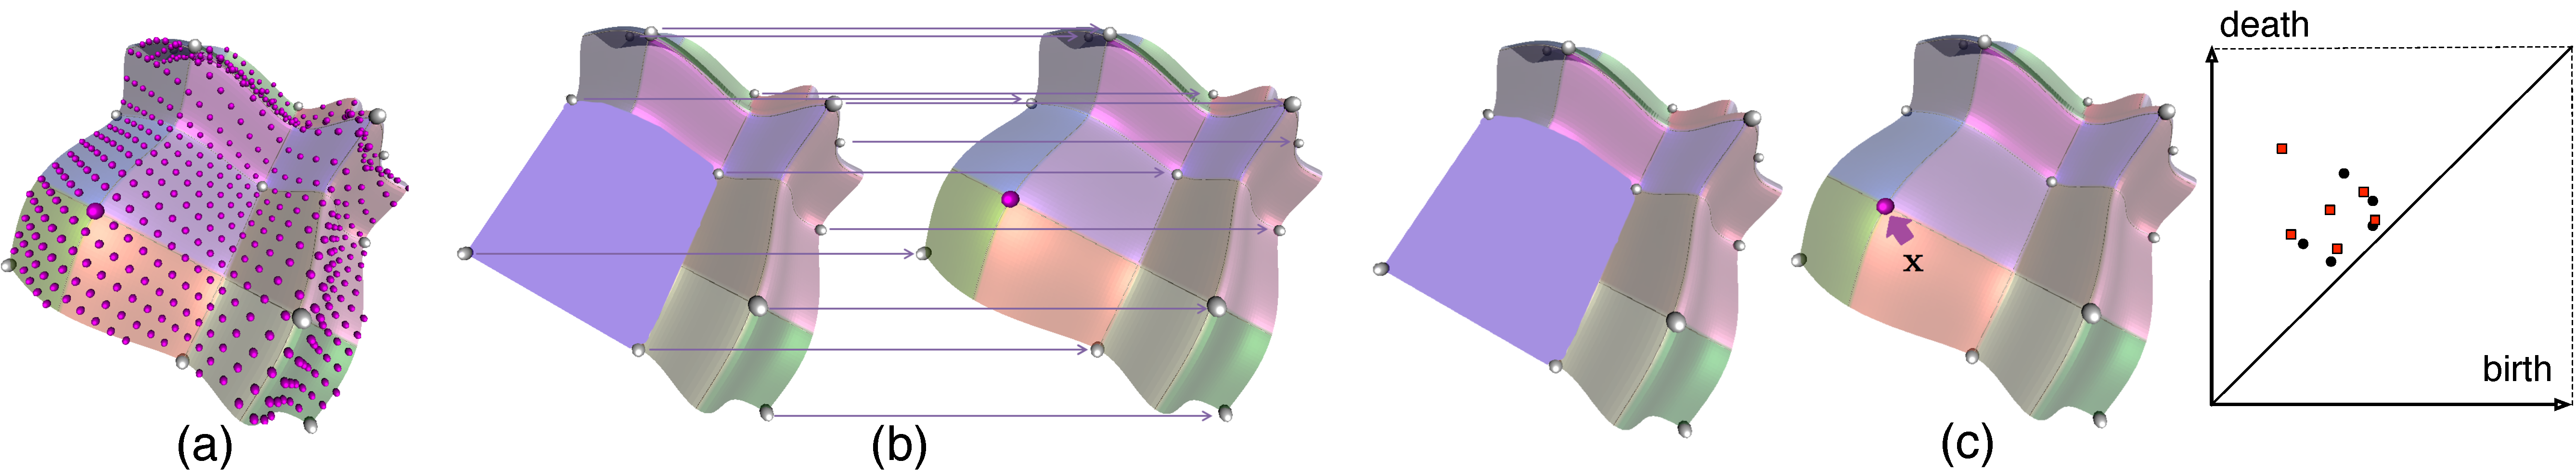
\includegraphics[width=1.0\linewidth]{figs/chap5/topo-all}
\caption{(a) TopoHP: Construct a Morse-Smale complex from training data (silver) as well as all candidates with predicted responses (purple), and return the persistence of the critical points within the candidates.
%
Point $\protect\x$ is selected with the highest $TopoHP(\protect\x)$.
%
(b) TopoP: average change in persistence for all extrema before (left) and after (right) inserting a candidate $\protect\x$ into the Morse-Smale complex.
%
(c) Morse-Smale complexes before (left) and after (middle) inserting a candidate point $\protect\x$;
%
TopoB (right): bottleneck distance between the corresponding persistence diagrams before (circles) and after (squares) insertion.}
\label{fig:topo-all}
\end{center}
\end{figure}

\subsubsubsection{TopoP} Similar to a bootstrapping approach, this strategy aims to evaluate how much the topology (as represented by the persistences) would change if a new candidate point is added.
%
It is defined as the average change of persistence for all current extrema when a given candidate point with its predicted response is inserted into the Morse-Smale complex.
%
As shown in Figure~\ref{fig:topo-all}(b), we first construct the Morse-Smale complex of all training data $\Tcal$ (silver points).
%
Then for each candidate point $\x \in \Scal$, we construct a new Morse-Smale complex consisting of $\Tcal \cup \x$ (Figure~\ref{fig:topo-all}(b) right).
%
To score the candidate $\x$, we compute the change in persistence for each training point $\x \in \Tcal$ that remains as an extrema point between the original and enhanced Morse-Smale complex, and average these changes to obtain a single, non-negative value.

\subsubsubsection{TopoB} For each point $\x \in \Scal$, $TopoB(\x)$ is defined as the bottleneck distance between the persistence diagram of the Morse-Smale complex over $\Tcal$ versus the Morse-Smale complex consisting of $\Tcal \cup \x$.
%
This strategy is similar to the TopoP scoring except that the bottleneck distance takes not only the persistence values into account but also the order and nesting of the corresponding simplification.
%
This strategy is shown in Figure~\ref{fig:topo-all}(c), where left and middle images illustrate the (approximated) Morse-Smale complexes before and after inserting a candidate point $\x$, and the right image displays the corresponding persistence diagrams of these complexes.
%
$TopoB(\x)$ is defined as the bottleneck distance between them.

\subsection{Experiments}
\label{sec:exp}

This section summarizes the different experiments and highlights apparent trends and interesting behaviors.

\subsubsubsection{Example Datasets} To evaluate the different scoring functions and understand the behavior in different scenarios, we have conducted a series of experiments with well-known analytic functions, which can be generalized to high-dimensions.
%
For example, we use a widely used multimodal test function from the optimization literature, the Ackley function~\cite{Ackley1987}, as well as easily controlled test functions such as a Gaussian mixture and the diagonal function.
%
The diagonal function consists of a sine curve aligned with the main diagonal of the unit (hyper-)cube convolved with a Gaussian kernel in the hyperplane orthogonal to the diagonal (see~\cite{GerberBremerPascucci2010}).
%
The diagonal function is attractive for testing because it is not axis aligned, its topological structure is well understood and can be computed analytically, and its complexity is easily controlled.
%
Section~\ref{sec:test} details the closed forms of each function and illustrates their behavior by using two-dimensional contour plots.

\subsubsubsection{Plot and Specifications}
All graphs show the root mean squared error (RMSE) of a given regression model versus the number of samples used for training.
%
The RMSE is computed using points evaluated on a grid.
%
For the two-dimensional case, the total number of points is 2601 evenly spaced at an interval of 0.02.
%
The three-dimensional case uses a total of 9261 points with a grid spacing of 0.05.
%
The four-dimensional case uses a total of 14641 points with a spacing of 0.1, and the 5D case uses a total of 7776 validation points with a spacing of 0.2.
%
All plots show the median RMSE of 10 trial runs.
%
We use the median value since, as discussed below, several regression techniques seem to fail for particular sets of samples, and the median is more robust against the resulting outliers in the RMSE.
%
For a fixed prediction model, all trials start from the same LHS initial training sample $\Tcal$.
%
$|\Tcal| = 20, 30, 100,$ and $200$ in two, three, four, and five dimensions, respectively.
%
Curves are colored by scoring function with the thicker black line indicating an LHS sample of the given size.
%
During each step of the adaptive sampling, a point is chosen among all $|\Scal| =
200*d$ candidate points selected using LHS with the highest score.
%
We have opted to not show variances or percentiles alongside the medians because the resulting plots become too cluttered.
%
Nevertheless, as discussed below, even without an explicit representation several of the plots suggest drastic differences in the stability of the regression.


\begin{figure}[!ht]
\begin{center}
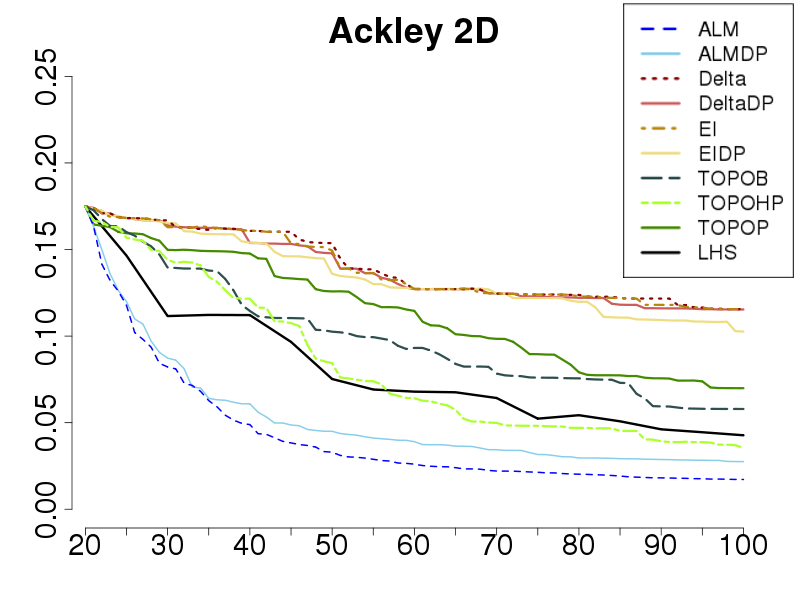
\includegraphics[width=0.45\linewidth]{figs/chap5/gpm_Ackley_td=20}
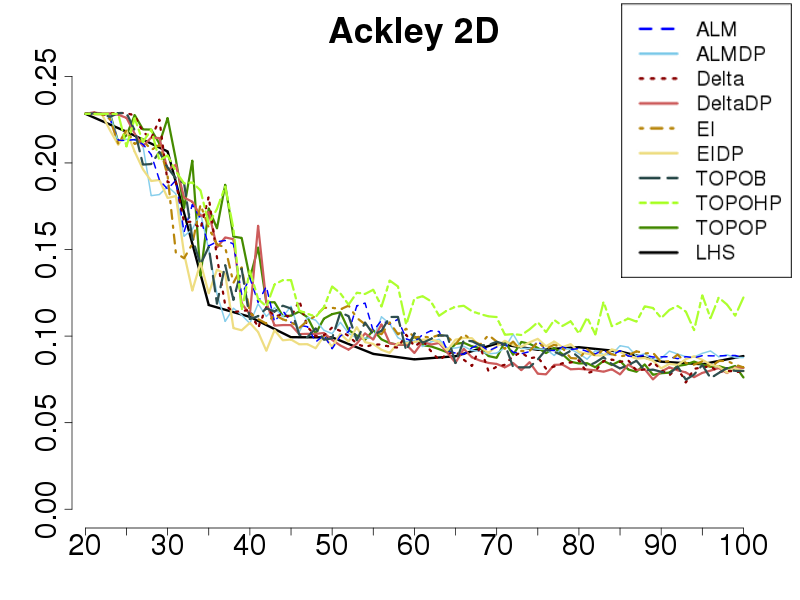
\includegraphics[width=0.45\linewidth]{figs/chap5/earth_Ackley_td=20}
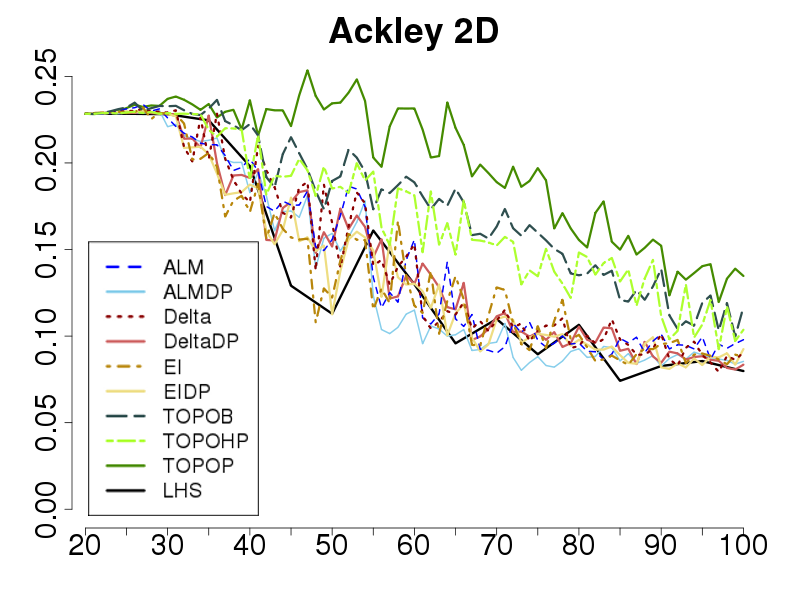
\includegraphics[width=0.45\linewidth]{figs/chap5/mda_Ackley_td=20}
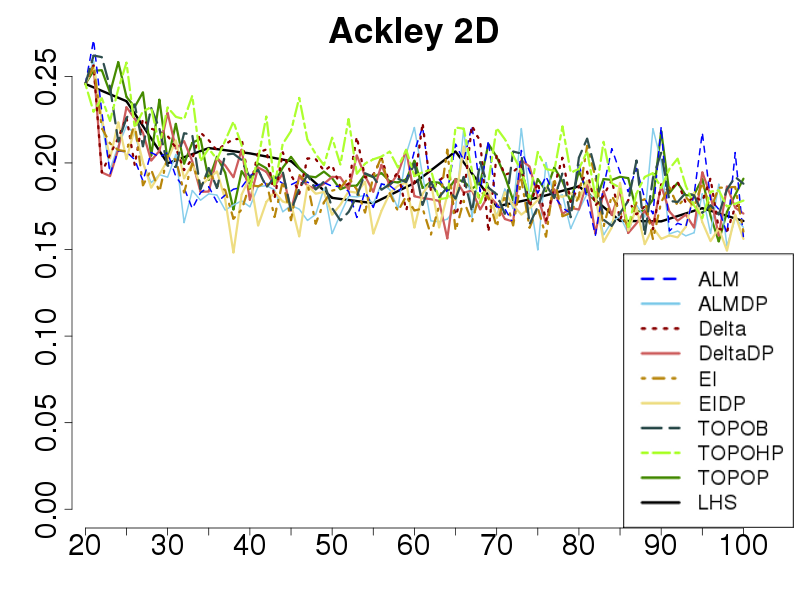
\includegraphics[width=0.45\linewidth]{figs/chap5/nnet_Ackley_td=20}
\caption{Adaptive sampling of the two-dimensional Ackley function using different regression techniques and different scoring functions. From left to right and top to bottom results are shown for the following models: GPM, EARTH, MDA, and NNET.}
\label{fig:ackley2D_results}
\end{center}
\end{figure}

\subsubsubsection{Results} Unsurprisingly, the most significant factor in the success of any scoring function is the quality of the regression model.
%
Unfortunately, many experiments even in lower dimensions failed in the sense that the regression based on the space-filling design did not converge within the number of samples tried.
%
In fact, for some functions some techniques did not show signs of improvement with an increasing number of samples.
%
These results could be improved through manual parameter tuning, but this type of tuning would likely not be feasible in a real-world application where no ground-truth is known and the number of samples is typically severely limited.
%
Furthermore, any manual or semiautomatic parameter tuning would make comparing models even more challenging and potentially bias the results.
%
Therefore, we have selected to run all experiments with the default values provided with the various regression packages listed in Section~\ref{sec:package}.
%
Subsequently, we consider only experiments in which the space-filling design indicated a valid surrogate model.

\begin{figure}[htbp]
\begin{center}
 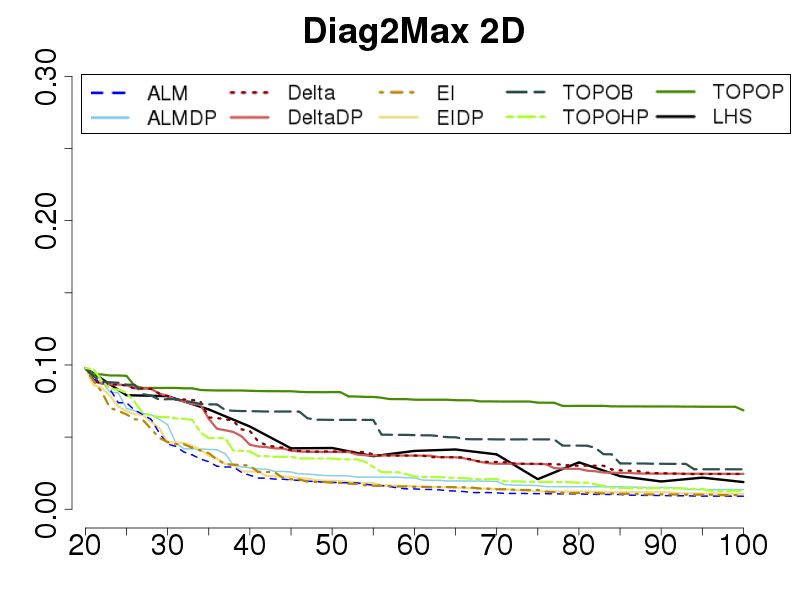
\includegraphics[width=0.45\linewidth]{figs/chap5/gpm_Diag2Max_td=20}
 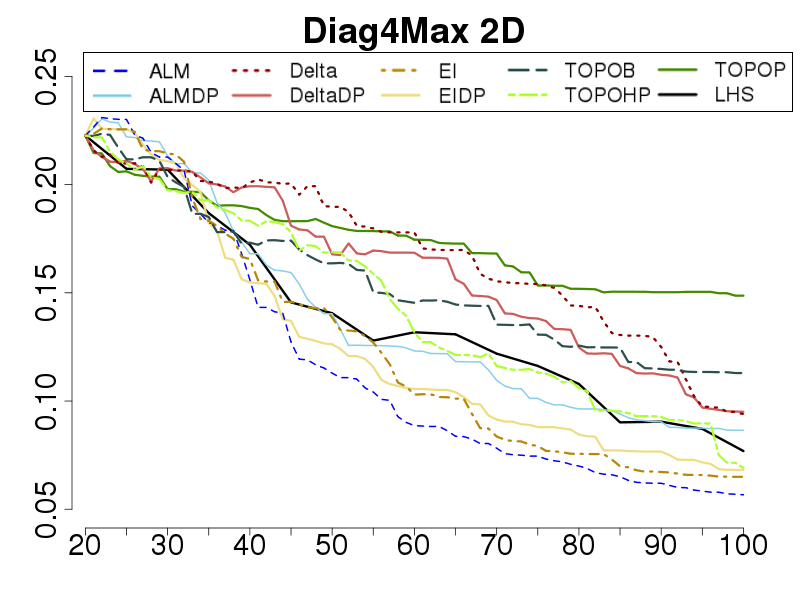
\includegraphics[width=0.45\linewidth]{figs/chap5/gpm_Diag4Max_td=20}
 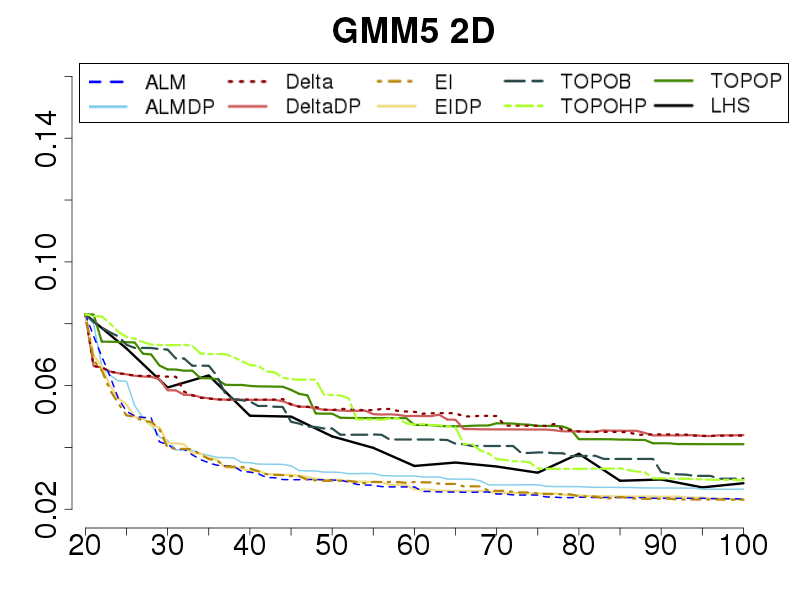
\includegraphics[width=0.45\linewidth]{figs/chap5/gpm_GMM5_2D_td=20}
 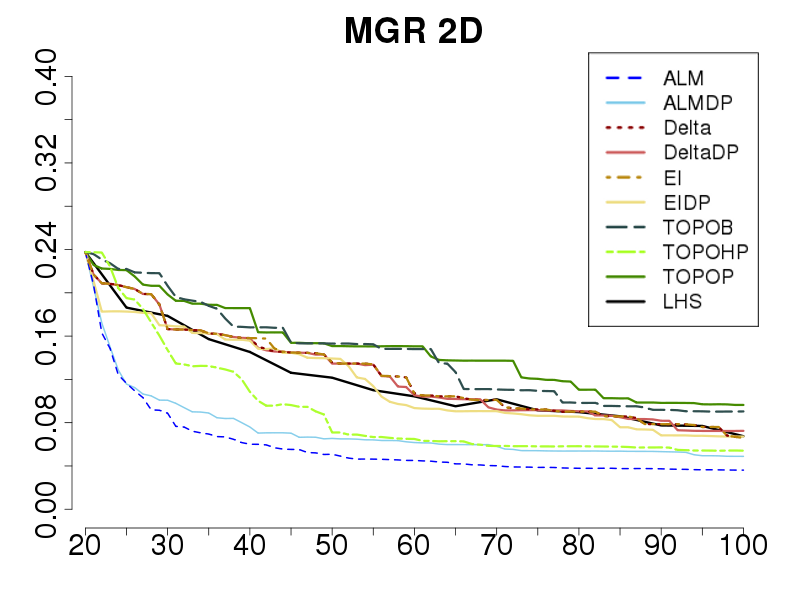
\includegraphics[width=0.45\linewidth]{figs/chap5/gpm_MGR_td=20}
 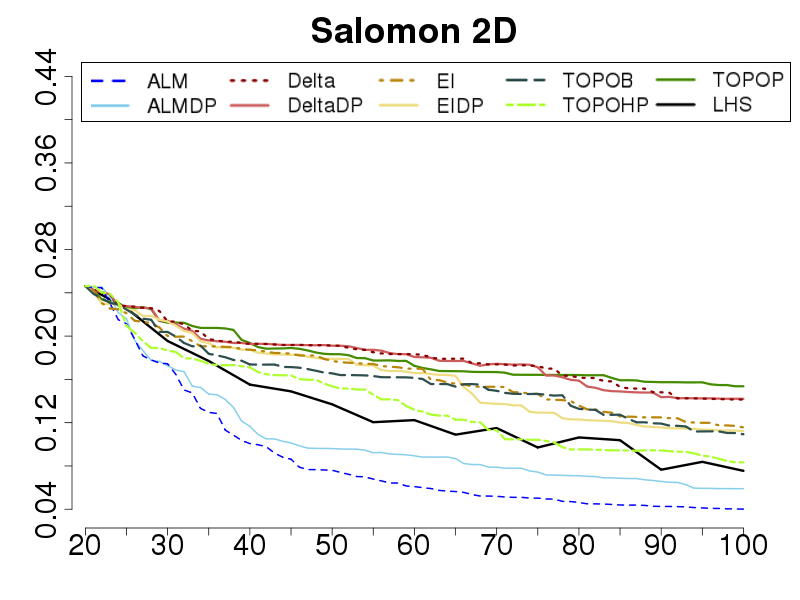
\includegraphics[width=0.45\linewidth]{figs/chap5/gpm_Salomon_td=20}
 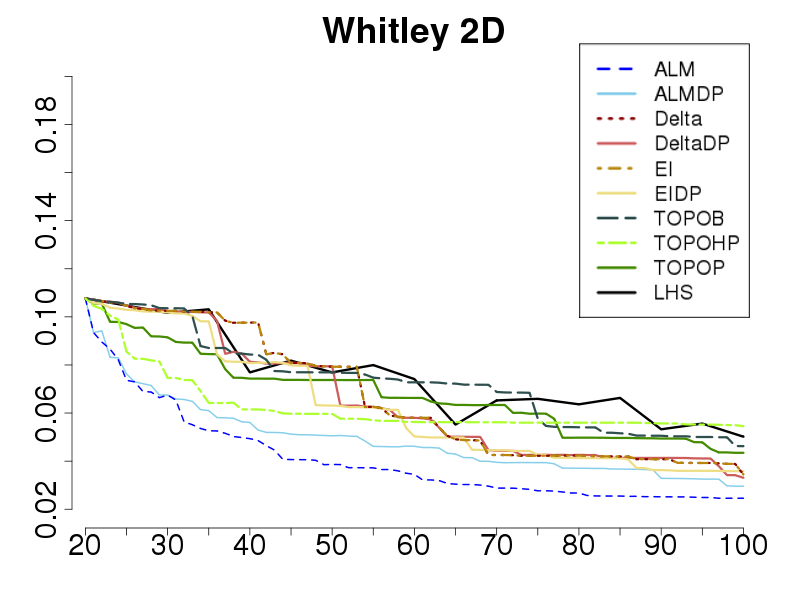
\includegraphics[width=0.45\linewidth]{figs/chap5/gpm_Whitley_td=20}
 \caption{Adaptive sampling various two-dimensional test functions using the GPM. From left to right and top to bottom the following functions are shown: the two-maxima diagonal, the four-maxima diagonal, the mixture of five Gaussians, the MGR, the Salomon, and the Whitley.}
\label{fig:2D_gpm_results}
\end{center}
\end{figure}

In general, the GPM-based regression produces the smoothest and most distinctive plots showing clear differences between scoring functions.
%
Consider the two-dimensional Ackley function shown in Figure~\ref{fig:ackley2D_results}: The ALM criterion significantly outperforms all other scoring functions with the TopoHP being the only other scoring function to beat the space-filling design.
%
Compare the GPM results to the EARTH model shown in the same figure: most scoring functions except TopoHP perform qualitatively similar and barely achieve the same quality as the LHS sampling.
%
Furthermore, all curves are less smooth, suggesting a high variance among the different trials.
%
The other MARS implementation, MDA, performs slightly worse but qualitatively similar with very rough curves without clear trends that fail to achieve the same performance as the space-filling sample.
%
Finally, the NNET implementation barely shows any improvement in RMSE with increasing samples, and all sampling strategies, including the LHS sample, seem to perform similarly with large fluctuations.
%
Overall, NNET achieves by far the worst fit at an RMSE almost an order of magnitude larger than that of the Gaussian process model.

The general differences between regression models seen in the Ackley functions are present for all test functions.
%
Where the GPM models tend to converge for some reasonable number of samples and even in higher dimensions, both MARS implementations have difficulties with non-axis-aligned structures such as the diagonal and the Salomon function.
%
The NNET with the standard parameters consistently performs worse than all other models, and among all techniques only the GPM shows the smoothly converging curves one would traditionally expect.
%
Furthermore, only the GPM model shows significant differences between scoring functions.
%
For the GPM-based adaptive sampling, the one trend observed in most two-dimensional test functions is that the ALM criterion seems to outperform all others.
%
A possible explanation for this behavior is that the predicted variance on which the ALM criterion is based is an integral part of the GPM model itself, which makes the ALM criterion especially well suited for a GPM model and could explain the consistently better performance.

Nevertheless, the performance of the scoring functions even for the well-behaved GPM regression is far from consistent across test functions as seen in Figure~~\ref{fig:2D_gpm_results}.
%
For example, in the diagonal function with two maxima, the ALM and EI criteria perform best, closely followed by TopoHP.
%
The Delta function is on par with the LHS sampling, whereas the other two topological criteria do not perform well.
%
The four-maxima diagonal version shows a similar behavior even though small differences appear between the ALM and EI criteria, and the Delta function now fails to achieve the RMSE of the space-filling sample.
%
The mixture of five Gaussians again shows a clear preference for the error-driven criteria and the Delta function performs worse than the topological scoring functions.

The remaining functions show a very similar pattern with the noticeable exception that now the EI criteria no longer perform as well as the ALM.
%
For the MGR function, TopoHP performs second best, with EI and Delta mirroring the LHS line.
%
For the Salomon function, EI performs better than Delta again, but both fail to beat the space-filling sample.
%
Finally, the Whitley function shows overall a better performance, with EI and Delta both outperforming the topological scoring functions.

The three-dimensional experiments using the GPM show largely similar results, as shown in
Figure~\ref{fig:345D_gpm}.
%
The ALM function generally performs best, with the remaining scoring functions in different combinations behind.
%
However, a notable and interesting exception is the mixtures of two and five Gaussians.
%
For both functions, the Delta criterion performs significantly better than the rest.
%
One explanation is that these functions are characterized by a few large mountains
that, once found, almost entirely determine the function.
%
In such cases, the Delta functional may perform well because it picks values purely based on the observed range.
%
It is unclear, however, why such a behavior is not present in the two-dimensional versions.

\begin{figure}[htbp]
  \begin{center}
   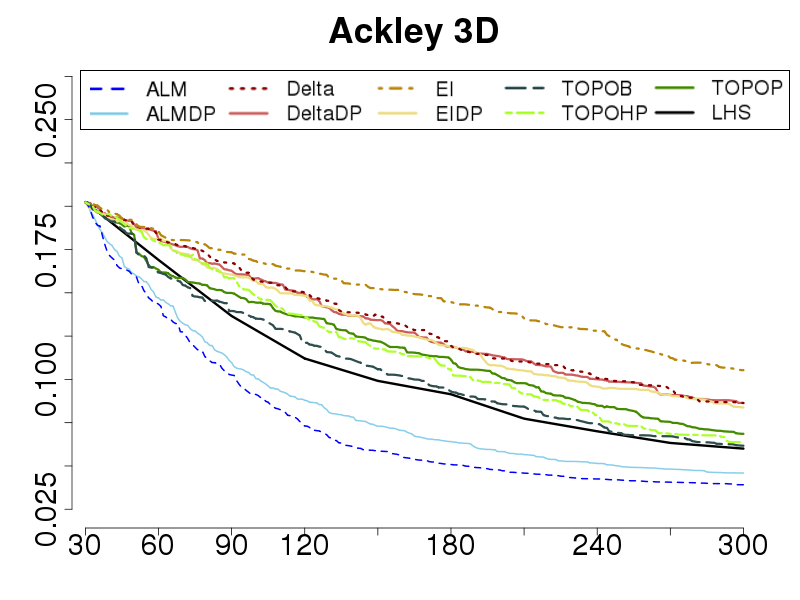
\includegraphics[width=0.24\linewidth]{figs/chap5/gpm_Ackley_td=30}\label{fig:ackley3D_gpm}
   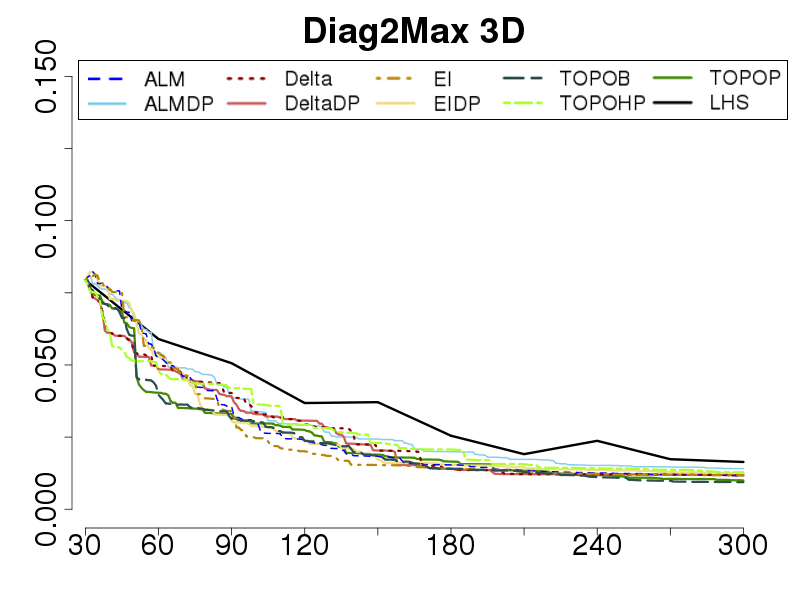
\includegraphics[width=0.24\linewidth]{figs/chap5/gpm_Diag2Max_3D_td=30}\label{fig:2diag3D_gpm}
   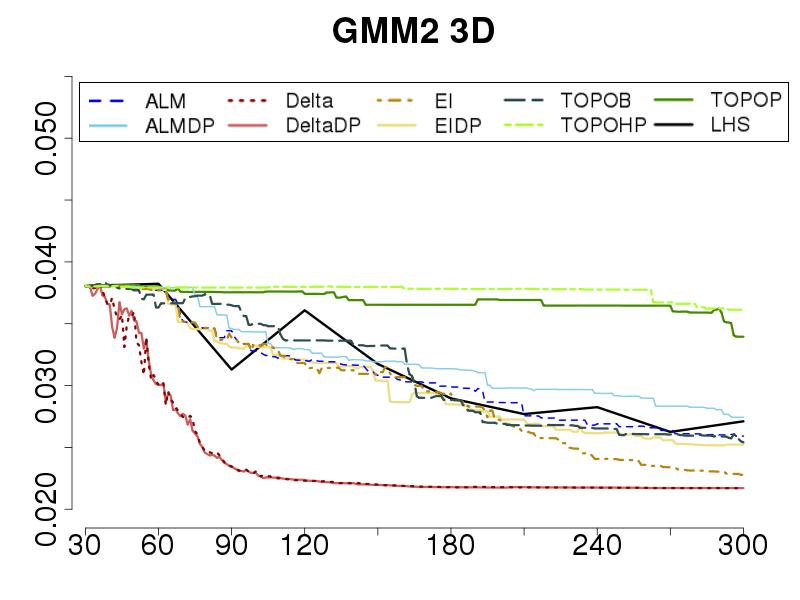
\includegraphics[width=0.24\linewidth]{figs/chap5/gpm_GMM2_3D_td=30}\label{fig:gmm23D_gpm}
   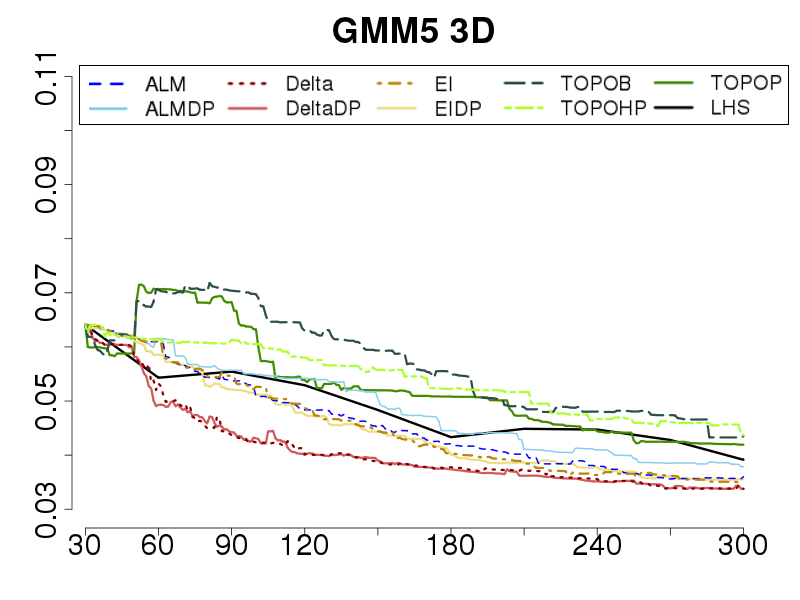
\includegraphics[width=0.24\linewidth]{figs/chap5/gpm_GMM5_3D_td=30}\label{fig:gmm53D_gpm}
   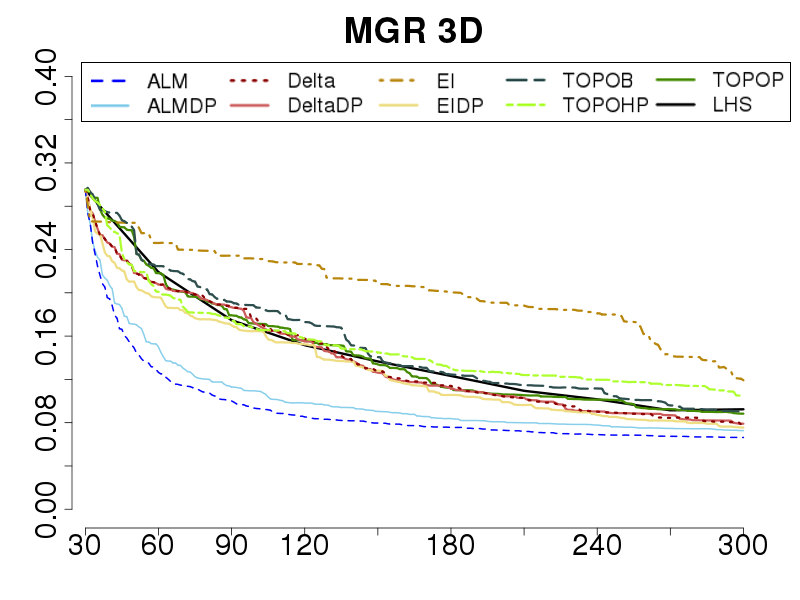
\includegraphics[width=0.24\linewidth]{figs/chap5/gpm_MGR_td=30}\label{fig:mgr3D_gpm}
   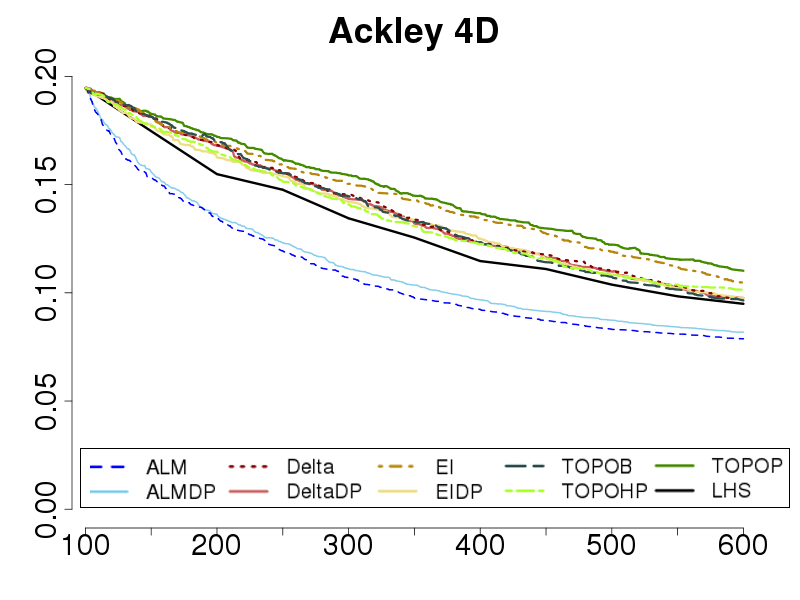
\includegraphics[width=0.24\linewidth]{figs/chap5/gpm_Ackley_td=100}\label{fig:ackley4D_gpm}
   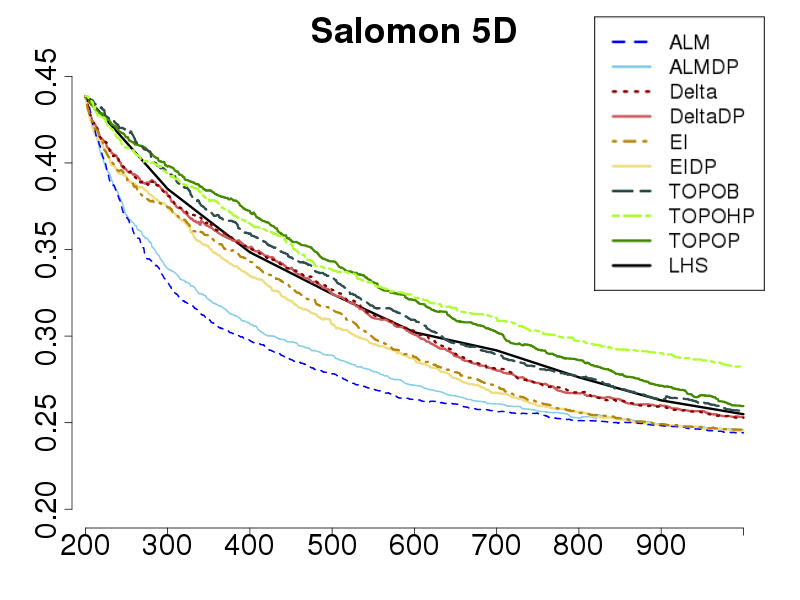
\includegraphics[width=0.24\linewidth]{figs/chap5/gpm_Salomon_td=200}\label{fig:salomon5D_gpm}
   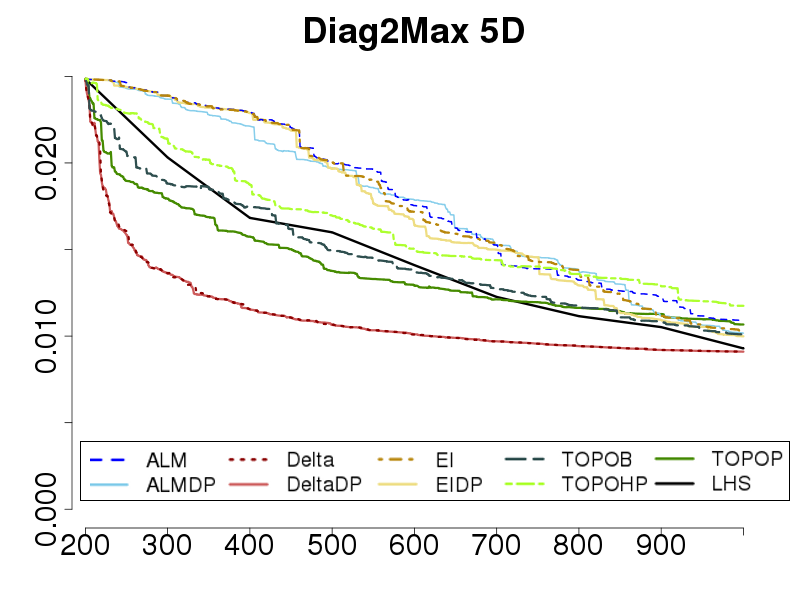
\includegraphics[width=0.24\linewidth]{figs/chap5/gpm_Diag2Max_5D_td=200}\label{fig:2diag5D_gpm}
  \caption{Adaptive sampling of various test functions using the GPM. From left to right and top to bottom the following cases are shown: the three-dimensional Ackley,
  the three-dimensional, two-maxima diagonal, the three-dimensional mixture of two Gaussians, the three-dimensional mixture of five Gaussians, the three-dimensional MGR, the four-dimensional Ackley, the five-dimensional Salomon, and the five-dimensional two-maxima diagonal function.}
  \label{fig:345D_gpm}
  \end{center}
\end{figure}

A similar behavior can be seen in higher dimensions (refer to Figure~\ref{fig:345D_gpm}): The four-dimensional Ackley and the five-dimensional Salomon function show the expected advantage of the ALM criterion, whereas the five-dimensional, two-maxima diagonal function again prefers the Delta criterion.
%
However, in this case all three topological functions outperform the remaining score functions even though they perform on par with only the LHS samples.

As mentioned above, the performance of the other regression techniques is rather spotty, and the results of the adaptive scoring experiments are correspondingly inconsistent.
%
The EARTH model produces results similar to the ones shown in Figure~\ref{fig:ackley2D_results} in case the model itself converges, for example for the two-maxima diagonal function and the mixture of five Gaussians (Figure~\ref{fig:earth_results}).
%
However, considering other experiments listed in the same figure, other experiments show rather large fluctuations in some adaptive sampling curves, e.g., either the TopoHP curve within the MGR function or the LHS curve, e.g., the Whitley function.
%
Overall, the two-dimensional Whitley function shows a good performance, with nearly all adaptive criteria outperforming the LHS curve.
%
Interestingly, in its three-dimensional incarnation, the adaptive sampling does not work nearly as well and also shows excessive variations in several curves.

Still looking at Figure~\ref{fig:earth_results}, in general, there appears to be no significant advantage of one scoring function over another.
However, for many cases with the EARTH model, the TopoHP seems to perform especially bad; for example, see the three-dimensional Whitley and three-dimensional MGR functions.
%
This poor performance is rather surprising since, for the GPM model, TopoHP performed rather well and typically better than the other topological scoring functions.
%
The lack of difference among the other scoring functions is likely due to the error computation.
%
For non-GPM models like MARS, the expected prediction error that forms the basis for both the ALM and the EI criteria is constructed through bootstrapping and thus is probably less reliable.
%
The bootstrapping may negate the differences between error-based criteria and the others, and result in across-the-board worse performance.
%
Unfortunately, we have not been able to get acceptable results for dimensions beyond three, due to the fact that even for simple models like the mixture of two Gaussians, the non-GPM models did not converge.
%
A failed but nevertheless interesting result comes from the mixture of two Gaussians where the model in general shows no real improvements for higher number of points, but both the Delta and the EI criteria first decrease the quality of the fit.

\begin{figure}[t]
\begin{center}
 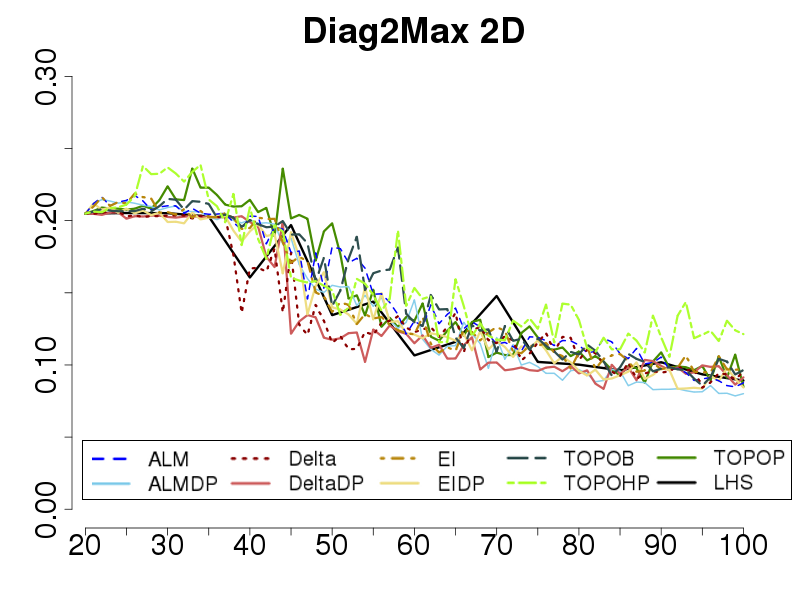
\includegraphics[width=0.45\linewidth]{figs/chap5/earth_Diag2Max_td=20}
 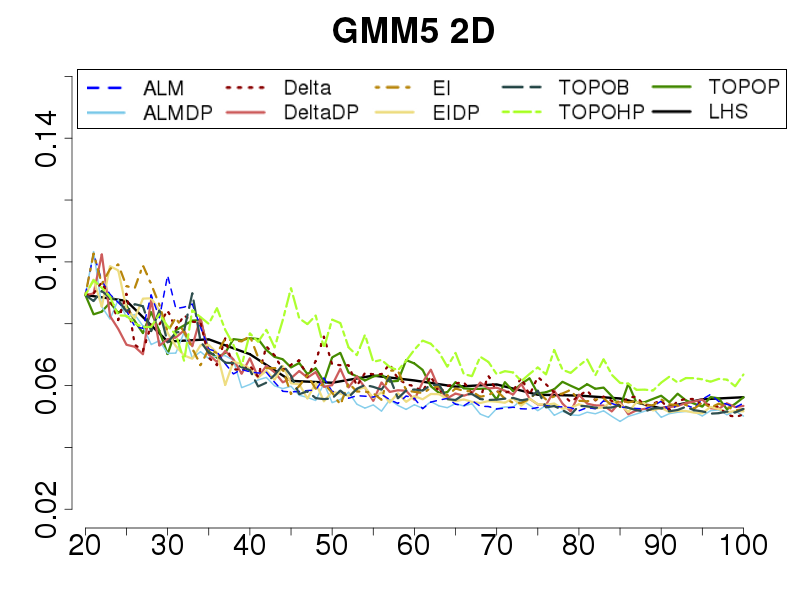
\includegraphics[width=0.45\linewidth]{figs/chap5/earth_GMM5_2D_td=20}
 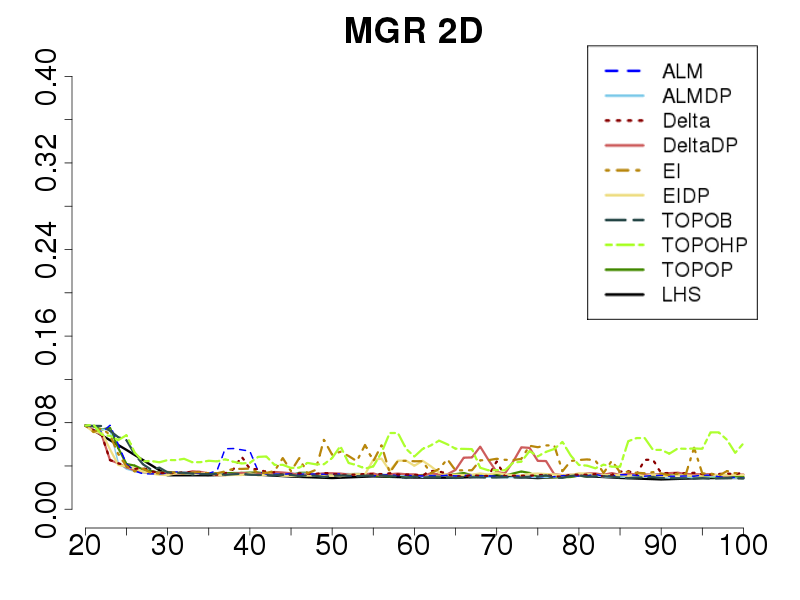
\includegraphics[width=0.45\linewidth]{figs/chap5/earth_MGR_td=20}
 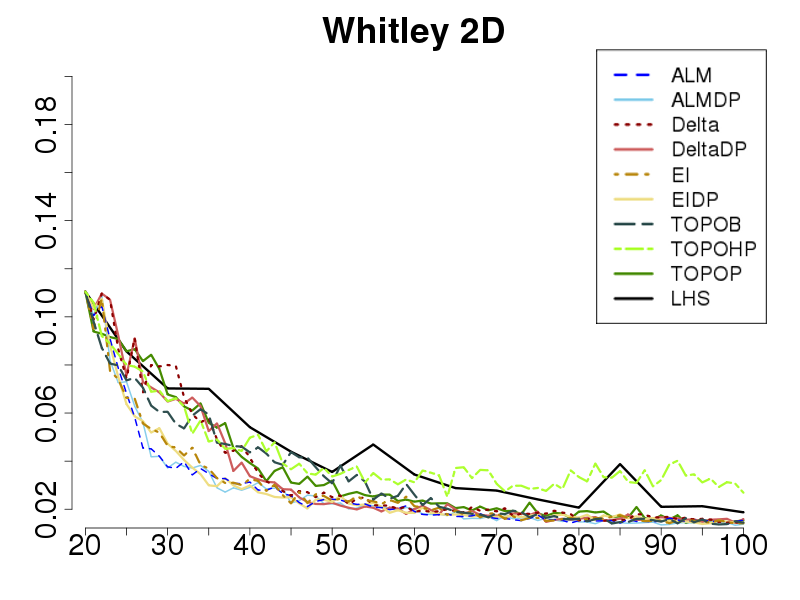
\includegraphics[width=0.45\linewidth]{figs/chap5/earth_Whitley_td=20}
 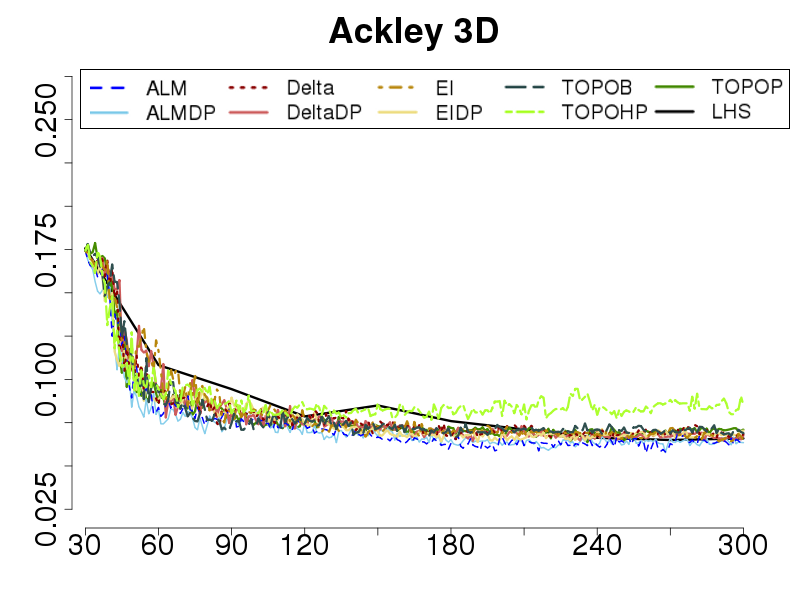
\includegraphics[width=0.45\linewidth]{figs/chap5/earth_Ackley_td=30}
 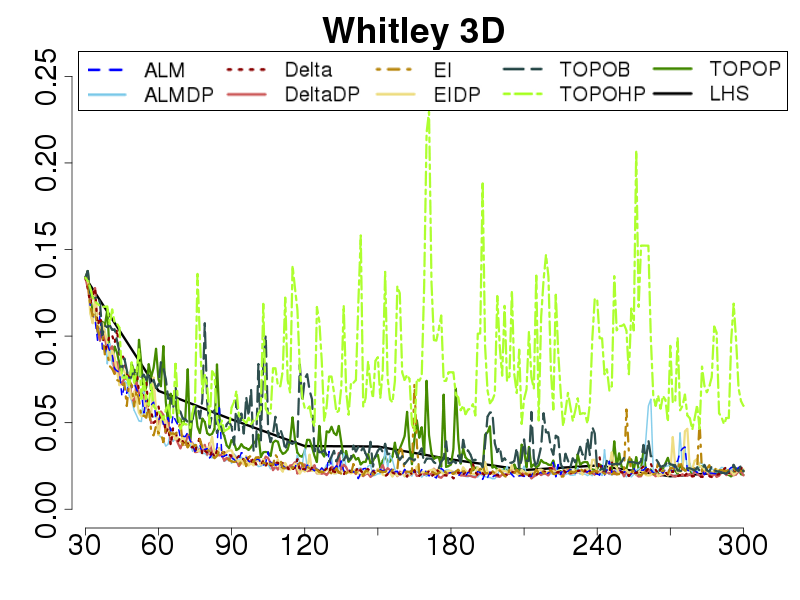
\includegraphics[width=0.45\linewidth]{figs/chap5/earth_Whitley_td=30}
 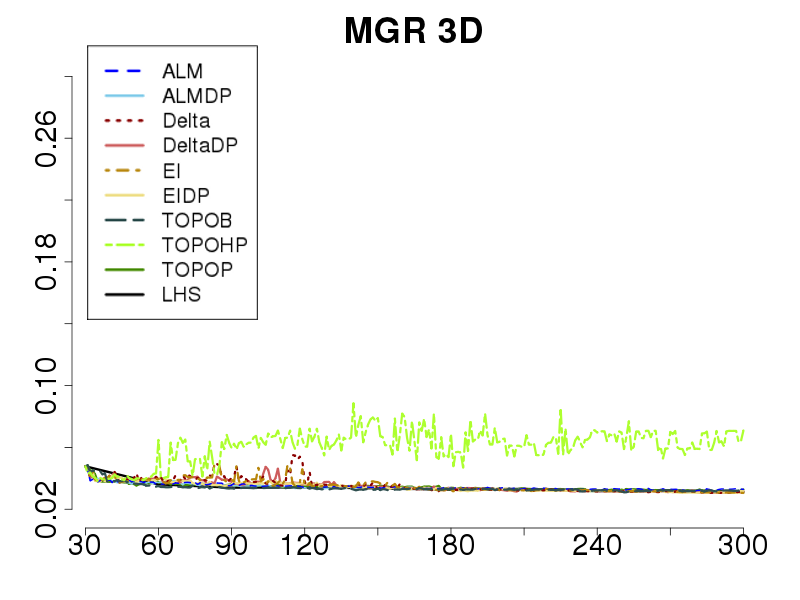
\includegraphics[width=0.45\linewidth]{figs/chap5/earth_MGR_td=30}
 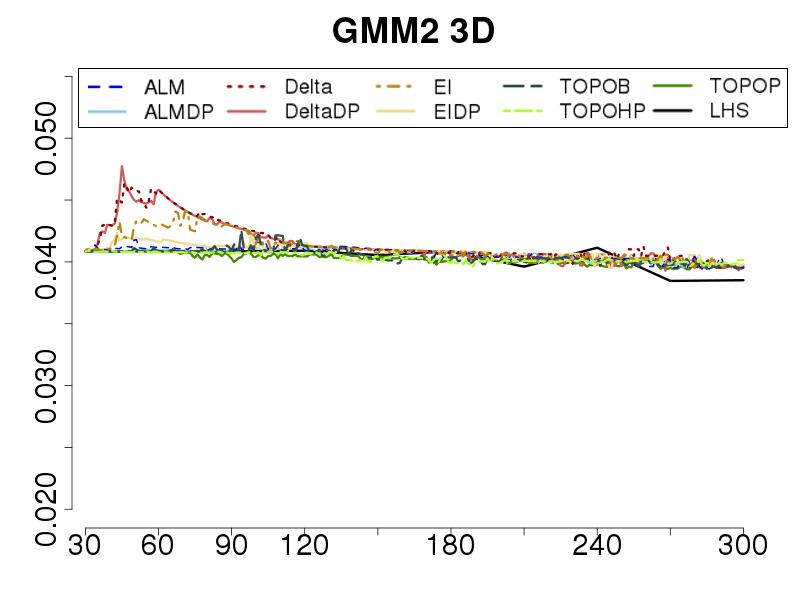
\includegraphics[width=0.45\linewidth]{figs/chap5/earth_GMM2_3D_td=30}
 \caption{Adaptive sampling of various test functions using the EARTH regression model.
 From left to right, top to bottom the graphs for each of the following datasets are shown: the two-dimensional, two-maxima diagonal function, the two-dimensional mixture of five Gaussians, two-dimensional MGR function, the two-dimensional Whitley functions, the three-dimensional Ackley function, the three-dimensional Whitley function, the three-dimensional MGR function, and the three-dimensional mixture of two Gaussians.}
\label{fig:earth_results}
\end{center}
\end{figure}

\begin{figure}[t]
\begin{center}
  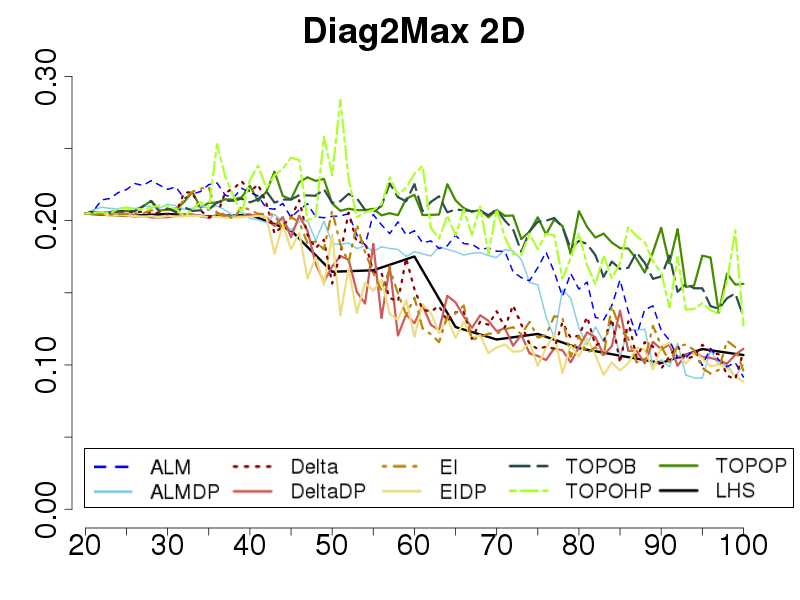
\includegraphics[width=0.45\linewidth]{figs/chap5/mda_Diag2Max_td=20}
  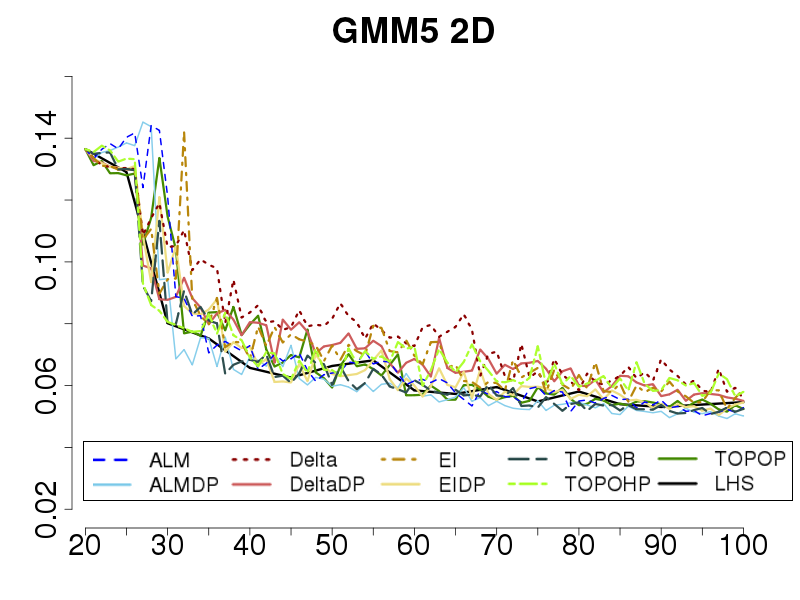
\includegraphics[width=0.45\linewidth]{figs/chap5/mda_GMM5_2D_td=20}
  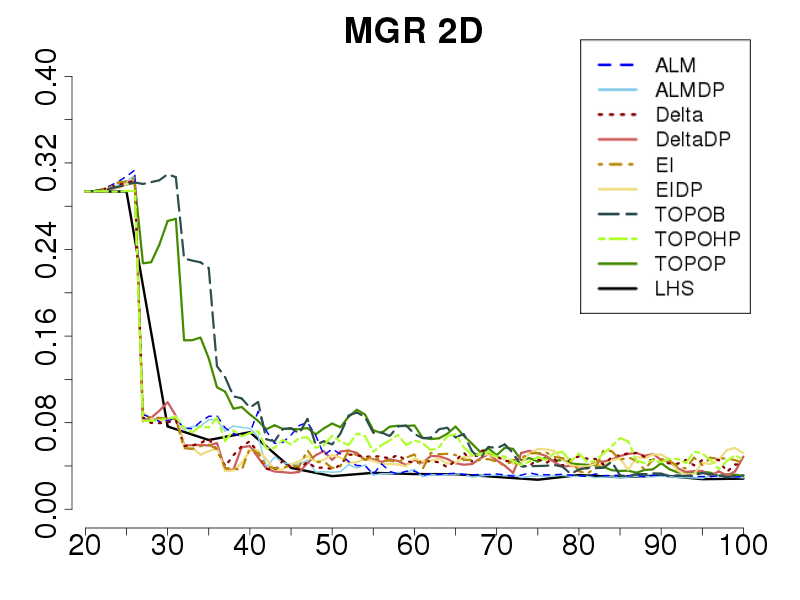
\includegraphics[width=0.45\linewidth]{figs/chap5/mda_MGR_td=20}
  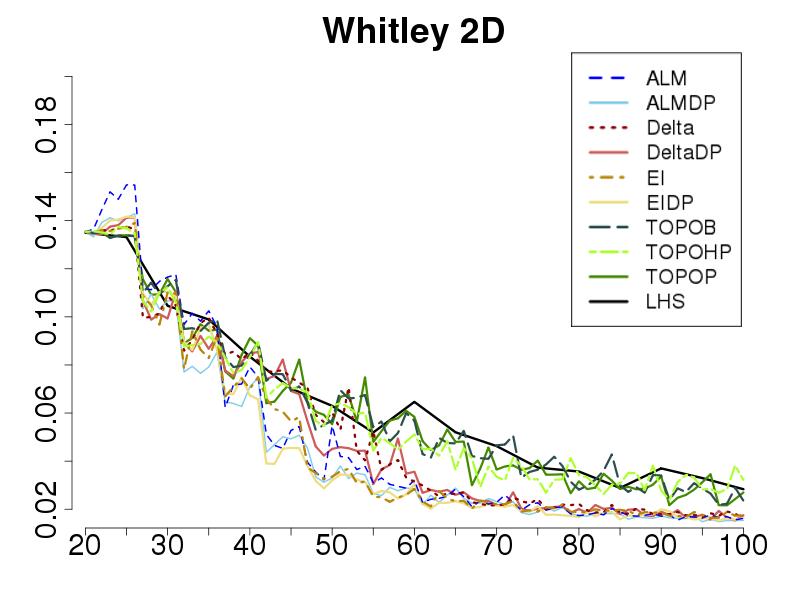
\includegraphics[width=0.45\linewidth]{figs/chap5/mda_Whitley_td=20}
  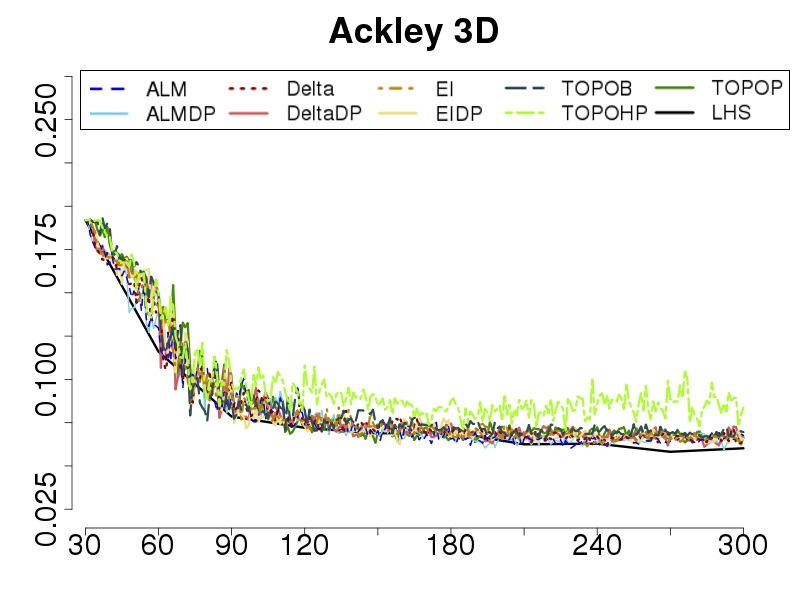
\includegraphics[width=0.45\linewidth]{figs/chap5/mda_Ackley_td=30}
  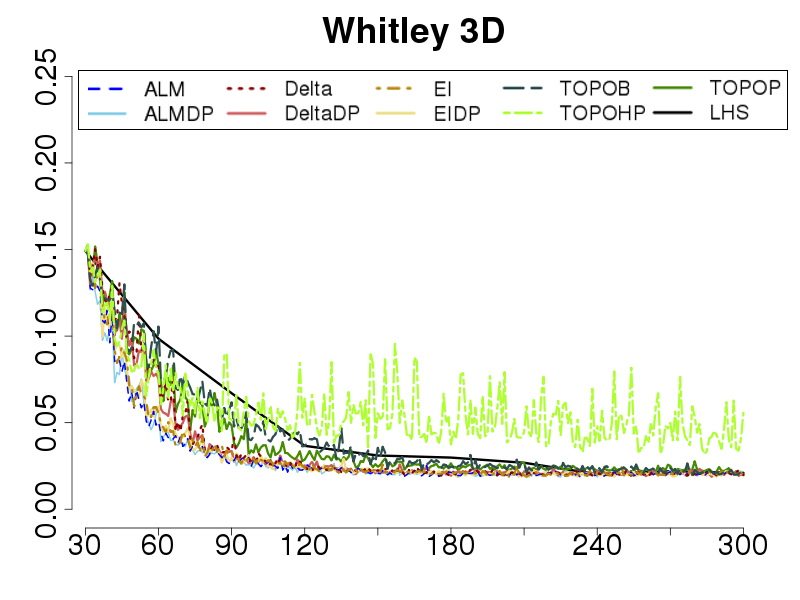
\includegraphics[width=0.45\linewidth]{figs/chap5/mda_Whitley_td=30}
  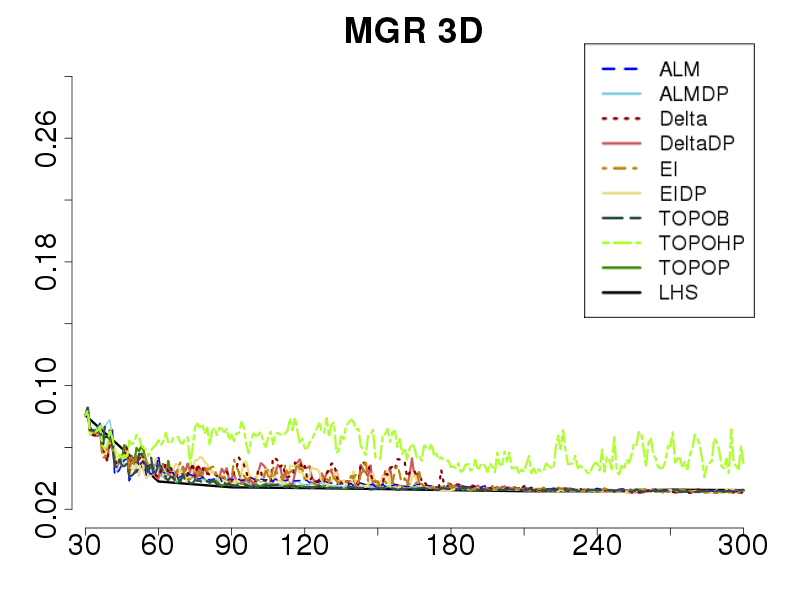
\includegraphics[width=0.45\linewidth]{figs/chap5/mda_MGR_td=30}
  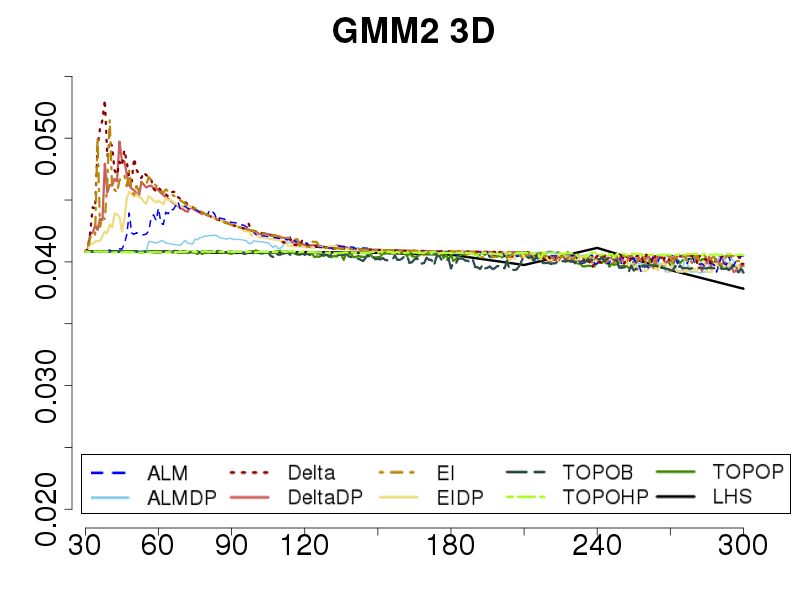
\includegraphics[width=0.45\linewidth]{figs/chap5/mda_GMM2_3D_td=30}
\caption{Adaptive sampling of various test functions using the MDA model. From left to right and top to bottom, the plots for the following cases are shown: the two-dimensional two-maxima diagonal, the two-dimensional mixture of five Gaussians, the two-dimensional MGR function, the two-dimensional Whitley function, the three-dimensional Ackley function, the three-dimensional Whitley function, the three-dimensional MGR function, and the three-dimensional mixture of two Gaussians.}
\label{fig:mda}
\end{center}
\end{figure}

The other MARS implementation MDA, unsurprisingly, shows largely the same behavior as EARTH.
%
Figure~\ref{fig:mda} shows four examples, each in two and three dimensions.
%
Comparing with the Earth model, we see typically comparable RMSE and higher variability (e.g., the two-diagonal and GMM functions in two-dimensional) with the exception of the three-dimensional Whitley function.
%
Again, the three-dimensional mixture of two Gaussians shows the initial decrease in RMSE for several scoring functions.

\begin{figure}[t]
\begin{center}
  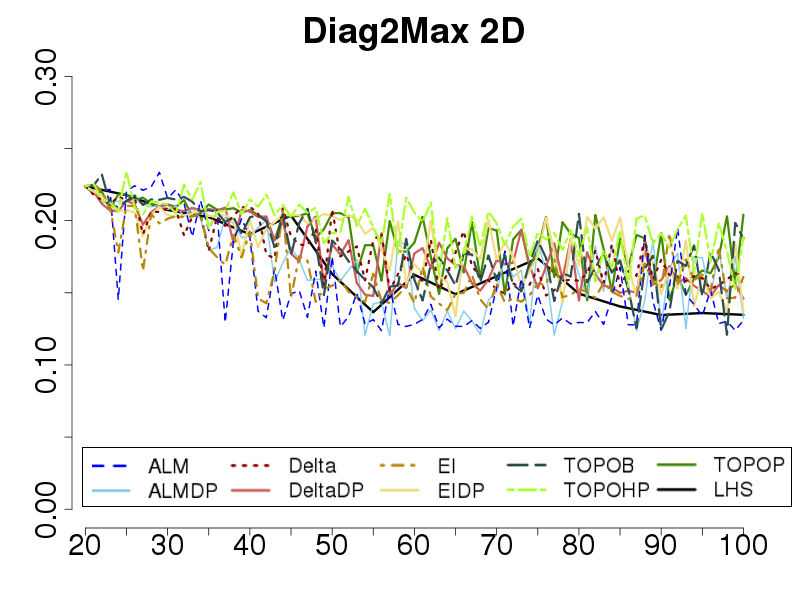
\includegraphics[width=0.48\linewidth]{figs/chap5/nnet_Diag2Max_td=20}\label{fig:2diag2D_nnet}
  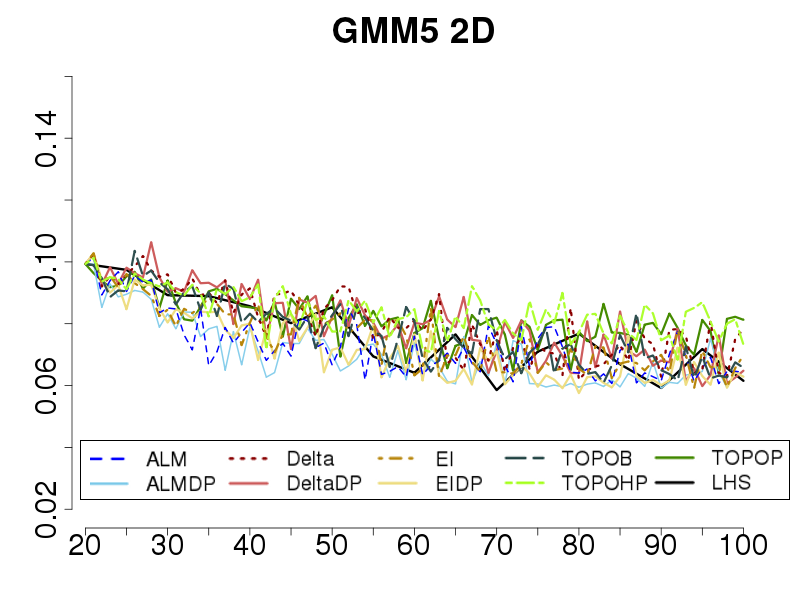
\includegraphics[width=0.48\linewidth]{figs/chap5/nnet_GMM5_2D_td=20}\label{fig:gmm52D_nnet}
  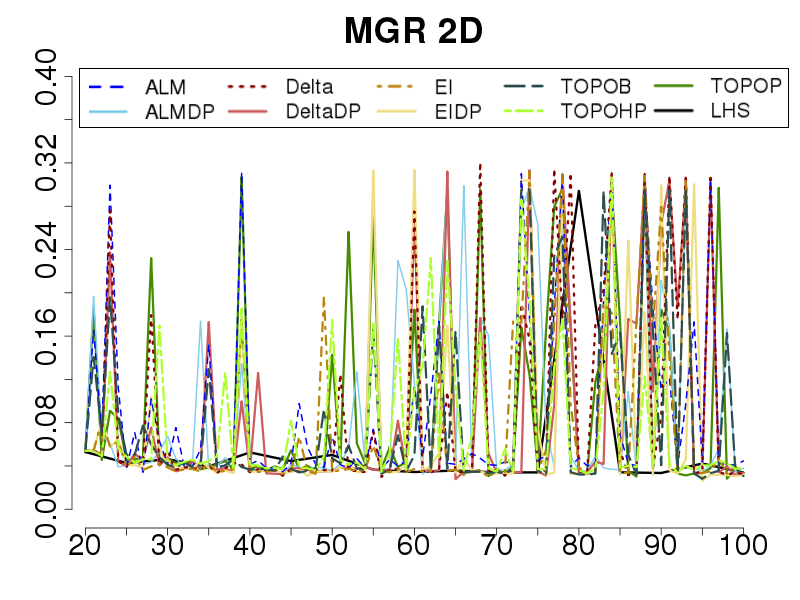
\includegraphics[width=0.48\linewidth]{figs/chap5/nnet_MGR_td=20}\label{fig:mgr2D_nnet}
  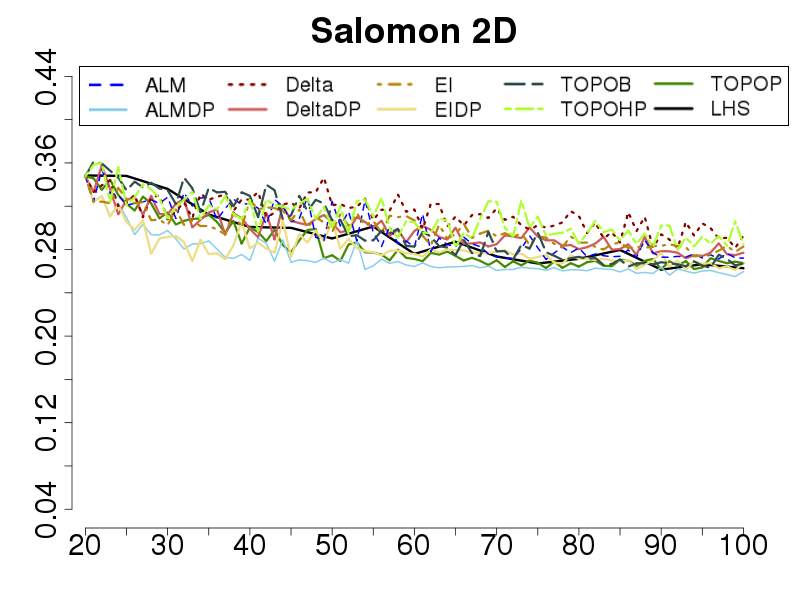
\includegraphics[width=0.48\linewidth]{figs/chap5/nnet_Salomon_td=20}\label{fig:salomon2D_nnet}
\caption{Adaptive sampling of various two-dimensional test functions using the NNET model. From left to right and top to bottom the following cases are shown: the two-maxima diagonal function, the mixture of five Gaussians, the MGR function, and the Salomon function.}
\label{fig:nnet_2D}
\end{center}
\end{figure}

\begin{figure}[t]
\begin{center}
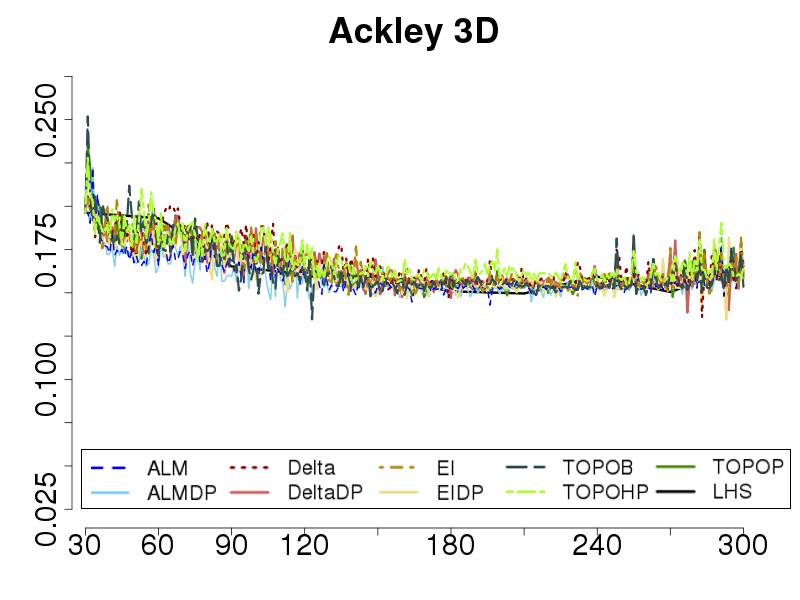
\includegraphics[width=0.48\linewidth]{figs/chap5/nnet_Ackley_td=30}\label{fig:ackley3D_nnet}
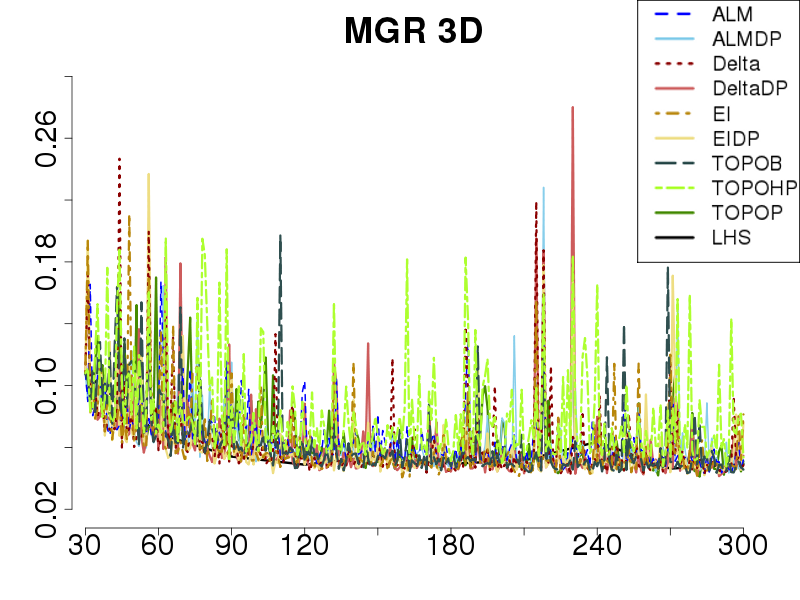
\includegraphics[width=0.48\linewidth]{figs/chap5/nnet_MGR_td=30}\label{fig:mgr3D_nnet}
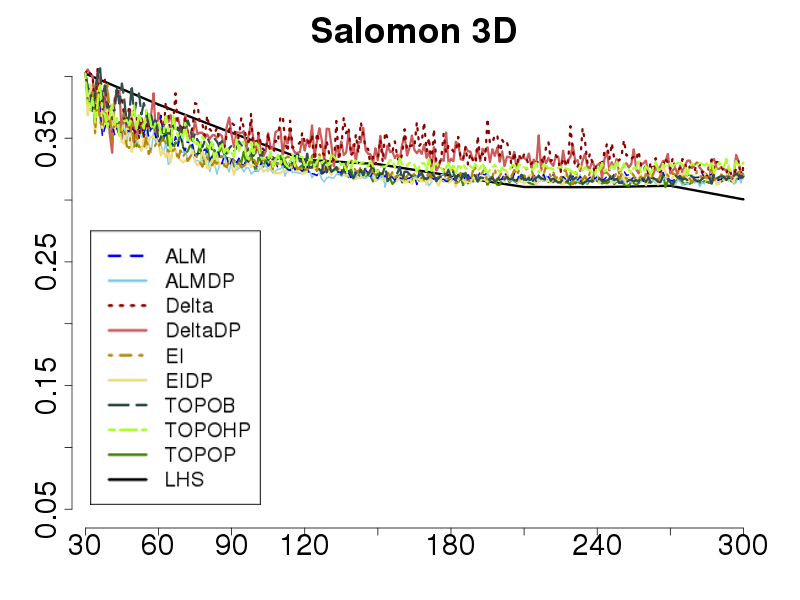
\includegraphics[width=0.48\linewidth]{figs/chap5/nnet_Salomon_td=30}\label{fig:salomon3D_nnet}
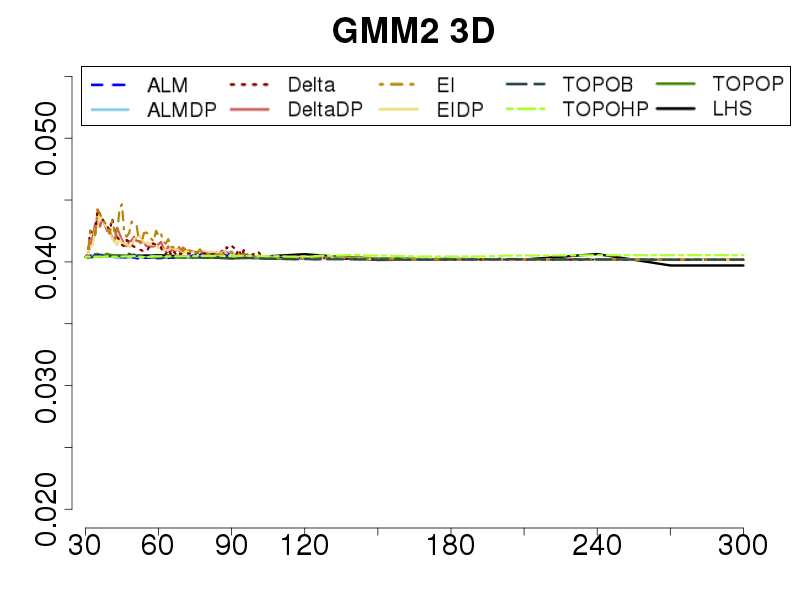
\includegraphics[width=0.48\linewidth]{figs/chap5/nnet_GMM2_3D_td=30}\label{fig:gmm23D_nnet}
\caption{Adaptive sampling of various three-dimensional test functions using the
  NNET model. From left to right and top to bottom the following cases are shown: the Ackley function, the MGR function, the Salomon function, and the mixture of two Gaussians.}
  \label{fig:nnet_3D}
\end{center}
\end{figure}

Finally, the NNET implementation in its default setting, whose results are summarized in Figures~\ref{fig:nnet_2D} and~\ref{fig:nnet_3D}, performs clearly worse, with excessive variability in all plots, which makes interpretation of any possible trends questionable.
%
Apart from the Ackley function, some models that performed reasonably in two dimensions are the two-maxima diagonal function, the mixture of five Gaussians, and the Salomon function.
%
The MGR function shows a competitive RMSE as a baseline but excessive variations for virtually all adaptive scoring functions as well as the LHS line.
%
The three-dimensional MGR function shows a similar behavior except that the LHS line now appears to be stable.

The three-dimensional Ackley and Salomon functions both show the high variability and high RMSE with no adaptive scoring functions able to outperform the space-filling sampling.
%
Just as with the two MARS implementations, the three-dimensional mixture of two Gaussians does not improve with an increasing number of samples and shows the initial increase in RMSE for some scoring functions.

\subsection{Discussion}

After running an extensive set of experiments in two to five dimensions with nine different scoring functions, some general trends appear even though the fundamental question of which particular scoring function to use remains largely inconclusive.
%
The results listed above are only a small first step in this direction.
%
The first not necessarily surprisingly result is that the quality of the underlying regression model plays a key role in the performance of any adaptive sampling technique.
%
In this study, the GPM model performs the best and is the only one showing significant differences between scoring functions.
%
Overall, it seems that the combination of ALM and GPM is the preferred choice, even though some functions perform well with the Delta criteria.

The remaining regression models all show problems fitting many of the test functions, and the large variability suggests that they are sensitive to specific sample locations.
%
In the cases where reasonable fits have been achieved, all scoring functions perform equally well (or poorly).

The new topological scoring functions are largely competitive in terms of RMSE and often perform among the top scoring functions.
%
Some results suggest that detailed fits with a high number of samples are less well suited for topological scoring functions since they are designed to recover larger scale features.
%
Nevertheless, topological scoring functions are expected to better recover the global structure of a function, and finding quantitative metrics to test this hypothesis as well as expanding the class of such functions will be the focus of future research.

\subsection{Example Test Functions Closed Forms and Plots}
\label{sec:test}

\begin{figure}[htbp]
\begin{center}
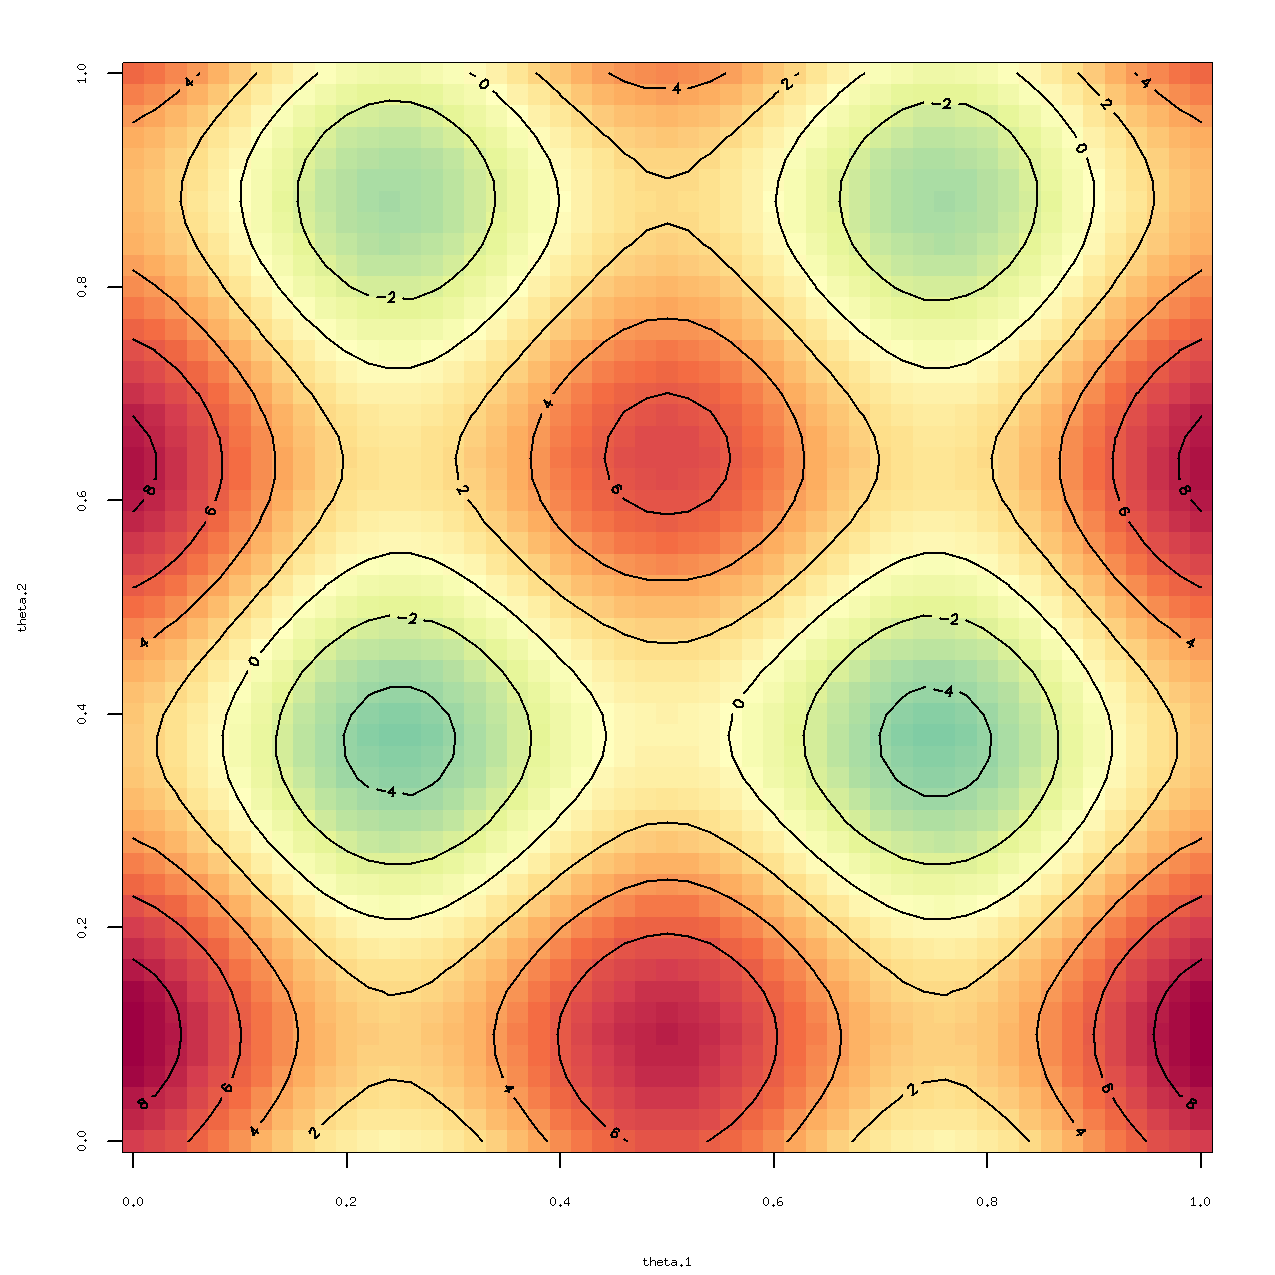
\includegraphics[width=0.24\linewidth]{figs/chap5/Ackley.png}
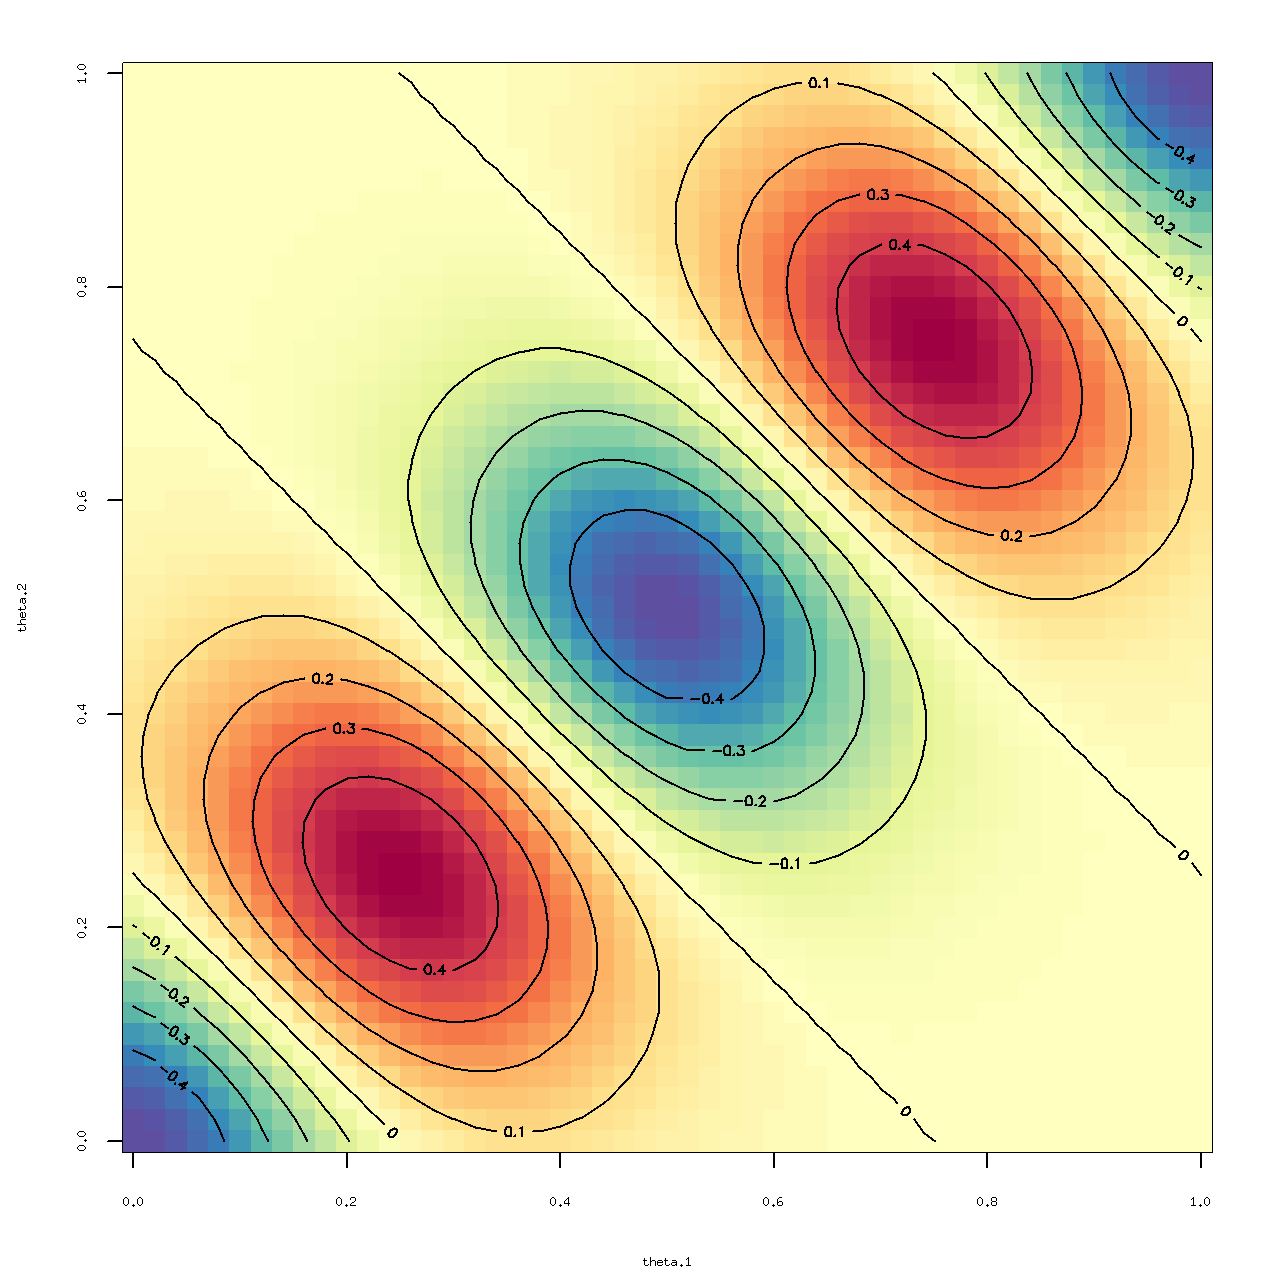
\includegraphics[width=0.24\linewidth]{figs/chap5/Diag2Max.png}
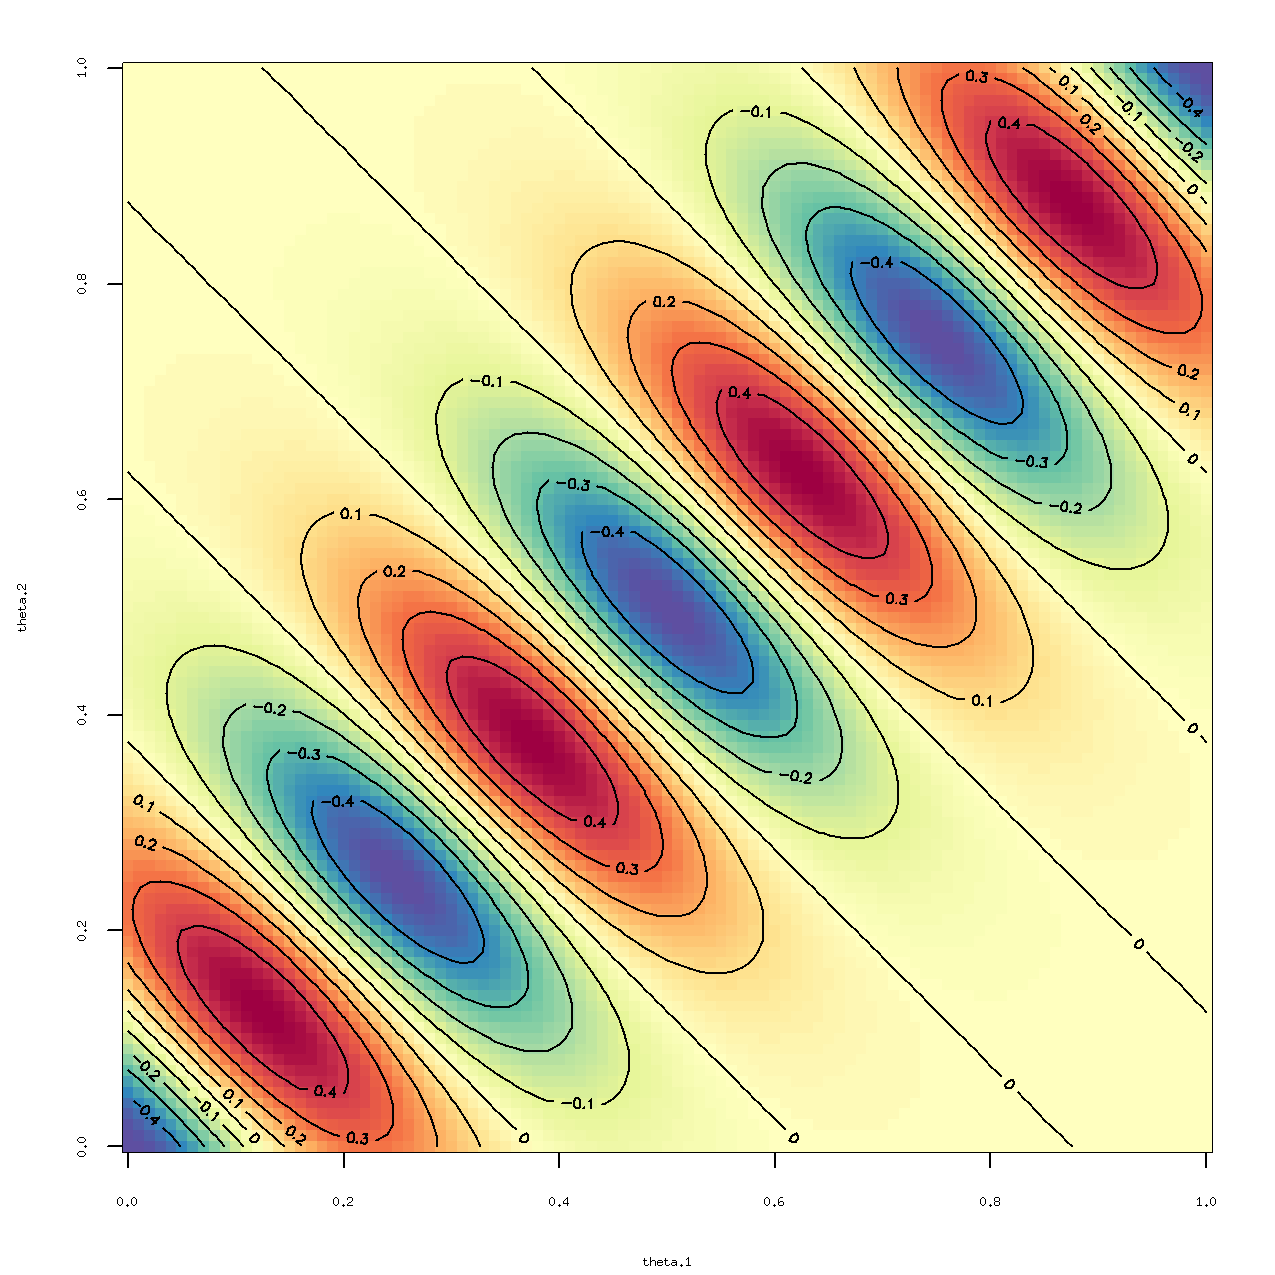
\includegraphics[width=0.24\linewidth]{figs/chap5/Diag4Max.png}
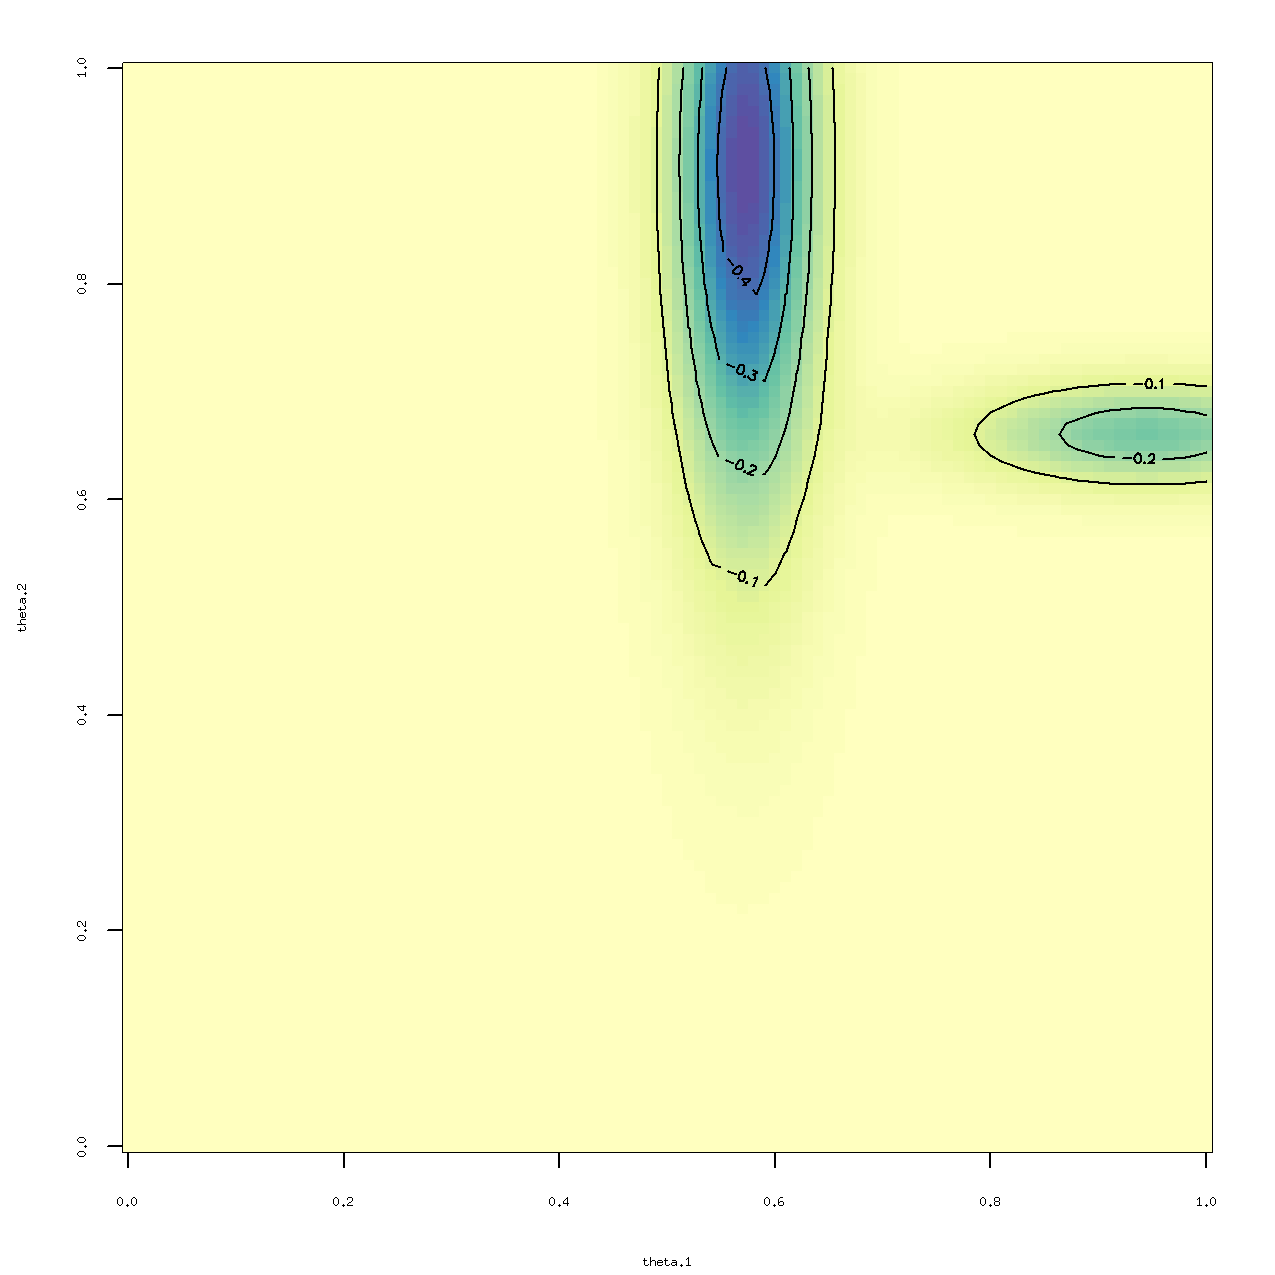
\includegraphics[width=0.24\linewidth]{figs/chap5/GMM2_2D.png}
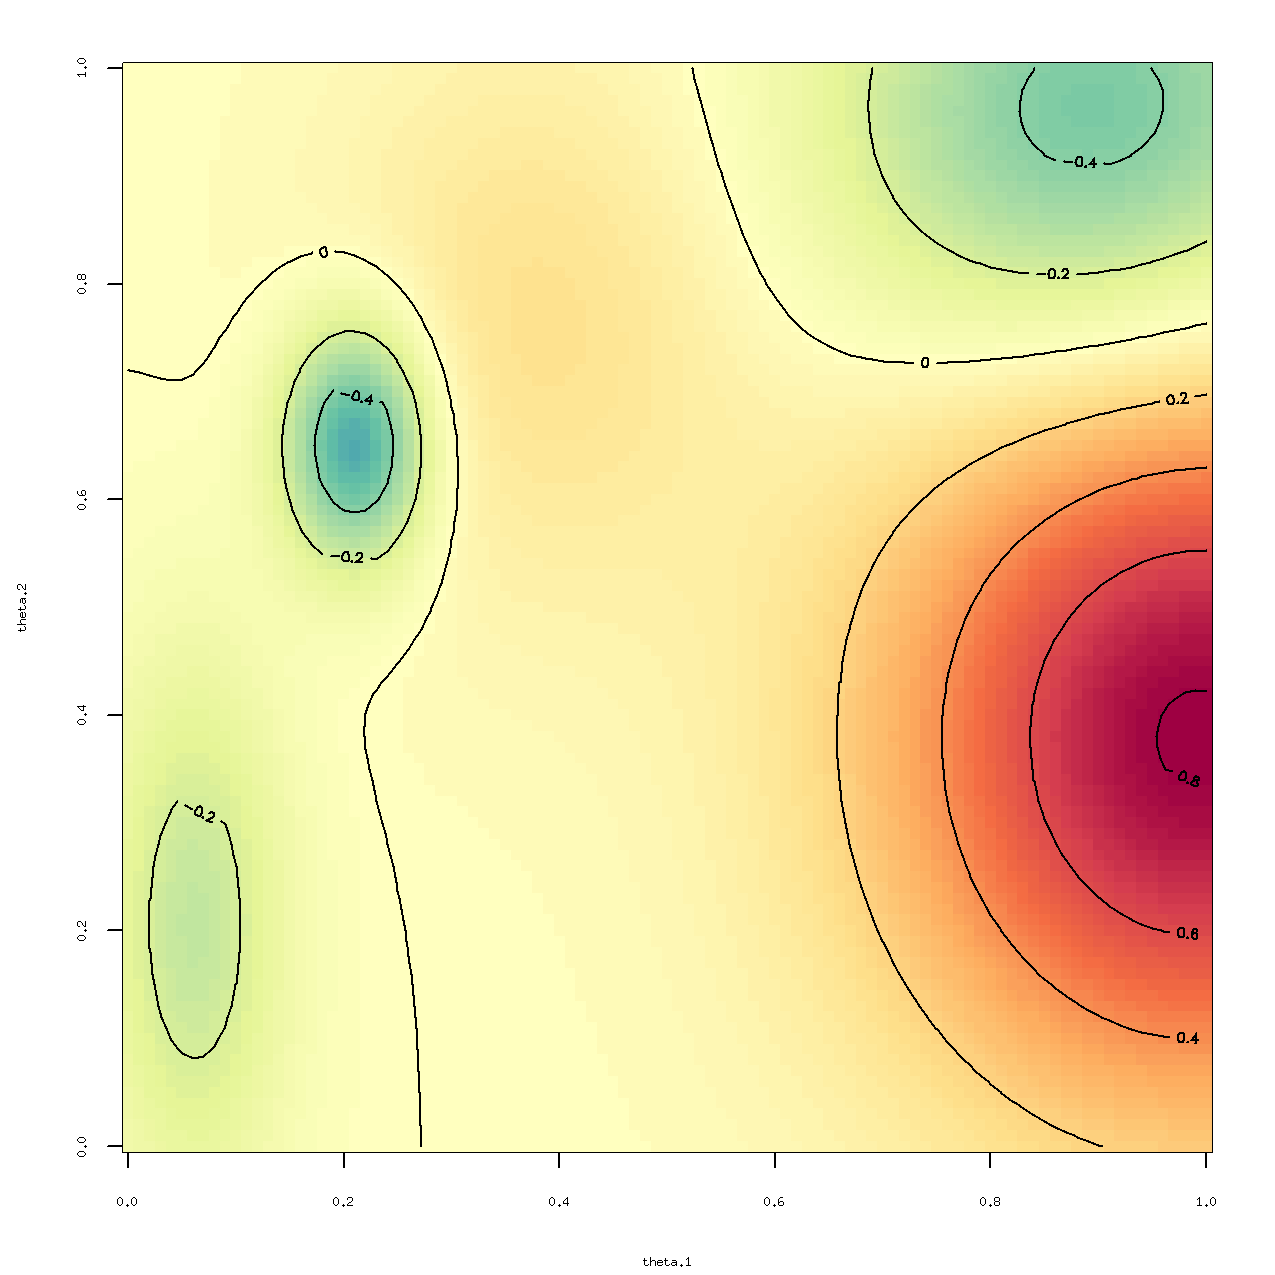
\includegraphics[width=0.24\linewidth]{figs/chap5/GMM5_2D.png}
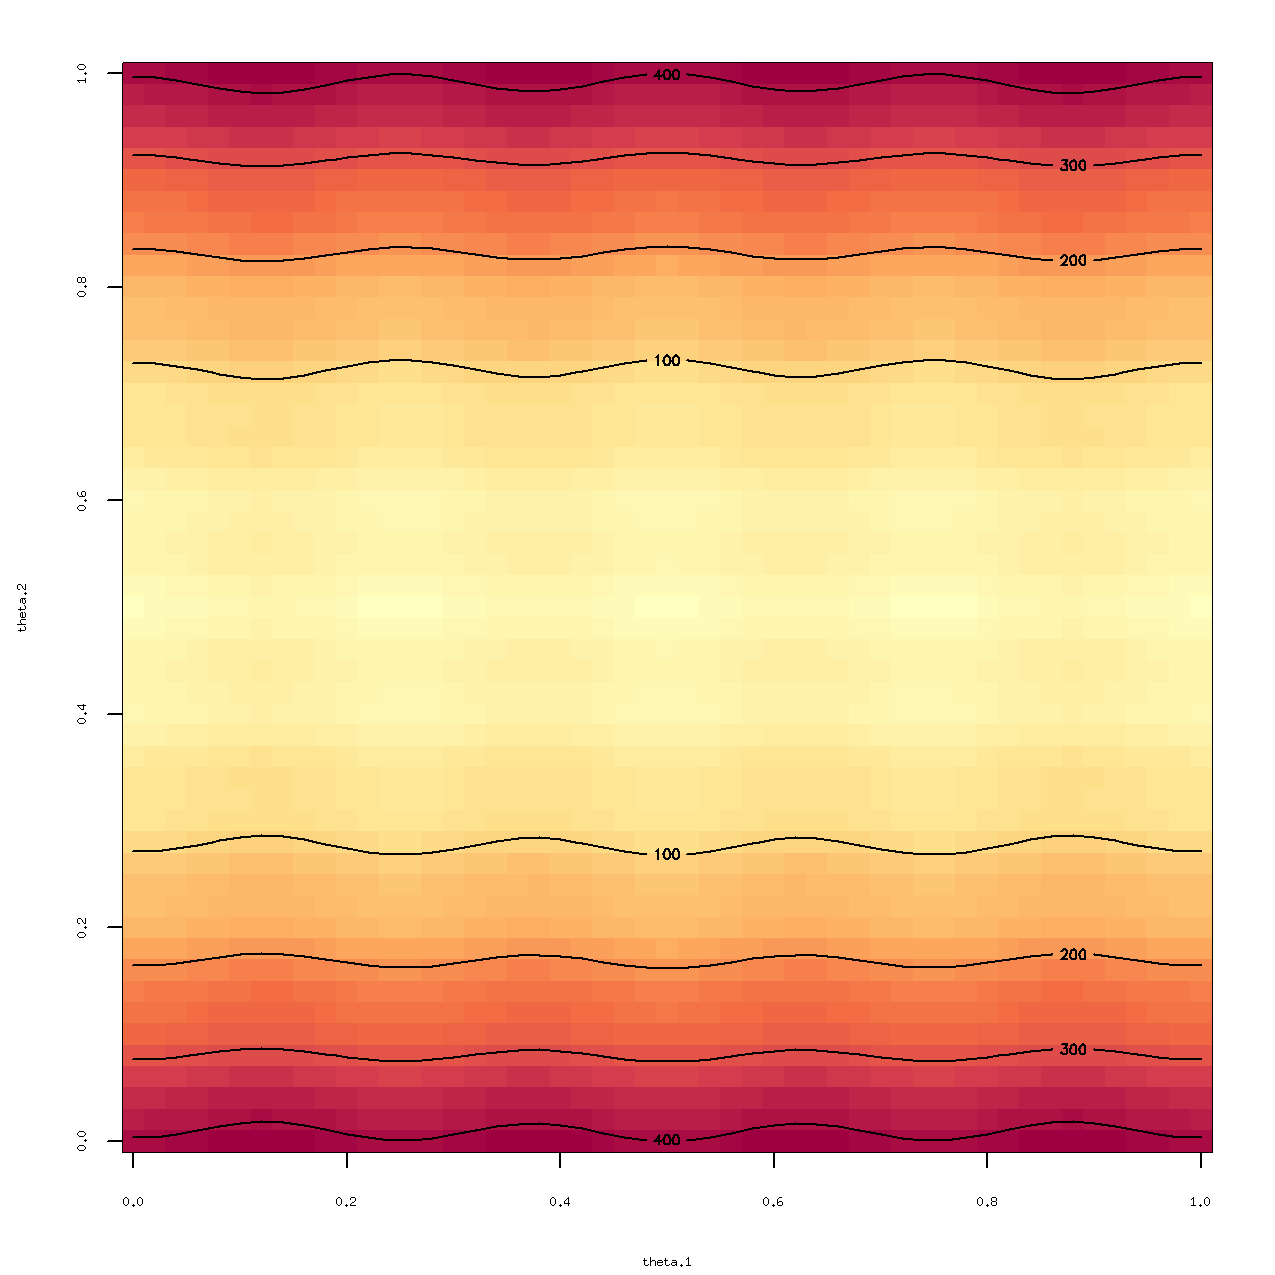
\includegraphics[width=0.24\linewidth]{figs/chap5/MGR.png}
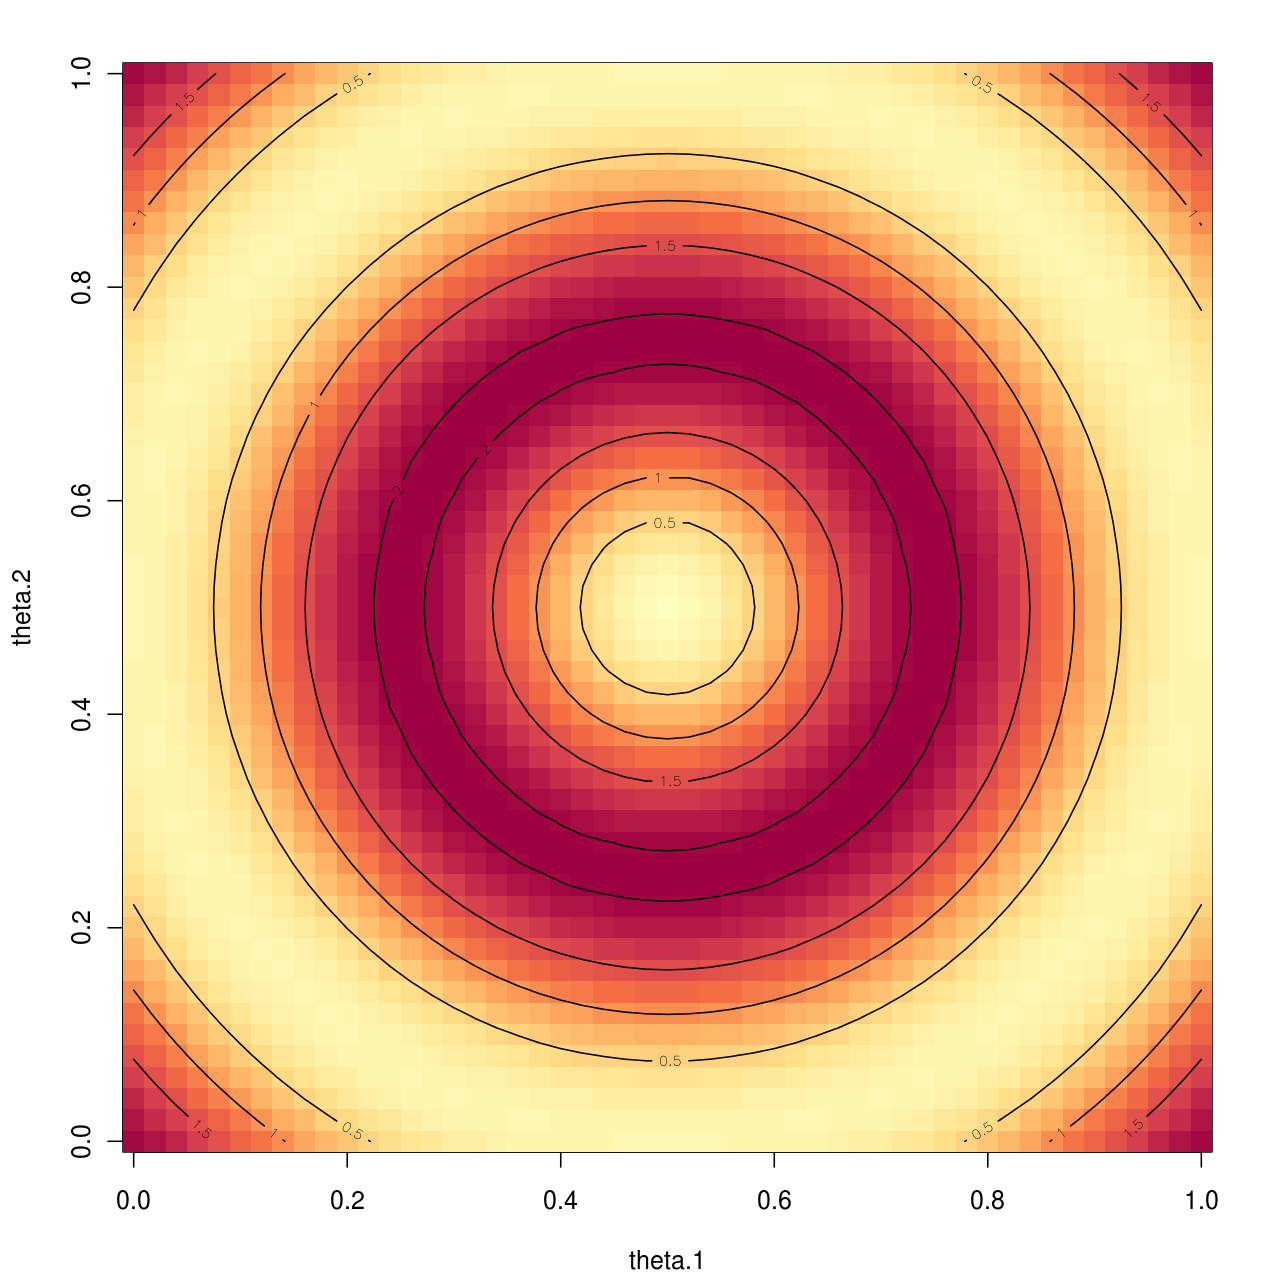
\includegraphics[width=0.24\linewidth]{figs/chap5/Salomon.png}
\includegraphics[width=0.24\linewidth]{figs/chap5/Whitley.png}
\caption{Pseudo-colored contour plots of the two-dimensional versions of the test functions.
%
From left to right: Ackley, diagonal function with two maxima (Diag2Max), diagonal function with four maxima (Diag4Max), Gaussian mixture model with two (GMM2) and five Gaussians (GMM5), Mis-scaled Generalized Rastrigin (MGR), Salomon and Whitley, respectively.}
\label{fig:original}
\end{center}
\end{figure}

We use several testing functions with closed forms described below.
%
All functions can be generalized to higher dimensions, and their two-dimensional contour plots are shown in Figure~\ref{fig:original}.
%
Let $D$ be the dimension of the input vector $\vec{\theta}$.


% \begin{table}[h!]
%   \begin{center}
%     \begin{tabular}{ | c | c | l | }
%       \hline \\
%       Name & Contour Plot & Equation \\
%       \hline \\
%       Ackley
%       &
%      \raisebox{-\totalheight}{\includegraphics[width=0.15\textwidth]{figs/Ackley.png}}
%       &
%       \(\displaystyle f(\vec{\theta}) = \sum_{i=1}^{D-1}\left(e^{-0.2}\sqrt{\theta_i^2+\theta_{i+1}^2} + 3(\cos(2\theta_i) + \sin(2\theta_{i+1}))\right), \) where $\{\vec{\theta}|\theta_i\in [-3,3]\}$. \\
%       \hline \\
%       Gaussian Mixture Model
%       &
%       \raisebox{-\totalheight}{\includegraphics[width=0.15\textwidth]{figs/GMM5_2D.png}}
%       &
%       Let $m$ be the number of extrema in the domain.
%       Let $a_i$ be the amplitude of the $i^{th}$ extrema.
%       Let $c_{i,j}$ be the $j^{th}$ coordinate of the $i^{th}$ extrema.
%       Let $\sigma_{i,j}$ be the standard deviation of the $i^{th}$ extrema with respect to the  $j^{th}$ coordinate.
%       \(
%       f(\vec{\theta}) = \sum_{i=1}^{m}\left(a_i e^{-\left(\sum_{j=1}^{D}\frac{\left(\theta_{i,j}-c_{i,j}\right)^2}{2\sigma_{i,j}^2}\right)}\right)\)
%       where $\{\vec{\theta}|\theta_i\in [0,1]\}$.
%       \hline
%       \end{tabular}
%       \caption{Test functions used}
%       \label{tbl:myLboro}
%   \end{center}
% \end{table}

\subsubsubsection{Ackley}
$$
f(\vec{\theta}) = \sum_{i=1}^{D-1}\left(e^{-0.2}\sqrt{\theta_i^2+\theta_{i+1}^2} + 3(\cos(2\theta_i) + \sin(2\theta_{i+1}))\right),
$$
where $\{\vec{\theta}|\theta_i\in [-3,3]\}$.

\subsubsubsection{Diagonal}
Let $m$ be the number of maxima along the main diagonal,
\begin{eqnarray*}
f(\vec{\theta}) = & \frac{1}{2}\sin\left(\pi\left(\frac{1}{2} + \left((m+1) \bmod{2}\right) + \frac{m\left(\sum_{i=1}^{D}\theta_i\right)}{D}\right)\right)
 \times e^{\left(\left(\sum_{i=1}^{D}\theta_i^2 -\frac{\left(\sum_{i=1}^{D}\theta_i\right)^2}{D}\right)\left(\frac{\log(0.001)}{\sqrt{D}}\right)\right)},
\end{eqnarray*}
where
$\{\vec{\theta}|\theta_i\in [-1,1]\}$.

\subsubsubsection{Random Gaussian Mixture Model}

Let $m$ be the number of extrema in the domain.
Let $a_i$ be the amplitude of the $i^{th}$ extrema.
Let $c_{i,j}$ be the $j^{th}$ coordinate of the $i^{th}$ extrema.
Let $\sigma_{i,j}$ be the standard deviation of the $i^{th}$ extrema with respect to the  $j^{th}$ coordinate.
$$
f(\vec{\theta}) = \sum_{i=1}^{m}\left(a_i e^{-\left(\sum_{j=1}^{D}\frac{\left(\theta_{i,j}-c_{i,j}\right)^2}{2\sigma_{i,j}^2}\right)}\right)
$$
where $\{\vec{\theta}|\theta_i\in [0,1]\}$.


\subsubsubsection{Mis-scaled Generalized Rastrigin}
$$
f(\vec{\theta}) = 10D + \sum_{i=1}^{D}\left((10^{\frac{i-1}{D-1}}\theta_i)^2 - 10\cos(2\pi(10^{\frac{i-1}{D-1}}\theta_i))\right)
$$
where
$\{\vec{\theta}|\theta_i\in [-2,2]\}$.


\subsubsubsection{Salomon}
$$
f(\vec{\theta}) = -\cos\left(2\pi\sum_{i=1}^D\theta_i^2\right) + 0.1\sqrt{\sum_{i=1}^D\theta_i^2} + 1
$$
where $\{\vec{\theta}|\theta_i\in [-1,1]\}$.

\subsubsubsection{Whitley}
$$
f(\vec{\theta}) = \sum_{i=1}^{D}\sum_{j=1}^{D}\left(\frac{k_{ij}^2}{4000} - cos(k_{ij}) + 1\right)
$$
where $\{\vec{\theta}|\theta_i\in [-1,2]\}$, and
$k_{ij} = (100(\theta_i^2-\theta_j)^2 + (1-\theta_j)^2)$.

\subsection{Software Packages and Parameter Settings}
\label{sec:package}

Now we give details on packages and parameter settings used in our experiments.

The GPM model we use is the \texttt{sparse online Gaussian process} (SOGP) C++ library \cite{gpm}, which is based on work in \cite{Csato2002,CsatoOpper2002}.
%
The default parameters are employed; see~\cite{CsatoOpper2002} for details.
%
In other words, we use the radial basis kernel with a spherical covariance set to $\sigma_0^2 = 0.1$, the widths are uniformly set to 0.1, and the amplitude $A=1$.

For EARTH, MDA and NNET, we use nonparametric bootstrapping using $250$ samples without cross-validation.

For EARTH, we use the \texttt{earth} library in \texttt{R} \cite{earth}.
%
We use the following parameter settings; see \cite{earth} for details.
%
If a parameter is not listed, the default value given by the package is used.
%
\begin{code}
degree=3 // Maximum degree of interaction (Friedman's mi)
nk=63  //Maximum number of model terms before pruning
minspan=1 //Min. dist. between knots, 1 for non-noisy data
thresh=1e-8  //Forward stepping threshold
penalty=3 //Generalized Cross Validation Penalty per knot
\end{code}

For MDA, we use \texttt{mda} library in \texttt{R}, with the following parameters (see \cite{mda} for details; nonlisted parameters use package defaults):
\begin{code}
degree=3 // Maximum degree of interaction (Friedman's mi)
nk=63  //Maximum number of model terms
thresh=1e-8 // Forward stepping threshold
penalty=3 // The cost per degree of freedom charge
\end{code}

For NNET, we use \texttt{nnet} library in \texttt{R}, with the following parameters (see \cite{nnet} for details; nonlisted parameters use package defaults):
\begin{code}
size=1+ceiling(sqrt(D)) // Number of units in the hidden layer
                        // D is the dimensionality of the input
decay=1e-3 // Parameter for weight decay
skip=TRUE // Add skip-layer connections from input to output
linout=TRUE // Linear output units, as opposed to logistic
\end{code}

To create the space-filling samplings, the \texttt{lhs} library in \texttt{R} \cite{lhs} is used.
%
More specifically, we use the \texttt{randomLHS} function, which chooses uniform, random samples without any attempts to optimize the design, to construct the training data, candidate data, and LHS samples in the plots shown.

%%%%%%%%%%%%%%%%%%%%%%%%%%%%%%%%%%%%%%%%%%%%%%%%%%%%%%%%%%%%%%%%%%%%%%%%%%%%%%%%
%%%%%%%%%%%%%%%%%%%%%%%%%%%%%%%%%%%%%%%%%%%%%%%%%%%%%%%%%%%%%%%%%%%%%%%%%%%%%%%%
%%%%%%%%%%%%%%%%%%%%%%%%%%%%%%%%%%%%%%%%%%%%%%%%%%%%%%%%%%%%%%%%%%%%%%%%%%%%%%%%

\section{Topology-Based Batch Sampling}
\label{paper:batch}

Section~\ref{paper:ijuq2013} focused on applying different scoring functions.
%
We now consider the problem of selecting multiple candidates at a time using various batch selection criteria for a fixed scoring function on two problem settings.
%
We again consider the problem of obtaining an accurate global fit, but in addition, we consider the problem of learning a limit surface.
%
In this second context, we are less concerned with the fit of our surrogate over the whole domain, but instead want to define the shape of a levelset for a single isovalue of the function under consideration.


\subsection{Batch Selection for Active Learning: General Pipeline}
The general pipeline of batch selection begins with a given set of training data with true response values.
%
First, a surrogate model is fit to the training data.
%
Second, a pool of candidate points is chosen in the domain based on a given sampling technique, typically a space-filling design that will not bias any particular area of the input domain.
%
Third, each candidate point is assigned a score.
%
Finally, a number of candidates (i.e., up to the batch size) with the highest scores are selected, evaluated (to obtain true response values), and added to the training data to begin a new round of fitting.
%
This pipeline is given in Algorithm~\ref{algo:al}, where we replace \textit{SELECT} with various selection strategies.
%
We use a sparse online Gaussian process~\cite{CsatoOpper2002} as the surrogate model.
%
For a given candidate, such a Gaussian process model gives a (mean) prediction value and a variance associated with the prediction.
%
The set of candidate points and the initial training data are selected using a centroidal Voronoi tessellation (CVT) sampling strategy~\cite{DuFaberGunzburger1999}.
%
A CVT sampling strategy gives high-quality samples without the biases introduced by a uniform grid sampling, although it can become cost prohibitive in high dimensions.
%
A Latin hypercube sampling (LHS)~\cite{ImanDavenportZeigler1980} strategy can be used for higher dimensional examples.
%
For each dataset, we measure the accuracy of our global or local fitting by comparing to the ground-truth at each iteration, under different metrics described in Section~\ref{sec:evaluation_metrics}.

As stated before, we consider two problems in this experiment, global fitting and limit surface extraction.
%
For the global surface recovery problem, we utilize the \emph{active learning MacKay} (ALM) scoring function~\cite{MacKay1992} presented in Section~\ref{sec:classic} that uses the predicted variance from the surrogate model as the score for a candidate point.
%
In this way, we reduce the overall uncertainty of the surrogate model by placing samples in the areas of the highest variance.

For the limit surface recovery problem, we utilize the \emph{straddle} scoring function~\cite{BryanSchneiderNichol2005}.
%
For a given candidate point, its score is formulated as a linear combination of the predicted variance and the distance between its predicted value and the limit surface threshold value.
%
In other words, a candidate will have a high score if its predicted value is near the limit surface threshold and/or it exhibits a large amount of prediction uncertainty.

{\fontsize{10}{10}\selectfont
\begin{algorithm}
\scriptsize
\caption{Batch selection for active learning}
\label{algo:al}
% \begin{spacing}{0.8}
\begin{algorithmic}
\INPUT {a set of training points, $T$}
\Statex{a set of candidate points, $C$}
\Statex{real-valued scoring function, $S(M,x)$, where $M$ is a surrogate model,
        $x$ is a point}
\Statex{real-valued true response function, $f(x)$, where $x$ is a point}
\Statex{batch size, $b$}
\OUTPUT{A surrogate model, $M(x)$, that evaluates at any point $x$}
\\
\While{$C \neq \emptyset$ and not converged}
  \State{$M \gets [T,f(T)]$}\Comment{Build a surrogate $M$ with the training
                                     data}
  \State{$ R \gets$ \textbf{SELECT}($C$, $S$, $M$, $b$) }\Comment{This is the step we will be augmenting}
  \State{$C \gets C \setminus R$}\Comment{Remove selected candidates}
  \State{$T \gets T \cup R$}\Comment{Add candidates to the training data}
\EndWhile
\end{algorithmic}
% \end{spacing}
\end{algorithm}
}

We now introduce the different specific methodologies for selecting a batch of candidates once the candidates have all been scored.

\subsection{Naive Batch Selection}
Batch selection is simple and straightforward when the batch size is $b = 1$.
%
We simply select the point with the highest score.
%
When $b>1$, it is not clear whether selecting the top $b$ highest scoring candidates is desirable.
%
For example, if the scoring function is based on predicted variance (e.g., active learning MacKay, ALM), the selected candidates may be clustered in a single area of high variance.
%
However, obtaining a single sample in that area would suffice to reduce the uncertainty for the whole area.
%
Nonetheless, we use this naive strategy as a baseline, and its corresponding algorithm is given in Algorithm \ref{algo:naive}.

{\fontsize{10}{10}\selectfont
\begin{algorithm}
\scriptsize
\caption{Naive batch selection}
\label{algo:naive}
% \begin{spacing}{0.8}
\begin{algorithmic}
\Procedure{\textbf{Naive-Select}}{$C, S, M, b$}
  \State $R \gets \emptyset$
  \While{$|R| \neq b$}
  \State{$\widetilde{C} = C \setminus R$}
  %\State{find $p \in \widetilde{C}$ s.t. $S(M,p) = \max(S(M,\widetilde{C})$)}
  \State $p^* = \argmax{p \in \widetilde{C}} S(M, p)$
  \State{$R \gets R \cup p^*$}
  \EndWhile
  \State return $R$
\EndProcedure
\end{algorithmic}
% \end{spacing}
\end{algorithm}
}

\subsection{Surrogate Believer Batch Selection}
This strategy is inspired by the Kriging believer strategy~\cite{GotovosCasatiHitz2013,GinsbourgerLeRicheCarraro2009}.
%
It takes advantage of the scoring function's reliance on the uncertainty of the surrogate model.
%
The main idea is that temporarily adding a point and its model-predicted response value to refit (update) the surrogate model will not drastically alter the response surface, but it will reduce the variance in the area surrounding this point.
%
As both scoring functions used are variance-based, re-scoring the candidates based on the updated surrogate model would likely cause the new highest scoring candidate to be farther away from the last selected point.
%
Formally, this process is described in Algorithm \ref{algo:believe}, where $M(x)$ returns the predicted response value using the surrogate model at point(s) $x$.

{\fontsize{10}{10}\selectfont
\begin{algorithm}
\scriptsize
\caption{Believer batch selection}
\label{algo:believe}
% \begin{spacing}{0.8}
\begin{algorithmic}
\Procedure{\textbf{Believer-Select}}{$C, S, M, b$}
\State{$R \gets \emptyset$}
\While{$|R| \neq b$}
  \State{$\widetilde{C} = C \setminus R$}
  \State{$\widetilde{M} \gets M + [R,M(R)]$}
  \LineComment{Build a temporary surrogate model that treats $R$ and $M(R)$ as
               part of the training set}
  %\State{find $p \in \widetilde{C}$ s.t. $S(\widetilde{M},p) = \max(S(\widetilde{M},\widetilde{C})$)}
  \State $p^* = \argmax{p \in \widetilde{C}} S(\widetilde{M}, p)$
  \State{$R \gets R \cup p^*$}
\EndWhile
\State return $R$
\EndProcedure
\end{algorithmic}
% \end{spacing}
\end{algorithm}
}

\subsection{Topology-Based Batch Selection: Points with\\Maximum Persistence}
\label{subsection:topology-maxp}

We now utilize the topological method described earlier to study the topology of the scoring function.
%
Scoring function $S$ is a real-valued function that takes as input a surrogate model $M$ and a point $x$, and returns a real number based on properties of $M$, the predicted value $M(x)$, the variance of the prediction, etc.
%
When $b = 1$, the naive strategy always selects the highest scoring candidate, which, topologically, corresponds to the global maximum of the scoring function.
%
When $b > 1$, the naive strategy selects $b$ points with the highest scores, and does not guarantee good spacing among the selected candidates since these points may cluster around the global maxima.
%
If we would like to guarantee some level of spatial separation among the chosen candidates, then perhaps a simple topology-based strategy would select the top $b$ \emph{local maxima} of the scoring function.
%
However, as the example illustrated in Figure~\ref{fig:persistence} shows, a 1D scoring function could contain two local maxima that are close to each another in the domain but have very different \emph{persistence}.
%
Such an observation inspired our first topology-based batch selection strategy, which is based on the persistence of the candidate points.
%
Since regular points have zero persistence, such a strategy selects points exclusively among the local maxima.
%
That is, we select the top $b$ candidates with the highest persistence.
%
This strategy is detailed in Algorithm \ref{algo:maxp}.

{\fontsize{10}{10}\selectfont
\begin{algorithm}
\scriptsize
\caption{Maximum persistence batch selection}
\label{algo:maxp}
% \begin{spacing}{0.8}
\begin{algorithmic}
\Procedure{\textbf{MaxP-Select}}{$C, S, M, b$}
\State{$R \gets \emptyset$}
\State{$X \gets$ \textbf{EXTRACT-LOCAL-MAXIMA}($C,S,M$)}
\LineComment{Extract all local maxima from the scoring function of the surrogate
             model}
%\Comment{See section \ref{topology} for details}
\While{$|X| < b$}
\LineComment{While loop is only used if we do not have $b$ unselected local
             maxima}
  \State{$\widetilde{C} = C \setminus X$}
  %\State{find $p \in \widetilde{C}$ s.t. $S(\widetilde{M},p) = \max(S(\widetilde{M},\widetilde{C})$)}
  \State $p^* = \argmax{p \in \widetilde{C}} S(M, p)$
  \State{$X \gets X \cup p^*$}
\EndWhile
\State{$R \gets R \cup \textbf{TOP}(X,b)$}\Comment{Get only the top $b$ maxima
                                                   (according to persistence)}
\State return $R$
\EndProcedure
\end{algorithmic}
% \end{spacing}
\end{algorithm}
}

Since we would like to generalize our batch selection process to any arbitrary dimension, we compute an approximated Morse complex of the scoring function using the algorithm from Section~\ref{sec:approximationMSC} to estimate the location of its local maxima and their corresponding persistence.

\begin{figure}[!ht]
\centering
\includegraphics[width=0.32\textwidth]{figs/chap5/persistence}
\includegraphics[width=0.32\textwidth]{figs/chap5/persistence2}
\caption{A simple one-dimensional function with four maxima showing a selection strategy that chooses the two highest-valued maxima (left) and the strategy we employ in MaxP, which selects the two highest persistence maxima.}
\label{fig:persistence}
\end{figure}

\subsection{Topology-Based Batch Selection:\\Maximum Persistence and Believer Hybrid}
Our final strategy creates a hybrid between the maximum persistence strategy and the surrogate believer strategy.
%
That is, we proceed with the believer strategy by temporarily adding points with the highest persistence.
%
We introduce one extra parameter $m$ that indicates how many points we add temporarily at the same time.
%
Equivalently, $m$ means the number of maxima to chose before refitting the surrogate.
%
$m=1$ corresponds to the original believer strategy, and $m = b$ corresponds to the maximum persistence strategy.
%
For all other values in between, $1 < m < b$, we blend the two ideas together.
%
The process is detailed in Algorithm \ref{algo:maxp-believe}.

{\fontsize{10}{10}\selectfont
\begin{algorithm}
\scriptsize
\caption{Maximum persistence and believer hybrid selection}
\label{algo:maxp-believe}
% \begin{spacing}{0.8}
\begin{algorithmic}
\Procedure{\textbf{MaxP+Believe-Select}}{$C, S, M, b$, (optional) $m$}
\State{$R \gets \emptyset$}
\While{$|R| \neq b$}
  \State{$\widetilde{C} = C \setminus R$}
  \State{$\widetilde{M} \gets M \cup [R,M(R)]$}
  \State{$X \gets$ \textbf{EXTRACT-LOCAL-MAXIMA}($\widetilde{C},S,\widetilde{M}$)}
  \LineComment{Extract all local maxima from the scoring function of the
               temporary surrogate model}
  %\Comment{See section \ref{topology} for details}
  \State{$X \gets X \setminus R$}
  \LineComment{Remove any local maxima that have already been selected}
  \While{$|X| < m$}
  \LineComment{While loop is only used if we do not have $m$ unselected local
               maxima}
    \State{$\widetilde{C} = \widetilde{C} \setminus X$}
    %\State{find $p \in \widetilde{C}$ s.t. $S(\widetilde{M},p) = \max(S(\widetilde{M},\widetilde{C})$)}
    \State $p^* = \argmax{p \in \widetilde{C}} S(\widetilde{M}, p)$
    \State{$X \gets X \cup p^*$}
  \EndWhile
  \State{$R \gets R \cup \textbf{TOP}(X,m)$}\Comment{Get only the top $m$ maxima
                                                     (according to persistence)}
\EndWhile
\State return $R$
\EndProcedure
\end{algorithmic}
% \end{spacing}
\end{algorithm}
}

\subsection{Evaluation Metrics}
\label{sec:evaluation_metrics}
%
For the global surface recovery problem, we compute the \emph{root-mean-square error} (RMSE) over a validation set $V$ of the domain between the surrogate model response surface and the true response surface.
%
The validation set $V$ for our two-dimensional test functions is a uniform grid of resolution $100\times100$.

For the limit surface recovery problem, we use two metrics to try to quantify the quality of the approximations.
%
The \emph{Hausdorff distance} between the true limit surface and the approximated limit surface based on the surrogate model is computed to measure curve similarity.
%
This metric represents the maximum separation of the two limit surfaces represented as point set samples $X$ and $Y$. It is defined as:

\begin{equation}
d_H(X,Y) = \max \left( \sup_{x \in X} \inf_{y \in Y}
d(x,y),\sup_{y \in Y} \inf_{x \in X} d(x,y)\right).
\end{equation}

In addition, we treat our model as a binary classifier with the limit surface being the boundary and compute the \emph{$F_1$-score}.
%
Given a ground-truth validation grid, we can evaluate the \emph{precision}, $p$, and \emph{recall}, $r$, of the classification and compute the harmonic mean of these two values to get the $F_1$-score.
%
The relevant equations are listed below, where $t_+$ means the count of `true positives' or correctly identified labels above the limit surface, $f_+$ means the count of `false positives' or incorrectly identified labels above the limit surface, and $f_-$ means the count of `false negatives' or incorrectly identified labels below the limit surface.

\begin{equation}
p = \frac{t_+}{t_+ + f_+}
\end{equation}

\begin{equation}
r = \frac{t_+}{t_+ + f_-}
\end{equation}

\begin{equation}
F_1 = \frac{2pr}{p+r}
\end{equation}


The \emph{$F_1$-score} demonstrates the surrogate model's ability to correctly classify points as being either above or below the threshold value.
%
It is evaluated on a validation grid of resolution $100\times100$.
%
The Hausdorff distance focuses on the approximation quality of the limit surface itself.
%
Consider a small component of the limit surface that is yet to be recovered.
%
The F1-score may still report a high-value (corresponding to good approximation quality) since the missing component encloses only a small area of the domain space, but the Hausdorff distance may be very large (corresponding to a low approximation quality) because not all components in the limit surface have been recovered.

In other words, the Hausdorff distance metric complements the F1-score metric, since the former is a shape-matching criterion and the latter focuses on classification accuracy.
%
% Thus, yielding one shape-based metric and another volume-based metric.

\subsubsection{Test Functions}
We first use a collection of two-dimensional synthetic functions (with closed-form expressions) as test functions.
%
Since these functions are simple, smooth and continuous, the surrogate models on them converge very quickly during the active learning process.
%
We demonstrate that our methods remain competitive on these functions, where intuitively they are not expected to perform as well since the main features will be recovered quickly and will benefit more from exploitation rather than exploration.
%
In addition, these functions have well-defined, smooth limit surfaces that can be recovered accurately and efficiently, ensuring good convergence qualities of all methods.
%
We include three test functions here.
%
We omit their closed-form expressions but illustrate the smooth functions (true response surfaces) in Figure~\ref{fig:synthetic}(a)-(c).
%
Their corresponding limit surfaces (marked by yellow curves) are shown in Figure~\ref{fig:synthetic}(d)-(f).
%
The GMM corresponds to the surface of a two-dimensional Gaussian mixture model.
%
The GMM has three limit surface components with one designed to be smaller and less likely to be found immediately.
%
The limit surface of the Salomon function contains three concentric rings, where the outermost ring is split into four components due to the selected boundary location.
%
The Sinusoidal function has a relatively complex limit surface with multiple components, but spans a large portion of the domain.
%Thus, one might expect a faster Hausdorff convergence on the Sinusoidal
%function than the GMM, but the  $F_1$-score ...nevermind

\begin{figure}[!ht]
\centering
\includegraphics[width=0.98\textwidth]{figs/chap5/synthetic}
\caption{Synthetic test functions and their designated limit surfaces.
(a)-(c): True response surfaces for (a) GMM, (b) Salomon and (c) Sinusoidal.
(d)-(f): True limit surfaces for (d) GMM, (e) Salomon and (f) Sinusoidal.}
\label{fig:synthetic}
\end{figure}

To demonstrate that our proposed topology-based active learning methods can potentially be more advantageous with functions that have complex topology, we use a set of grayscale images as our real-world test functions.
%
We treat each image as a two-dimensional function, where its domain is defined by the pixel locations and its range is the luminosity ranging between $0$ (black) to $255$ (white).
%
The images we have selected contain irregular shapes, discontinuities, and noisy features, which are more indicative of real-world data.
%
They are shown with superimposed limit surfaces in Figure~\ref{fig:images}.
%
The limit surfaces are highly irregular with many small components, and their corresponding threshold values are $125$, $30$, $80$, and $100$, respectively.

\begin{figure}[b]
\centering
\includegraphics[width=0.98\textwidth]{figs/chap5/images}
\caption{Test images. True limit surfaces are marked with yellow curves.
%
(a) Face.
%
(b) Butterfly nebula (image courtesy of NASA, ESA and the Hubble SM4 ERO Team,
in public domain, via Wikimedia Commons).
%
(c) Tiger (image courtesy of Wikimedia Commons).
%
(d) Valve (image courtesy of Wikimedia Commons).}
\label{fig:images}
\end{figure}

\subsection{Results for Global Surface Recovery}
\label{sec:global_results}
%
% \paragraph{RMSE Convergence Results.}
Table \ref{table:global-synthetic} summarizes the number of points necessary to reduce the global RMSE under a given threshold for each test function.
%
The threshold value is chosen by examining the RMSE convergence across all trials, e.g., we stop the active learning process when RMSE falls below $0.07818$ for the GMM dataset.
%
We report the mean number of points required as well as the standard deviation for each strategy across $10$ trials.
%
The numbers in parentheses are the median values across each of the $10$ trials.
%
The maximum number of points added for the synthetic test functions is capped at $256$ and for the image datasets, at $1024$.
%
We experiment with three different batch sizes, $8$, $16$, and $32$.
%
We adopt shorthand for each strategy in the following tables; for example, 2-MaxP+Believe means the hybrid strategy where the parameter $m = 2$.
%
The strategy with the best performance for each dataset is highlighted in bold font.
%
If the best strategy is topology-based, it is colored in red.

\begin{table}[t]
\scriptsize
\centering
\begin{tabular}{l || c | c | c}
   & GMM  & Salomon  & Sinusoidal \\
  &  ( $\leq$ 0.07818 )  &  ( $\leq$ 0.07169 )  &  ( $\leq$ 0.04674 ) \\
\hline\hline
($b=8$)  &   &   &  \\
\hline
Naive            & 120.8 $\pm$ 28.72 (108)        & 152.8 $\pm$ 13.12 (152)        & 132.0 $\pm$ 8.198 (128)\\
Believe          & 52.8 $\pm$ 9.6 (52)            & \textbf{91.2 $\pm$ 3.919 (88)} & \textbf{68.0 $\pm$ 4.0 (68)} \\
MaxP             & 56.0 $\pm$ 8.0  (56)           & 93.6 $\pm$ 3.666 (96)          & 75.2 $\pm$ 5.307 (76)\\
2-MaxP + Believe & \myemph{52.0 $\pm$ 9.633 (48)} & 93.6 $\pm$ 5.122 (96)          & 68.8 $\pm$ 3.919 (72)\\
4-MaxP + Believe & 56.8 $\pm$ 15.37 (52)          & 94.4 $\pm$ 3.2 (96)            & 70.4 $\pm$ 4.8 (72)\\
\hline\hline
 ($b=16$)  &    &    &   \\
\hline
Naive            & 169.6 $\pm$ 36.63 (160)        & 203.2 $\pm$ 12.5 (200)     & 190.4 $\pm$ 16.7 (192)\\
Believe          & 59.2 $\pm$ 14.4 (56)           & \textbf{96.0 $\pm$ 0 (96)} & \textbf{72.0 $\pm$ 8.0 (72)} \\
MaxP             & 60.8 $\pm$ 9.6 (64)            & 105.6 $\pm$ 7.838 (112)    & 84.8 $\pm$ 7.332 (80)\\
2-MaxP + Believe & \myemph{57.6 $\pm$ 14.66 (48)} & 97.6 $\pm$ 4.8 (96)        & 73.6 $\pm$ 7.838 (80)\\
4-MaxP + Believe & 60.8 $\pm$ 15.68 (56)          & \myemph{96.0 $\pm$ 0 (96)} & 75.2 $\pm$ 7.332 (80)\\
\hline\hline
 ($b=32$)  &    &    &   \\
\hline
Naive            & 192.0 $\pm$ 28.62 (192)      & 243.2 $\pm$ 15.68 (256)    & 249.6 $\pm$ 12.8 (256)\\
Believe          & \textbf{67.2 $\pm$ 9.6 (64)} & \textbf{96.0 $\pm$ 0 (96)} & \textbf{80.0 $\pm$ 16.0 (80)} \\
MaxP             & 99.2 $\pm$ 17.23 (96)        & 140.8 $\pm$ 15.68 (128)    & 124.8 $\pm$ 9.6 (128)\\
2-MaxP + Believe & \myemph{67.2 $\pm$ 9.6 (64)} & 99.2 $\pm$ 9.6 (96)        & 83.2 $\pm$ 15.68 (96)\\
4-MaxP + Believe & 70.4 $\pm$ 12.8 (64)         & \myemph{96.0 $\pm$ 0 (96)} & 86.4 $\pm$ 14.66 (96)\\
\end{tabular}
\caption{RMSE convergence results for synthetic test functions.}
\label{table:global-synthetic}
\end{table}

Increasing the batch size $b$ decreases the rate of convergence, since refitting the surrogate more frequently with small batch sizes would likely select more informative samples.
%
The naive method typically gives a baseline performance that is much worse than all other methods, but it shows the range of performance values and illustrates that the believe, MaxP, and their hybrid strategies are competitive with one another with respect to the overall range.
%
On these smooth, relatively simple surfaces, the results shown here slightly favor the believe strategy, in most cases.
%
The MaxP strategy degrades poorly when increasing the batch size from $16$ to $32$, most likely due to the fact that there are likely less than $32$ local maxima extracted from the ALM scoring function.
%
When all the local maxima have been selected, the remaining candidates are chosen based on the naive method.
%
By coupling the MaxP strategy with the believe strategy, we see relatively good performances across many scenarios, since such a hybrid strategy takes advantage of exploiting the topology of the scoring functions.

\begin{table}[h]
\scriptsize
\centering
\begin{tabular}{l || c | c | c | c }
   & Face  & Nebula  & Tiger  & Valve \\
  &  ( $\leq$ 29.83 )  &  ( $\leq$ 19.8 )  &  ( $\leq$ 51.94 )  &  ( $\leq$ 38.52 ) \\
\hline\hline
($b=8$)  &   &   &   &  \\
\hline
 Naive            & 776.0 $\pm$ 69.47 (768)          & 770.4 $\pm$ 96.8 (748)           & 766.4 $\pm$ 48.77 (768)          & 683.2 $\pm$ 71.3 (680) \\
 Believe          & \textbf{755.2 $\pm$ 56.02 (772)} & 626.4 $\pm$ 112.7 (640)          & 732.0 $\pm$ 97.6 (728)           & 619.2 $\pm$ 99.1 (604)\\
 MaxP             & 796.0 $\pm$ 51.75 (800)          & 624.0 $\pm$ 109.5 (596)          & \myemph{721.6 $\pm$ 125.9 (704)} & 628.8 $\pm$ 72.99 (632) \\
 2-MaxP + Believe & 749.6 $\pm$ 54.73 (744)          & 680.0 $\pm$ 49.19 (676)          & 792.8 $\pm$ 113.1 (816)          & \myemph{581.6 $\pm$ 97.33 (588)} \\
 4-MaxP + Believe & 756.8 $\pm$ 50.87 (764)          & \myemph{603.2 $\pm$ 106.7 (616)} & 777.6 $\pm$ 90.85 (780)          & 608.8 $\pm$ 94.42 (620) \\
\hline\hline
 ($b=16$)  &    &    &    &   \\
Naive             &  832.0 $\pm$ 91.63 (816)          & 872.0 $\pm$ 98.95 (864)          & 772.8 $\pm$ 121.4 (792)          & 756.8 $\pm$ 58.15 (760) \\
Believe           &  \textbf{756.8 $\pm$ 58.15 (776)} & 630.4 $\pm$ 111.1 (640)          & \textbf{732.8 $\pm$ 90.45 (712)} & 630.4 $\pm$ 98.16 (632)\\
MaxP              &  820.8 $\pm$ 20.3 (816)           & 656.0 $\pm$ 115.2 (648)          & 737.6 $\pm$ 149.3 (800)          & 595.2 $\pm$ 87.87 (576)\\
2-MaxP + Believe  &  779.2 $\pm$ 70.85 (768)          & 688.0 $\pm$ 66.74 (680)          & 788.8 $\pm$ 109.5 (784)          & 600.0 $\pm$ 93.91 (592)\\
4-MaxP + Believe  &  768.0 $\pm$ 73.67 (776)          & \myemph{617.6 $\pm$ 85.33 (680)} & 737.6 $\pm$ 97.97 (736)          & \myemph{590.4 $\pm$ 98.49 (592)} \\
\hline\hline
 ($b=32$)  &    &    &    &   \\
\hline
Naive            & 918.4 $\pm$ 84.72 (944)          & 953.6 $\pm$ 69.82 (992)          & 825.6 $\pm$ 112.5 (800)          & 838.4 $\pm$ 86.81 (848)\\
Believe          & 768.0 $\pm$ 68.63 (784)          & \textbf{608.0 $\pm$ 108.0 (640)} & \textbf{761.6 $\pm$ 99.97 (768)} & 640.0 $\pm$ 90.51 (640)\\
MaxP             & 828.8 $\pm$ 36.35 (832)          & 742.4 $\pm$ 104.0 (736)          & 832.0 $\pm$ 91.63 (832)          & \myemph{617.6 $\pm$ 111.8 (576)} \\
2-MaxP + Believe & 787.2 $\pm$ 32.63 (784)          & 739.2 $\pm$ 103.6 (704)          & 806.4 $\pm$ 129.4 (784)          & \myemph{617.6 $\pm$ 116.3 (608)} \\
4-MaxP + Believe & \myemph{761.6 $\pm$ 49.16 (768)} & 656.0 $\pm$ 90.79 (608)          & 803.2 $\pm$ 84.0 (800)           & 630.4 $\pm$ 79.74 (640)\\
\end{tabular}
\caption{RMSE convergence results for image datasets.}
\label{table:global-images}
\end{table}

The results for the image datasets are shown in Table \ref{table:global-images}.
%
These datasets exhibit more complicated convergence behaviors.
%
They require more relaxed RMSE convergence thresholds and a larger number of samples to reach even modest levels of approximation.
%
In the case of the butterfly nebula image and the tiger image when $b=8$, the MaxP method outperforms the believe strategy.
%
In many other cases, the hybrid strategies have the best performance in terms of mean values.
%Meanwhile, the reported standard deviations are rather large, putting most
%scenarios within the same range of one another.

\subsection{Results for Limit Surface Recovery}
\label{sec:limit_results}
We discuss results for limit surface recovery in this section.
%
First, to understand the difference between the believe strategy and the topology-based MaxP strategy, we show some snapshots of the predicted response surfaces, as well as the corresponding scoring landscapes  (i.e. straddle) during the active learning process in Figure~\ref{fig:exampleLimits}, when $152$ candidates have already been added to the original $100$ training points.
%
The yellow contours denote the predicted limit surface.
%
The blue points are the training data (the same for both trials) and the red points are the adaptively selected points.
%
The green points represent the next batch of eight selected points.
%
The most important observation is that the believe strategy can still select points clustered in a single region, potentially limiting the amount of information gain from a single batch, as illustrated by the points enclosed in the white circles in Figure~\ref{fig:exampleLimits}(a)-(b).
%
The reason for this behavior is due in part to the straddle function encoding both uncertainty (in the form of variance) and closeness between the predicted value and the limiting surface threshold.
%
Recall the advantage of an adaptive sampling strategy over a space-filling design is that samples can be sequentially chosen in a proportionately small area of interest.
%
However, we emphasize that our purpose of using batch selection is to explore different areas simultaneously.
%
We believe our topology-based designs are more advantageous in such a context, as illustrated in Figure~\ref{fig:exampleLimits}(c)-(d), where the (green) points selected are well spaced from one another, capturing structural information from different areas of the domain.

\begin{figure}[!ht]
\centering
\includegraphics[width=0.98\textwidth]{figs/chap5/example-limits}
\caption{(a)-(b): (a) Predicted response surface based on surrogate model using
the believe strategy and (b) its corresponding scoring function.
%
(c)-(d): (c) Predicted response surface based on MaxP strategy and (d) its
corresponding scoring function.}
\label{fig:exampleLimits}
\end{figure}

\subsubsection{F1-Score Convergence Results.}
Treating the limit surface recovery problem as a binary classification, the F1-score can be used to understand our model's ability to correctly classify points.
%
Table \ref{table:f1_synthetics} presents the convergence results.
%The convergence threshold is chosen by comparing the convergence plots of each
%strategy on each test function.
%A maximum of $256$ points are added for the synthetic functions, and $1024$
%points are added for the image datasets.
For these synthetic functions, the majority of tests favor the believe strategy, most likely because on such simple and smooth examples, there is little need to explore the global space after a few rounds of sampling, and exploiting around the identified limit surface areas is more advantageous.
%
As the topology-based methods are believed to be more judicious about not placing samples very close to one another, they will not converge as quickly as the pure believe strategy, which can select clusters of points.

\begin{table}[t]
\scriptsize
\centering
\begin{tabular}{l || c | c | c }
 & GMM & Salomon & Sinusoidal \\
 & ( $\leq$ 0.9871 ) & ( $\leq$ 0.988 ) & ( $\leq$ 0.9942 ) \\
\hline\hline
 ($b=8$) & & & \\
\hline
 Naive            & 114.4 $\pm$ 12.42 (112)        & 158.4 $\pm$ 16.7 (156)           &  148.0 $\pm$ 26.59 (140) \\
 Believe          & \textbf{60.0 $\pm$ 9.633 (64)} & \textbf{120.8 $\pm$ 14.51 (120)} & \textbf{104.0 $\pm$ 13.86 (96)} \\
 MaxP             & 69.6 $\pm$ 10.15 (64)          & 142.4 $\pm$ 18.52 (140)          &  116.8 $\pm$ 18.66 (116) \\
 2-MaxP + Believe & \myemph{60.0 $\pm$ 8.198 (60)} & 142.4 $\pm$ 14.22 (148)          & 116.0 $\pm$ 19.02 (112) \\
 4-MaxP + Believe & 67.2 $\pm$ 5.307 (68)          & 144.0 $\pm$ 14.31 (144)          &  125.6 $\pm$ 19.61 (128) \\
\hline\hline
 ($b=16$) & & & \\
 Naive            & 168.0 $\pm$ 21.76 (168)        & 195.2 $\pm$ 15.68 (192)          &  176.0 $\pm$ 25.8 (176) \\
 Believe          & 67.2 $\pm$ 6.4 (64)            & \textbf{126.4 $\pm$ 15.09 (128)} & \textbf{107.2 $\pm$ 26.82 (96)} \\
 MaxP             & 81.6 $\pm$ 11.2 (80)           & 137.6 $\pm$ 10.61 (136)          & 116.8 $\pm$ 17.6  (112)\\
 2-MaxP + Believe & \myemph{64.0 $\pm$ 7.155 (64)} & 129.6 $\pm$ 8.616 (128)          & 108.8 $\pm$ 17.23 (112)\\
 4-MaxP + Believe & 70.4 $\pm$ 7.838 (64)          & 137.6 $\pm$ 16.32 (128)          & 116.8 $\pm$ 14.4 (112)\\
\hline\hline
 ($b=32$) & & & \\
 Naive            & 224.0 $\pm$ 32.0 (224)        & 243.2 $\pm$ 15.68 (256)         & 208.0 $\pm$ 25.8 (192) \\
 Believe          & \textbf{80.0 $\pm$ 16.0 (80)} & 140.8 $\pm$ 15.68 (128)         & \textbf{131.2 $\pm$ 33.41 (128)} \\
 MaxP             & 118.4 $\pm$ 28.8 (112)        & 169.6 $\pm$ 14.66 (160)         & 144.0 $\pm$ 21.47 (128) \\
 2-MaxP + Believe & 86.4 $\pm$ 20.49 (96)         & 147.2 $\pm$ 15.68 (160)         & \myemph{131.2 $\pm$ 22.4 (128)} \\
 4-MaxP + Believe & 86.4 $\pm$ 14.66 (96)         & \myemph{134.4 $\pm$ 12.8 (128)} & 128.0 $\pm$ 14.31 (128)\\
\end{tabular}
\caption{F1-Score convergence results for synthetic datasets.}
\label{table:f1_synthetics}
\end{table}

\begin{table}[b]
\scriptsize
\centering
\begin{tabular}{l || c | c | c | c }
 & Face & Nebula & Tiger & Valve \\
 & ( $\leq$ 0.9281 ) & ( $\leq$ 0.9387 ) & ( $\leq$ 0.6933 ) & ( $\leq$ 0.8547 ) \\
\hline\hline
 ($b=8$) & & & & \\
\hline
 Naive            & \textbf{38.4 $\pm$ 14.22 (32)} & 110.4 $\pm$ 39.65 (120)         & 149.6 $\pm$ 103.5 (116)          & 165.6 $\pm$ 81.04 (184)\\
 Believe          & 41.6 $\pm$ 19.2 (32)           & 107.2 $\pm$ 39.22 (112)         & 144.8 $\pm$ 89.33 (112)          & \textbf{132.0 $\pm$ 58.38 (144)} \\
 MaxP             & 60.0 $\pm$ 15.7 (60)           & \myemph{95.2 $\pm$ 39.43 (104)} & \myemph{143.2 $\pm$ 100.0 (124)} & 153.6 $\pm$ 82.97 (136*) \\
 2-MaxP + Believe & 57.6 $\pm$ 16.7 (56)           & 100.0 $\pm$ 39.56 (112)         & 192.0 $\pm$ 198.7 (124)          & \myemph{132.8 $\pm$ 59.24 (144)} \\
 4-MaxP + Believe & 58.4 $\pm$ 16.41 (60)          & 97.6 $\pm$ 40.6 (96*)        & 174.4 $\pm$ 202.2 (84*)       & 169.6 $\pm$ 91.83 (164) \\
\hline\hline
 ($b=16$) & & & & \\
\hline
 Naive            & \textbf{48.0 $\pm$ 18.93 (48)} & 121.6 $\pm$ 44.22 (128)          & 168.0 $\pm$ 134.1 (104*)          & 139.2 $\pm$ 85.58 (136*)\\
 Believe          & 49.6 $\pm$ 19.53 (48)          & 128.0 $\pm$ 45.25 (136)          & 163.2 $\pm$ 135.9 (104*)          & \textbf{137.6 $\pm$ 96.32 (152)} \\
 MaxP             & 52.8 $\pm$ 17.6 (48)           & 112.0 $\pm$ 42.33 (120)          & 160.0 $\pm$ 89.94 (152)          & 180.8 $\pm$ 116.7 (152) \\
 2-MaxP + Believe & 54.4 $\pm$ 16.32 (48)          & \myemph{108.8 $\pm$ 39.06 (120)} & \myemph{153.6 $\pm$ 93.35 (144)} & 161.6 $\pm$ 104.3 (160)\\
 4-MaxP + Believe & 52.8 $\pm$ 17.6 (48)           & \myemph{108.8 $\pm$ 39.06 (120)} & 155.2 $\pm$ 89.1 (136)           & 155.2 $\pm$ 99.16 (160)\\
\hline\hline
 ($b=32$) & & & & \\
\hline
 Naive            & 67.2 $\pm$ 17.23 (64)          & 150.4 $\pm$ 47.57 (160)         & 195.2 $\pm$ 111.3 (176)          & 240.0 $\pm$ 150.9 (224)\\
 Believe          & 67.2 $\pm$ 17.23 (64)          & 140.8 $\pm$ 40.98 (160)         & 208.0 $\pm$ 117.4 (192)          & 233.6 $\pm$ 137.3 (224)\\
 MaxP             & 64.0 $\pm$ 14.31 (64)          & 121.6 $\pm$ 39.97 (128)         & 169.6 $\pm$ 129.6 (128*)      & \myemph{160.0 $\pm$ 72.97 (160)} \\
 2-MaxP + Believe & \myemph{60.8 $\pm$ 17.23 (64)} & \myemph{118.4 $\pm$ 38.0 (128)} & \myemph{166.4 $\pm$ 103.0 (144)} & 198.4 $\pm$ 104.0 (192)\\
 4-MaxP + Believe & \myemph{60.8 $\pm$ 17.23 (64)} & \myemph{118.4 $\pm$ 38.0 (128)} & 169.6 $\pm$ 103.2 (160)          & 198.4 $\pm$ 104.0 (192)\\
\end{tabular}
\caption{F1-Score convergence results for image datasets. *Denotes where the fastest median convergence differs from the fastest mean convergence.}
\label{table:f1_images}
\end{table}

The results for the image datasets (Table \ref{table:f1_images}) indicate that utilizing the topology of the scoring function in the active learning process is advantageous.
%
With a more complicated response surface, the corresponding scoring function also has complicated topology, which is believed to favor topology-based techniques.
%
For a fixed dataset (e.g., Face, Nebula), the topology-based methods can perform better than the believe strategy as $b$ increases, because the topology of the scoring function is complex enough that even after $32$ samples, we can still find additional candidates that are structurally informative.

\subsubsection{Hausdorff Distance Convergence Results.}
Finally, we report the Hausdorff distance metric convergence results in Table~\ref{table:hausdorff_synthetics}, computed between the true limit surfaces and the predicted limit surfaces.
%
We omit the image datasets as the Hausdorff distances did not converge on these tests, most likely due to the many small components of the true limit surfaces.
%
As stated earlier, the Hausdorff distance is a measure of the largest minimum distance between two datasets, therefore failing to capture even a single small component will cause the reported  distance to be fairly large.
%
Thus, this metric is better suited for the synthetic functions that have large, simple limit surface components.

\begin{table}[t]
\scriptsize
\centering
\begin{tabular}{l || c | c | c }
 & GMM & Salomon & Sinusoidal \\
 & ( $\leq$ 0.1878 ) & ( $\leq$ 0.03332 ) & ( $\leq$ 0.1213 ) \\
\hline\hline
 ($b=8$) & & & \\
\hline
 Naive & 84.8 $\pm$ 25.6 (88) & 117.6 $\pm$ 44.26 (108) & 37.6 $\pm$ 9.499 (40) \\
\hline
 Believe & \textbf{40.0 $\pm$ 10.12 (36)} & 61.6 $\pm$ 27.02 (56) & 20.0 $\pm$ 4.0 (20)\\
\hline
 MaxP & \myemph{40.8 $\pm$ 12.62 (40)} & \myemph{48.0 $\pm$ 17.16 (44)} & 19.2 $\pm$ 6.4 (16) \\
\hline
 2-MaxP + Believe & \myemph{40.0 $\pm$ 7.155 (40)} & 75.2 $\pm$ 33.98 (68) & 18.4 $\pm$ 5.122 (16) \\
\hline
 4-MaxP + Believe & 44.8 $\pm$ 19.98 (36) & 53.6 $\pm$ 16.41 (56) & \myemph{17.6 $\pm$ 5.987 (16)} \\
\hline\hline
 ($b=16$) & & & \\
\hline
 Naive & 113.6 $\pm$ 30.73 (104) & 132.8 $\pm$ 30.4 (136) & 51.2 $\pm$ 13.95 (56) \\
\hline
 Believe & 48.0 $\pm$ 10.12 (48) & 67.2 $\pm$ 26.58 (64) & 19.2 $\pm$ 6.4 (16) \\
\hline
 MaxP & \myemph{44.8 $\pm$ 21.23 (40)} & \myemph{52.8 $\pm$ 17.6 (48)} & 22.4 $\pm$ 7.838 (16) \\
\hline
 2-MaxP + Believe & 46.4 $\pm$ 11.2 (48) & 72.0 $\pm$ 27.01 (64) & \myemph{17.6 $\pm$ 4.8 (16)} \\
\hline
 4-MaxP + Believe & 48.0 $\pm$ 16.0 (48) & 56.0 $\pm$ 16.4 (56) & 22.4 $\pm$ 7.838 (16)\\
\hline\hline
 ($b=32$) & & & \\
\hline
 Naive & 169.6 $\pm$ 43.05 (160) & 169.6 $\pm$ 47.57 (160) & 76.8 $\pm$ 15.68 (64)\\
\hline
 Believe & 64.0 $\pm$ 20.24 (64) & 99.2 $\pm$ 26.58 (96) & \textbf{32.0 $\pm$ 0 (32)} \\
\hline
 MaxP & 67.2 $\pm$ 30.19 (64) & \myemph{83.2 $\pm$ 21.23 (80)} & 35.2 $\pm$ 9.6 (32) \\
\hline
 2-MaxP + Believe & 60.8 $\pm$ 22.4 (64) & 99.2 $\pm$ 30.19 (96) & \myemph{32.0 $\pm$ 0 (32)} \\
\hline
 4-MaxP + Believe & \myemph{57.6 $\pm$ 19.2 (64)} & 102.4 $\pm$ 34.47 (96) & \myemph{32.0 $\pm$ 0 (32)}\\
\end{tabular}
\caption{Hausdorff distance convergence results for synthetic datasets.}
\label{table:hausdorff_synthetics}
\end{table}

The Hausdorff distance metric shows, even for the more simple test cases, that the topology-based methods perform relatively well, because topology-based methods tend to select well-spaced candidates while still focusing on interesting regions.
%
By spacing the sample points along the limit surface, they get a ``rough'' shape everywhere rather than a really accurate picture in one place and highly inaccurate at other locations.
%
Spreading candidate points along the estimated limit surface is more likely to reduce the Hausdorff distance computation for this reason.
%
Selecting points that are bundled in one area may improve the local fit, but are not likely to reduce the maximum distance computed, and thus the Hausdorff distance will converge more slowly.


%%%%%%%%%%%%%%%%%%%%%%%%%%%%%%%%%%%%%%%%%%%%%%%%%%%%%%%%%%%%%%%%%%%%%%%%%%%%%%%%
%%%%%%%%%%%%%%%%%%%%%%%%%%%%%%%%%%%%%%%%%%%%%%%%%%%%%%%%%%%%%%%%%%%%%%%%%%%%%%%%
%%%%%%%%%%%%%%%%%%%%%%%%%%%%%%%%%%%%%%%%%%%%%%%%%%%%%%%%%%%%%%%%%%%%%%%%%%%%%%%%

\section{Adaptive Sampling Algorithms for Probabilistic Risk Assessment of Nuclear Simulations}
\label{paper:psa}

The following is a predominantly qualitative study of adaptive sampling for limit surface extraction geared at nuclear simulation data.
%
I begin with a brief introduction of the problem space before presenting a collection of modified adaptive sampling pipelines along with results on a series two-dimensional of problems.

To study the reliability and safety of complex systems (e.g., nuclear power plants, airplanes, chemical plants), one typically performs a combination of event tree and fault tree analysis \cite{Zio2009}.
%
However, these methods are characterized by the following disadvantages: (1) the timing of events is not explicitly modeled; (2) the ordering of events is preset by the analysts; and (3) the modeling of complex accident scenarios is driven by expert judgment.
%
For these reasons, there is currently an increasing interest in the development of dynamic probabilistic risk assessment methodologies (DPRA)~\cite{Siu1994} since they can be used to address the deficiencies of the conventional methods listed above.

One goal of DPRA is to analyze the propagation of uncertainty of complex systems.
%
Toward this end, we employ sampling algorithms that perform a series of simulation runs given a set of uncertainty parameters.
%
However, typically the set of uncertain parameters is very large and the computational cost of each run is very high.
%
Consequently, the space of the possible solutions, which we call the response surface, can be sampled only very sparsely, which precludes the ability to fully analyze the impact of uncertainties on the system.
%
For safety analysis applications, the following points often emerge: (1) many regions of the response surface are not of interest; and (2) the set of parameters that are of safety concern is a small subset of the original set of uncertainty parameters.

Currently, the class of most used sampling algorithms includes classic stochastic sampling (e.g., Monte-Carlo \cite{Hastings1970,Liu2001}, stratified sampling such as Latin hypercube sampling \cite{HeltonDavis2003}, importance sampling~\cite{Geweke1989}, and orthogonal-arrays-based~\cite{Owen1992} algorithms) and deterministic algorithms (e.g., polynomial chaos expansions~\cite{Najm2009} and quasi-Monte Carlo~\cite{Caflisch1998}).
%
However, none of these sampling algorithms explicitly take into account the results of previous simulations.
%
Adaptive sampling algorithms, on the other hand, adopt a strategy that chooses the next sample based on the results obtained by previous samples through a statistical learning model and, thus, focus sampling in yet unexplored risk sensitive regions such as boundaries between system safe and system failure: the limit surface.

In this section, we present three adaptive sampling models that can be used to infer the behavior of a system by estimating the limit surface.
%
All three models share a general adaptive sampling pipeline but differ from one another in terms of the candidate selection process.
%
The first model relies on globally probing a prediction model to estimate the limit surface as an iso-surface of the global response surface.
%
The second model is topology based.
%
It improves upon the first model by taking into account the topology of the prediction model based on its Morse-Smale complex structure, and samples points in local areas that are considered topologically relevant.
%
The final model is designed to be completely data-driven and relies on the geometry of the data. It computes a candidate set directly from a neighborhood graph constructed from the training data, without any dependencies on a particular prediction model.
%
We discuss the advantages and limitations of our proposed models and demonstrate their fidelity on several synthetic datasets as well as a small nuclear simulation dataset modeled after a simplified pressurized water reactor (PWR).

\subsection{Adaptive Sampling Models}
\label{sec:pipelines}

We introduce three adaptive sampling models.
%
They share a general pipeline but differ from one another in terms of the candidate selection process.
%
In the first model $\Mone$, we rely on globally probing a prediction model, e.g., a Gaussian process model (GPM), to estimate a candidate set that lies on the limit surface.
%
The second model $\Mtwo$ improves upon this technique by computing the topology of the prediction model and sampling in areas deemed interesting by the topology rather than querying the entire domain.
%
The final model $\Mthree$ computes a candidate set directly from the training data without the use of a prediction model.

\begin{figure}[!ht]
\centering
\includegraphics[width=1.0\textwidth]{figs/chap5/pipelines}
\caption{General adaptive sampling pipeline and pipelines for $\protect\Mone$, $\protect\Mtwo$, and $\protect\Mthree$, respectively.}
\label{fig:pipelines}
\end{figure}

The general adaptive sampling pipeline will look similar to those discussed in previous studies~\cite{MaljovecWangKupresanin2013} (Figure~\ref{fig:pipelines} top left).
%
The process begins by selecting some initial training data, running the ground-truth simulation, and obtaining a collection of true responses at these data points.
%
Next, we fit a surrogate model from the initial set of training data that estimates the true response surface.
%
Third, a pool of candidate points is chosen in the parameter space based on a fixed space-filling sampling design, and the surrogate model is evaluated at these locations, obtaining a set of approximated values.
%
Fourth, each candidate point is assigned a score based on some adaptive sampling scoring function (usually derived from qualitative or quantitative relations between the training points, their true and estimated response values).
%
Finally, the candidate(s) with the highest score(s) are selected and added to the set of training data to begin a new cycle.

% PM
Before describing each of the three models in detail, we focus on their common ingredients.
%
% Two main families of prediction models are used in uncertainty quantification: regression models such as Multivariate Adaptive Regression Splines (MARS) and stochastic models such as Gaussian processes.
%
Both $\Mone$ and $\Mtwo$ use a prediction model, i.e., a Gaussian process model (GPM), as the surrogate model.
%
We use a specific implementation known as the sparse online Gaussian process~\cite{CsatoOpper2002}, but note that this part of the algorithm is easily replaceable with any prediction model.
%
To initially sample from a prediction model, we employ a central Voronoi tessellation (CVT)
scheme~\cite{DuFaberGunzburger1999}.
%
As mentioned earlier in Section~\ref{sec:forwardSampling}, a CVT design has the desirable blue-noise property that ensures points are well spaced but also avoids large gaps.

% Neighborhood graph
All three models select a set of candidate points by locating the current estimate of the limit surface.
%
The limit surface is estimated by imposing a neighborhood graph on all points with known or estimated observations and linearly interpolating along edges that span the threshold value.
%
In the case of points estimated with a GPM, their mean value predictions are used.
%
Although many neighborhood graphs are possible~\cite{CorreaLindstrom2011,MaljovecSahaLindstrom2013}, we use the \emph{relaxed Gabriel graph}~\cite{BoseCardinalCollette2009}, which has been shown to have relatively dense connectivities.

% Scoring function
In terms of the chosen adaptive sampling scoring function, we utilize one based on point density, referred to as the \emph{point density criterion}, where candidate points that are further away from the existing training data get higher scores.
%
This strategy is similar to the distance penalty function introduced in Section~\ref{sec:classic}.
%
Other scoring criteria could also being employed (e.g., Active Learning MacKay criterion \cite{MacKay1992} or expected improvement criterion~\cite{Lam2008,JonesSchonlauWelch1998,Schonlau1997}), arguably leading to different convergence behaviors.
%
However, since our focus in this paper is not on scoring function design but rather model selection, we employ a simple and model-agnostic scoring function.
%
Note the \emph{point density criterion} does not depend on the evaluation of the surrogate model and therefore can be used in the context of $\Mthree$, where we do not utilize a prediction model aside from the linear interpolation of the data points along graph edges.

We now define the notion of spanning the limit surface in the context of our models.
%
Suppose $t$ is the function value threshold that corresponds to the limit surface and without loss of generality, suppose the failure region is considered part of the response surface whose function value is above $t$.
%
An edge in a relaxed Gabriel graph is a \emph{spanning edge} if it spans the threshold value $t$ in the range space.
%
In other words, an edge is spanning if its endpoints have function values on opposite sides of $t$.
%
A Morse-Smale crystal is a \emph{spanning crystal} (i.e., spanning the limit surface) if its local maximum has a function value above $t$ and its local minimum has a function value below $t$.
%
A Morse-Smale crystal is a \emph{relaxed spanning crystal} if its local maxima has a function value above $t-\delta$ and its local minimum has a function value below $t+\delta$, for some limit surface tolerance parameter $\delta \geq 0$.
%
In a nutshell, relaxed spanning crystals allow us to investigate regions from the response surface of a prediction model that are on or near the current estimate of the limit surface, and thus are important for exploratory analysis.
%
This is important if we have not yet recovered the full scale of the topology.
%
For example, we have sampled points on the side of large ``hill'' in the data, but our surrogate model being a variation diminishing model may model the highest sample on the side of the hill as the peak of the hill.
%
At some later point, we would hope to recover the actual hilltop.
%
By relaxing our notion of spanning, we give the algorithm a chance to explore these ``nearly'' spanning features to see if such a case exists.
%
This will become more clear subsequently when $\Mtwo$ is described in detail.

%%%%%%%%%%%%%%%%%%%%%%%%%%%%%
\noindent\textbf{$\Mone$: Global Prediction Model Limit Surface Recovery.}
As illustrated in Figure~\ref{fig:pipelines} top right, we begin with a set of training points and build a prediction model using the GPM.
%
Second, we \emph{densely} sample the GPM over the entire domain using a CVT scheme, and construct a relaxed Gabriel graph on the union of these CVT samples with the training points.
%
Third, candidate points are generated by linearly interpolating at the threshold value $t$ along each spanning edge (i.e. edge in the graph that spans the threshold value $t$ in the range space).
%
Fourth, the set of candidate points are ranked based on the point density criterion, where a candidate with the highest score is selected and added to the set of training points to begin a new cycle.


%%%%%%%%%%%%%%%%%%%%%%%%%%%%%
\noindent\textbf{$\Mtwo$: Topology-Based Prediction Model Limit Surface Recovery.}
As illustrated in Figure~\ref{fig:pipelines} bottom left, $\Mtwo$ improves the global prediction model query by extracting the topology of the prediction model and focusing samples in specific regions.
%
First, we fit a GPM on the initial set of training points.
%
Second, we \emph{sparsely} sample the GPM over the entire domain using a CVT scheme.
%
Sparsity means that we query just enough points to obtain a reasonable estimation of the topology of the GPM.
%
Then we impose a relaxed Gabriel graph on the union of these CVT samples with the training points, and approximate a Morse-Smale complex based on the graph structure.
%
Third, by examining the local extrema of each crystal in the Morse-Smale complex, we can quickly discard those crystals that are far away from the limit surface, and keep only the crystals that are located in regions of interests.
%
The remaining crystals are precisely the relaxed spanning crystals defined previously, which are on or near the limit surface of the current surrogate model.
%
Fourth, we store the local maxima of all relaxed spanning crystals.
%
From each such maxima (which are considered in the failure region with high probability), we perform a search (i.e. random walks) in its local neighborhood to obtain a set of candidate points that are near the boundary of the failure region.
%
Those points are determined based on the GPM such that their predicted function values are in the range $[t-\delta, t+\delta]$ for some limit surface tolerance parameter $\delta \geq 0$.
%
Finally, the set of candidate points collected across all such local maxima are ranked and selected the same way as in $\Mone$ to begin a new cycle.

To sample the neighborhood of a local maxima shared among the relaxed spanning crystals, we perform random walks described below.
%
Starting from the maxima, we perform walks in enough random directions (i.e. scale with dimension) to characterize the domain space.
%
The path of a random walk terminates when it hits the domain boundary or it reaches a point whose predicted function value from the GPM lies within $[t-\delta, t+\delta]$.
%
As the distance between the random walks increases as we move further away from the seeding maxima, we add new seed points and increase the number of paths at fixed intervals along each path to better cover the domain.

In comparison with $\Mone$, we expect several advantages of $\Mtwo$ with added benefits coming from the topological knowledge of the surrogate model.
%
First, $\Mtwo$ allows us to more densely sample the interesting regions and quickly reject uninteresting regions of the domain space. One could achieve a similar result by refining the sampling of $\Mone$ near the estimated limit surface, but this would require more samples to be generated from an already densely sampled prediction model.
%
Second, $\Mtwo$ introduces a tolerance parameter $\delta$ in defining the relaxed spanning crystals, therefore allowing exploratory analysis of potential failure regions within a controlled level of uncertainty.
%
%This is demonstrated through examples in Section~\ref{subsec:df}.
%Third, we expect when dimension of the response surface is high and/or when the failure regions are small with respect to the entire domain area, $\Mtwo$ query much smaller number of points from the prediction model, which is cost effective.
Overall, as we demonstrate in Section \ref{sec:experiments}, $\Mtwo$ behaves comparably with $\Mone$ under general settings, and for certain special scenarios it performs drastically better.




%%%%%%%%%%%%%%%%%%%%%%%%%%%%%
\noindent\textbf{$\Mthree$: Data-Driven Limit  Surface Recovery.}
As opposed to building a prediction model, $\Mthree$ (Figure~\ref{fig:pipelines} bottom right) begins by directly building a neighborhood structure as the surrogate model (e.g. a relaxed Gabriel graph) on the initial training data.
%
It then creates a candidate set by first obtaining linearly interpolated points at $t$ along spanning edges of the graph, and introducing a random perturbation $\epsilon$ along all dimensions to these points.
%
Finally, these candidates are ranked and selected in a similar fashion as in $\Mone$ and $\Mtwo$ to begin a new cycle.

The candidate set we obtained through $\Mthree$ is arguably sparser, however introducing a certain amount of perturbation to the linearly interpolated points enables us to explore the region surrounding the limit surface further.
%
Note that it is not necessary to introduce this type of perturbation to candidates obtained from linear interpolation in $\Mone$ since it relies on a prediction model which always queries a new set of sampled points during each round, resulting in drastically different graph structures.
%
On the other hand, since $\Mthree$ does not use a prediction model, the graph obtained during each round changes only slightly, such that without a random perturbation the candidate points are generally located linearly along the edge of the graph, which is less desirable.


%\subsection{Data-Driven Estimate}
%As opposed to building a surrogate model, this technique directly builds the neighborhood structure on the training data, and creates a candidate set by again interpolating along edges from the training data.
%
%By only using data from known observations, we get a sparse, but arguably more accurate, in the estimated locations, estimate of the limit surface.

\subsection{Experiments}
\label{sec:experiments}
We demonstrate our three adaptive sampling models on six two-dimensional datasets with specifically prescribed threshold values in order to exploit a topologically interesting limit surface, which are the boundaries of failure regions of varying sizes and shapes.
%
We start with several synthetic datasets (with analytic closed forms) of various complexity, and end with a nuclear dataset modeled after a simplified Pressurized Water Reactor (PWR).
%
It is important to note that our proposed models could be extended and applied to high-dimensional datasets, although it becomes much harder to validate the results through visual inspection.

Our first three synthetic datasets are generated as mixtures of Gaussians: $\SA$, $\SB$ and $\SC$.
%
The fourth and fifth synthetic datasets are based upon a modified distance field for $\SD$ and an inverted modified distance field for $\SE$.
%
The last nuclear dataset $\NF$ comes from a simplified PWR model that has been used for station blackout analysis.
%
We now describe the parameter settings for the experiments performed.
%
The domain of each dataset has been normalized to be $[0,1] \times [0,1]$.
%
For the initial training points, we use the same $10$ points for $\SA$ and $\SB$, and the same $20$ points for the remaining datasets.
%
We add an additional $100$ adaptively sampled points (one at a time) to the training points through our experiments.
%
To recover points that lie on the true limit surface, we sample 10K CVT samples from the ground-truth model (either in closed form for the synthetic datasets or in terms of black-box simulation for the nuclear dataset), impose a relaxed Gabriel graph on these samples and linearly interpolate the spanning edges at the given threshold value.
%
Similar operations are performed to recover points that lie on the estimated limit surface for models $\Mone$ and $\Mtwo$.
%
Since $\Mthree$ does not rely on a prediction model and therefore affords no CVT sampling of the domain, the candidate points that lie on the estimated limit surface is obtained by linearly interpolating the spanning edges of the relaxed Gabriel graph constructed on the current training points.
%
$\Mtwo$ introduces a limit surface tolerance parameter $\delta$, which is typically set to $5\%$ of the range of the function (except for $\delta = 10\%$ for $\SC$ and $\delta = 20\%$ for additional tests run on $\SD$).
%
$\Mthree$ employs a perturbation parameter $\epsilon$, which is set to be $5\%$ of the length of each dimension in the domain space (in the case where each dimension is normalized to be $[0,1]$, $\epsilon = 0.05$).
%
The limit surface threshold values are $0.6$ for $\SA$, $\SB$, $\SC$ and $\SD$;
%
$2.58$ for $\SE$; $800$ for $\NF$.
%
For $\Mone$, we need to sample the GPM densely to recover the points on or near the estimated limit surface, therefore we use $2000$ CVT samples.
%
On the other hand, for $\Mtwo$, we only need to sample the GPM sparsely, using just enough samples to recover its topology, thus we query $200$ CVT samples and generate more samples from the random walks.


%%%%%%%%%%%%%%%%%%%%%%%%%%%%
\subsubsection{Mixture of Gaussians}

We start with three functions generated as mixtures of Gaussians.
%
As shown in Figure~\ref{fig:synthetic-A-B-C-GMM}, in all three cases, each model is able to extract each component of the limit surface to varying degrees of fidelity.

\begin{figure}[!ht]
\centering
\includegraphics[width=1.0\textwidth]{figs/chap5/synthetic-A-B-C-GMM}
\caption{From top to bottom: Synthetic datasets $\protect\SA$, $\protect\SB$ and $\protect\SC$.
For each dataset: (a) Surface rendering of the true response model and the true limit surface; Adaptively sampled points and training points at the end of the process under (b) $\protect\Mone$, (c) $\protect\Mtwo$ and (d) $\protect\Mthree$;
Limit surfaces extracted from (e) the true response model, (f) $\protect\Mone$, (g) $\protect\Mtwo$ and (h) $\protect\Mthree$.
Initial training (adaptive sampled) points are solid triangles (circles), colored by true (estimated) responses.
}
\label{fig:synthetic-A-B-C-GMM}
\end{figure}

The first dataset $\SA$ is sampled from a single Gaussian function centered in the domain, given by the function, $z = e^{-\frac{(x-0.5)^2+(y-0.5)^2}{0.2}}$.
%
Its limit surface is the boundary of a failure region that covers a large portion of the interior of the domain and contains a single connected component.
%
The limit surface is smooth and circular with uniform curvature.
%
Therefore, this examples serves as a trivial validation dataset as most models should recover the limit surface accurately using relatively few adaptively sampled points.
%
As shown in Figure~\ref{fig:synthetic-A-B-C-GMM} $\SA$, all three models succeed in this regard.

The second dataset $\SB$ adds complexity by adding a second component and moving the failure regions such that they intersect with the domain boundary.
%
The function used for this is just the direct combination of two uniform Gaussian kernels:
$z = e^{-\frac{x^2+y^2}{0.3}} + e^{-\frac{(x-1)^2+(y-1)^2}{0.3}}$.
%
It is interesting to see in Figure~\ref{fig:synthetic-A-B-C-GMM} $\SB$ that both $\Mone$ and $\Mtwo$ estimate similar limit surfaces with inaccuracies near the domain boundary, while $\Mthree$ recovers the limit surface with a more accurate geometry.

The third dataset $\SC$ distorts the shape of the Gaussian peaks to be ellipsoidal and places two of the Gaussian centers close together to form a more complicated shape for one  component of the failure region.
%
In addition, another Gaussian function is centered nearby and has a saddle point near the limit surface.
%
A fourth Gaussian function is created whose local maxima lies just below the limit surface.
%
The closed form equation is given by:
$z = 0.5e^{-\frac{(x-0.2)^2}{0.02}+\frac{(y-0.2)^2}{0.02}}
   +    e^{-\frac{(x-0.3)^2}{0.02}+\frac{(y-0.7)^2}{0.03125}}
   + 0.8e^{-\frac{(x-0.7)^2}{0.03125}+\frac{(y-0.7)^2}{0.03125}}
   + 0.8e^{-\frac{(x-0.8)^2}{0.005}+\frac{(y-0.45)^2}{0.02}}$.
In Figure~\ref{fig:synthetic-A-B-C-GMM} $\SC$, both $\Mone$ and $\Mthree$ seem to capture the geometry of the right component of the limit surface better than $\Mtwo$.

For $\SC$, since the current limit surface tolerance parameter $\delta$ is set to be $10\%$ of the range space, neither the saddle or the lowest peak (see Figure~\ref{fig:synthetic-A-B-C-GMM} Mixture C (a)) are deemed interesting (that is, considered as part of the relaxed spanning crystals), therefore no candidate points are placed in their local neighborhood.
%
As we will see in Section \ref{subsec:df}, in certain situations, varying $\delta$ allows exploration of the domain space that may lead to identifications of new failure regions that are otherwise undetected by the global prediction model.

%On other other hand, once we change the tolerance parameter to be $10\%$, we expect $\Mtwo$ to spend some time querying in the proximity of these regions of interest, as shown in Figure.
%\bw{Run $10\%$ on $\SC$, generate a new image for this point.}

%%%%%%%%%%%%%%%%%%%%%%%%%%%%
\subsubsection{Distance Field and Inverted Distance Field}
\label{subsec:df}

\begin{figure}[!ht]
\centering
\includegraphics[width=1.0\textwidth]{figs/chap5/synthetic-D-E-DF.pdf}
\caption{Synthetic datasets $\protect\SD$ (top) and $\protect\SE$ (bottom).
For each dataset: (a) Surface rendering of the true response model and the true limit surface; Adaptively sampled points and training points at the end of the process under (b) $\protect\Mone$, (c) $\protect\Mtwo$ and (d) $\protect\Mthree$;
Limit surfaces extracted from (e) the true response model, (f) $\protect\Mone$, (g) $\protect\Mtwo$ and (h) $\protect\Mthree$.
Initial training (adaptive sampled) points are solid triangles (circles), colored by true (estimated)  responses.
}
\label{fig:synthetic-D-E-DF}
\end{figure}

To avoid performance bias of the GPM on certain types of functions (e.g. mixture of Gaussians), it is important to construct test datasets that are geometrically distinct, as shown in Figure~\ref{fig:synthetic-D-E-DF}.
%
We start with a dataset $\SD$ constructed from a modified distance field.
%
Such a function is composed of five centers and to each center we assign an anisotropic covariance matrix.
%
The function value at any location is given as an $L_p$-norm over the vector of (anisotropic) distances to each of the centers.
%
Therefore, each of the five center points defines a local minimum.
%
However due to the interactions between the different centers, it produces geometrically different shapes than the ellipses, or combinations of ellipses, given by the Gaussian family of functions.
%
The function in closed form is expressed as
$f(\vec{x}) = \bigl(\sum_i \langle\vec{x}-\vec{c_i},A_i(\vec{x}-\vec{c_i})
\rangle^{p}\bigr)^{1/p}$, where $\vec{c_i}$ is the center point, $A_i$ is the covariance matrix and the parameter $p$ allows tuning the smoothness of this approximation to a non-differentiable distance field ($p = \infty$ gives a true distance field).
%
We set $p=2$ here.

\begin{figure}[!ht]
\centering
\includegraphics[width=0.7\textwidth]{figs/chap5/synthetic-D-20percent.pdf}
\caption{
$\protect\Mtwo$ for $\protect\SD$: Increasing limit surface tolerance parameter $\protect\delta$
from $5\%$ to $20\%$ of the range space allows us to accurately capture the third component of the limit surface even though we have no initial training data whose response is above the threshold for this region.
}
\label{fig:df-20percent}
\end{figure}

As shown in Figure~\ref{fig:synthetic-D-E-DF} $\SD$, all three models fail to recover the third component of the limit surface (pointed by cyan arrow).
%
This is due to the fact that the initial training points in or near that region have function values lower than the threshold, therefore the GPM from $\Mone$/$\Mtwo$ and the relaxed Gabriel graph from $\Mthree$ fail to obtain a fit that predicts a potential interesting region surrounding that location.
%
On the other hand, by increasing the tolerance level from $5\%$ to $20\%$ of the range space,  we allow further exploration of the response surface.
%
Subsequently our topology-based $\Mtwo$ is able to extract the third component successfully, as shown in Figure~\ref{fig:df-20percent}.
%
This is our first example illustrating the potential exploratory power of a topology-based adaptive sampling model, where the parameter $\delta$ measures the amount of uncertainty.


Finally, our last synthetic dataset $\SE$ is constructed by negating (i.e. inverting) the output values of the functional form defined in $\SD$, adjusting $p$ to be $3$, and deriving new centers with new covariance matrices.
%
A limit surface threshold value that leads to three connected components in the failure region is prescribed.
%
As shown in Figure~\ref{fig:synthetic-D-E-DF} $\SE$, only the topology-based $\Mtwo$ manages to recover all three components of the limit surface using a tolerance threshold of $5\%$ in the range space.
%
This is our second example showcasing that the tolerance parameter $\delta$ allows $\Mtwo$ to detect areas near the limit surface and place candidate points in that region, potentially enhancing the exploratory power of the model.

%%%%%%%%%%%%%%%%%%%%%%%%%%%%

\subsubsection{Nuclear Simulator}

\begin{figure}[!ht]
\centering
\includegraphics[width=1.0\textwidth]{figs/chap5/nuclear-F.pdf}
\caption{Nuclear dataset $\protect\NF$.
(a) Surface rendering of the true response model and the true limit surface; Adaptively sampled points and training points at the end of the process under (b) $\protect\Mone$, (c) $\protect\Mtwo$ and (d) $\protect\Mthree$;
Limit surfaces extracted from (e) the true response model, (f) $\protect\Mone$, (g) $\protect\Mtwo$ and (h) $\protect\Mthree$.
Initial training (adaptive sampled) points are solid triangles (circles), colored by true (estimated) responses.}
\label{fig:nuclear-F}
\end{figure}

To place our techniques in the appropriate setting, we test the validity of our proposed adaptive sampling models for a PRA application of nuclear systems, in which a two-dimensional simplified PWR simulation has been implemented using Simulink~\cite{MandelliSmith2012}.
%
It considers a simplified PWR primary loop including the following systems: automatic depressurization, high pressure injection system (HPIS), low pressure injection systems (LPIS), and diesel generators (DG).
%
The scope of this analysis is to evaluate the impact of Loss Of Offsite Power (LOOP) on the maximum fuel temperature.
%
In particular, domain scientists aim to analyze uncertainties associated with the time at which the power grid is disconnected from the plant and the time associated with the diesel generators starting successfully.
%
There are two input variables of interests in the simulation: $T_{PG\_SD}$ and $T_{DG}$, and the output variable is the core temperature.
%
A typical scenario is as follows (see Figure~\ref{fig:nuclearTransient}):
\begin{itemize} \denselist
  \item External events force the reactor trip at time $0$;
  \item Offsite power is no longer available at $T_{PG\_SD}$ (LOOP condition);
  \item Diesel generators fail to start (station blackout condition) and batteries provide energy only for instrumentation;
  \item Temperature of the core starts to rise since heat removal is incapacitated. A failure condition is reached when temperature reach 800C;
  \item Diesel generators become available $T_{DG}$ after LOOP condition and the ECCS is now able to remove decay heat.
\end{itemize}

\begin{figure}[!ht]
\centering
\includegraphics[width=0.6\textwidth]{figs/chap5/scenExample.pdf}
\caption{$\protect\NF$: Example of a transient for a LOOP scenario.}
\label{fig:nuclearTransient}
\end{figure}

For the above dataset named $\NF$, the results of the adaptive sampling models are shown in Figure~\ref{fig:nuclear-F}.
%
It is interesting to note that $\Mthree$ manages to recover the most accurate estimate of the limit surface.
%
In the situation where the end users do not have enough prior information to know the \emph{right} choice of prediction model to impose on the data, $\Mthree$ could be seen as more valuable since it does not impose the bias from the prediction model (as the GPM has done in this case).
%
However, $\Mthree$ ignores areas of the domain without any training data, therefore making it a better exploitation of current information rather than an exploratory model.
%
Both $\Mone$ and $\Mtwo$ explore more of the domain space, at the cost of wasting sample points in potentially uninteresting regions.
%
The catch here is that if we do not know what regions are interesting, it might be good to explore the domain for validation and verification purposes through $\Mone$ or $\Mtwo$.

To further illustrate the bias the GPM in $\Mone$ and $\Mtwo$ imposes on the data, we illustrate the evolution of the estimated response surfaces as well as estimated limit surfaces for all three models in Figure~\ref{fig:nuclear-F-surface-converge}.
%
We see that the assumption of a Gaussian prior leads to less desirable limit surface estimates in Figure~\ref{fig:nuclear-F}(f) and (g) and also in Figure~\ref{fig:nuclear-F-surface-converge} where the absence of data tends to see the function fall off rather than maintaining the trend as one might expect to see if the assumption was a linear prior.
%
The surfaces of Figure~\ref{fig:nuclear-F-surface-converge} are rendered after every 10 adaptively sampled points are added to the training data up to 90 points.
%
It is again evident that $\Mone$ and $\Mtwo$ based upon the GPM introduce a bias towards response surface fitting that more adaptively sampled points do not improve the fit drastically after 50 points or so.
%
On the other hand, since $\Mthree$ is not dependent on the prediction model, it converges to the true limit surface (through visual inspection) reasonably fast after only 30 adaptively sampled points.

\begin{figure}%[!ht]
\centering
\includegraphics[width=0.85\textwidth]{figs/chap5/nuclear-F-surface-converge.pdf}
\caption{Convergence of estimated response surfaces and estimated limit surfaces for $\protect\NF$,  with all three models. Images are obtained after every additional ten adaptively sampled points.}
\label{fig:nuclear-F-surface-converge}
\end{figure}

%%%%%%%%%%%%%%%%%%%%%%%%%%%%
% \subsubsection[Root-Mean-Square Error Convergence]{Root-Mean-Square Error Convergence for $\Mone$ and $\Mtwo$}
\subsubsection{Root-Mean-Square Error Convergence for $\protect\Mone$ and $\protect\Mtwo$}

\begin{figure}[!ht]
\centering
\includegraphics[width=1.0\textwidth]{figs/chap5/RMSE-convergence.pdf}
\caption{Convergence of RMSE of the estimated limit surfaces based on $\protect\Mone$ and $\protect\Mtwo$ for a single trial.}
\label{fig:RMSE-convergence}
\end{figure}

To further understand the convergence behavior of the limit surfaces estimated by $\Mone$ and $\Mtwo$, we obtain convergence plots in terms of the root mean squared error (RMSE) in Figure~\ref{fig:RMSE-convergence}.
%
All plots show the RMSE between estimated limit surfaces and the true limit surface\footnote{In the case where ground-truth limit surface is not available, we could compute RMSE with respect to the previous round to estimate the convergence behavior.}, versus the number of samples added in the training data up to $100$ points.
%
The RMSE is computed using a dense sampling of points located on the true limit surfaces.

It is important to note that $\Mtwo$ behaves comparably with $\Mone$ for general cases, e.g. for $\SA$, $\SB$, $\SC$ and $\SD$; and for $\SD$, $\Mtwo$ converges to the same level only faster than $\Mone$.
%
$\Mtwo$ appears to perform drastically better in certain situations, e.g. for $\SE$ and $\NF$.
%
The improved performance is due to the fact that, the topology-based model $\Mtwo$, with the tolerance parameter, allows exploration of potentially interesting regions of the domain that could contain failure regions.
%
In the specific case of $\SE$, $\Mtwo$ manages to find the third failure region while $\Mone$ does not.
%
In the case of $\NF$, $\Mtwo$ converges faster than $\Mone$.
%
This is because during the early stage of adaptive sampling, $\Mtwo$ tries to explore the region topologically, placing a selected sampled point in the interior of the failure region, leading to faster convergence afterwards (as shown in Figure~\ref{fig:nuclear-F-surface-converge} second row).

To understand the average behavior of $\Mone$ and $\Mtwo$, in addition to RMSE plots with respect to a single trial, we compute RMSE with different initial training sets and obtain the mean and median plots across $10$ trials for each dataset.
%
The mean RMSE plots are shown in Figure~\ref{fig:RMSE-mean}, while the median RMSE plots are displayed in Figure~\ref{fig:RMSE-median}.
%
Our conclusions do not change much with respect to mean or median convergence behavior.
%
In general, $\Mone$ and $\Mtwo$ perform comparably for a majority of the datasets.
%
$\Mone$ converges to a slightly lower RMSE than $\Mtwo$ for $\SC$, while $\Mtwo$ has a slight upper hand in the case of $\SD$.
%
Both $\Mone$ and $\Mtwo$ converge to the same RMSE for $\NF$, however $\Mtwo$ converges slightly faster.
%
In the case of $\SE$, $\Mtwo$ performs drastically better than $\Mone$ for both mean and median plots, which is expected as $\Mtwo$ is able to recover with higher frequency the third component in the limit surface which is missing from the other models.
%
The lack of exploration in the other models affords them to only recover this component if the initial sampling identifies it.


\begin{figure}[!ht]
\centering
\includegraphics[width=1.0\textwidth]{figs/chap5/RMSE-mean.pdf}
\caption{Convergence of mean RMSE of the estimated limit surfaces based on $\protect\Mone$ and $\protect\Mtwo$ across ten trials.}
\label{fig:RMSE-mean}
\end{figure}

\begin{figure}[!ht]
\centering
\includegraphics[width=1.0\textwidth]{figs/chap5/RMSE-median.pdf}
\caption{Convergence of median RMSE of the estimated limit surfaces based on $\protect\Mone$ and $\protect\Mtwo$ across ten trials.}
\label{fig:RMSE-median}
\end{figure}

Since $\Mthree$ does not rely on a prediction model, therefore it is difficult to evaluate the estimated function values of the set of points located on the true limit surface from $\Mthree$\footnote{However this is not entirely impossible, in two dimensions, this involves linearly interpolating within triangles; In high dimensions, this becomes a lot harder and requires construction of high-dimensional simplexes.}.
%
Thus we do not have RMSE convergence for $\Mthree$.
%
A more reasonable metric to measure the convergence of limit surfaces would be the dynamic time warping (DTW) distance, which is currently under consideration.

\subsection{Conclusions and Discussions}
\label{sec:discussion}

In this section, we explored three adaptive sampling models to recover the limit surface.
%
From $\Mone$ and $\Mthree$,  we learn a global model of the entire response surface using prediction models such as GPMs or neighborhood graphs such as relaxed Gabriel graphs, and extract the limit surface as an iso-surface of the global model.
%
For $\Mtwo$, we first study the topological segmentation of the global model and estimate the limit surface locally through the relaxed spanning crystals of the corresponding Morse-Smale complex of the global model.
%
We demonstrate our models on several analytic test functions as well as a nuclear simulation dataset modeled after a simplified PWR.
%
All models typically perform well on most of the datasets tested in recovering the limit surfaces with reasonable accuracy.
%
$\Mone$ and $\Mtwo$ perform comparably for most cases, however, under certain situations $\Mtwo$ performs drastically better.
%
$\Mone$ and $\Mtwo$ fit the training data with a prediction model while $\Mthree$ is completely data-driven and does not rely on a prediction model.
%
$\Mthree$ performs exceptionally well on the nuclear dataset as it does not suffer the bias from a fixed prediction model.

The topology-driven model $\Mtwo$ attempts to combine information from a coarse global representation using a prediction model with detailed local view based on topology.
%
We expect $\Mtwo$ to have several advantages over some other adaptive sampling frameworks.
%
First, $\Mtwo$ allows sampling densely around interesting regions of the response surface while avoiding uninteresting regions of the domain.
%
In particular, it introduces a limit surface tolerance parameter $\delta$ that allows exploratory analysis of potential failure regions with controlled uncertainty.
%
This phenomena could be investigated further in the near future where one could establish a multi-scale uncertainty characterization of the response surface by gradually varying $\delta$.
%
Second, we suspect that when dimension of the response surface is high and/or when the failure regions are small with respect to the entire domain area, $\Mtwo$ could be an efficient model which querys much smaller number of points from the prediction model.
%
It is an on-going work to validate our claim by applying the model to datasets whose response surface is high dimensional and/or with small failure regions.
%
We may further extend topology-driven adaptive sampling schemes to include other topological structures such as contour trees or Reeb graphs, which may offer new insights to our understanding of the response surfaces.

In summary, one would need to consider the tradeoff between exploration and exploitation when choosing the appropriate adaptive sampling model.
%
A data-driven model such as $\Mthree$ exploits the properties associated with existing training points with limited exploratory capabilities, while a prediction model-based model such as $\Mone$ focuses on sampling the entire domain.
%
A topology-driven prediction model-based model such as $\Mtwo$ tries to strike a balance between the two through an uncertainty parameter $\delta$.
%
As $\delta$ increases, the model explores more uncertain neighborhoods while reducing samples in regions that strengthen the signal.

%%%%%%%%%%%%%%%%%%%%%%%%%%%%%%%%%%%%%%%%%%%%%%%%%%%%%%%%%%%%%%%%%%%%%%%%%%%%%%%%
%%%%%%%%%%%%%%%%%%%%%%%%%%%%%%%%%%%%%%%%%%%%%%%%%%%%%%%%%%%%%%%%%%%%%%%%%%%%%%%%
%%%%%%%%%%%%%%%%%%%%%%%%%%%%%%%%%%%%%%%%%%%%%%%%%%%%%%%%%%%%%%%%%%%%%%%%%%%%%%%%

\section{Summary}
This chapter has married topology and adaptive sampling in three different settings: global surface fitting, limit surface identification, and batch selection of both cases.
%
An underlying theme to all of these examples is the notion of exploration versus exploitation.
%
In each setting, topology was injected in order to strike a balance between exploring unknown regions and exploiting known areas of interest to varying degrees of success.
%
We paid a lot of attention to scoring functions and scoring landscapes, but it is important to note, this is just part of a larger problem that involves careful choice of surrogate model, the arrangement of candidate points in the domain space, the complexity of the function being modeled, and the initial training samples.
%
It is hard to explore any of these concepts in isolation of the others, but throughout these studies we have attempted to cut a cross-section of different combinations of surrogate models, sampling designs for candidates and initial training data, varying degrees of target function complexity, and different scoring regimes to give a broader sense of the field and how topology interacts with these different scenarios.
%
The results here are not overwhelmingly in favor of topological techniques across the board, but it is important to note that these concepts can have broader impact beyond just the work presented here.
%
As an example, Liu et al.~\cite{LiuBremerJayaraman2016} have used a similar strategy as the one proposed in Section~\ref{paper:batch} in order to identify visually-significant, but topologically well-spaced random projections for exploring high-dimensional spaces.

% \bibliography{\jobname}